\documentclass{article}
\usepackage{header}


\title{Notes on zk-SNARKs}
\author{Zhiyong Gong}

\setlength{\parindent}{0pt}
\setlength{\parskip}{1em}

\begin{document}

\maketitle

\tableofcontents

\clearpage

The notes are mainly based on 1) Part III Protocols of \cite{boneh2020graduate}; 2) Chapter 4 Zero-Knowledge Proofs of \cite{goldreich2005foundations} and 3) the wonderful survey of \cite{ThalerBookZKP}. Some thoughts and interpretations from the author are also included. 

The writing is still on-going...

\newpage

\section{Preliminaries}

\subsection{Notions of Interactive Proofs and Argument Systems}

\textbf{Interactive Proofs (IPs)}. Given a function $f: \left\{ 0, 1 \right\}^n \rightarrow \mathcal{R}$ where $\mathcal{R}$ is the finite range. The two parties of the prover $\mathcal{P}$ and the verified $\mathcal{V}$ are given a common input $x \in \left\{ 0, 1 \right\}^n$. At the start of the protocol, $\mathcal{P}$ provides a value $y$ claimed to equal $f(x)$. And at the end of the protocol, the verifier $\mathcal{V}$ should figure out $y$ is valid or not.

Traditionally, a proof is a \textit{static} object that can be easily checked step-by-step for correctness. In contrast, IPs allow for \textit{interaction} between prover and verifier.

\begin{boxx1}[$k$-message interactive proof system (IP)]
Let $\mathcal{P}$ be a deterministic efficient algorithm and $\mathcal{V}$ a probabilistic efficient algorithm which possesses internal randomness denoted by $r_i$ in each round. Given a function $f: \left\{ 0, 1 \right\}^n \rightarrow \mathcal{R}$ where $\mathcal{R}$ is the finite range. For a common input $x \in \left\{ 0, 1 \right\}^n$, $\mathcal{P}$ provides a value $y$ claimed to equal $f(x)$. And at the end of the protocol, the verifier $\mathcal{V}$ should figure out $y$ is valid or not. The two parties interact in the following alternate way: 
\begin{itemize}
\item $\mathcal{P}$ provides a value $y$ claimed to equal $f(x)$ and send the first message $m_1$ to $\mathcal{V}$. 
\item $\mathcal{V}$ responds with the message based on the last message with its internal randomness, the output is denoted $m_2 = \mathcal{V}(m_1, r_1)$. 
\item $\mathcal{P}$ sends another message $m_3 = \mathcal{P}(m_1, m_2)$. 
\item $\mathcal{V}$ responds with $m_4 = \mathcal{V}(m_1, m_2, m_3, r_4)$ 
\item $\dots$
\end{itemize}
The entire sequence of $k$ messages $(m_1, \dots, m_k)$ exchanged by $\mathcal{P}$ and $\mathcal{V}$ along with the claimed answer $y$ is called a transcript. And the end of the protocol, $\mathcal{V}$ must output $0$ or $1$ indicating accept the claimed $y = f(x)$ or not, depending or the transcript $t$ and its own randomness $r$. 
\end{boxx1}

An interactive proof system should have the following properties: 
\begin{enumerate}
\item\label{item:47} Completeness. Any true statement should lead to validity. 
\item\label{item:48} Soundness. No \textit{false} statement should have a convincing proof. 
\item\label{item:49} The verification procedure from the verifier $\mathcal{V}$ should be efficient. 
\item\label{item:50} The proving procedure from the prover $\mathcal{P}$ should be efficient. 
\end{enumerate}

\textbf{Argument Systems}. 

\begin{boxx1}[Argument System]
An argument system for a function $f$ is an interactive proof for $f$ in which the soundness condition is only required to hold against prover strategies that run in polynomial time. This soundness is called computational soundness.
\end{boxx1}


\subsection{Determination of Vector and The Communication Protocol}

Given two vectors $a = (a_1, \dots, a_n), b = (b_1, \dots, b_n) \in \F_p^n$, to determine whether $a = b$, we identify the vectors with coefficients of polynomials $p(X)$ of degree $n-1$ in $\F_p[X]$. And evaluate the polynomials at a \textit{random} point $r \in \F_p$. 

\begin{boxx1}[Communication Protocol]
Suppose Alice's message $a = (a_1, \dots, a_n)$ and Bob's message $b = (b_1, \dots, b_n)$, where $a_i, b_j$ are $m$ ASCII characters. The goal is to determine whether their messages are equal.

For \textbf{the family of hash functions} defined by
\begin{equation*}
\mathcal{H} = \left\{ h_r: r \in \F_p \right\} \text{ where } h_r(a_1, \dots, a_n) = \sum_{i = 1}^n a_i \cdot r^{i-1}
\end{equation*}

\begin{itemize}
\item Fix a prime number $p \geq \maxx \left\{ m, n^2 \right\}$ and let $\F_p$ be the finite field.
\item Rather than sending $a$ to Bob in full, Alice sends a random $r \in \F_p$ and $h_r(a)$ to Bob. 
\item Bob checks whether $h_r(a) = h_r(b)$. If $h_r(a) \neq h_r(b)$, Bob \textbf{knows} or \textbf{is sure} that $a \neq b$. While $h_r(a) = h_r(b)$, Bob is \textbf{confident} (but not $100 \%$ sure) that $a = b$. 
\end{itemize}

\end{boxx1}

The soundness of the protocol comes from the following lemma, that means for $x \neq y$, the probability of accepting is very small.

\begin{lemma}
By the above assumptions, for all $x \neq y$, we have
\begin{equation*}
\mathop{\Prr}_{h_{r} \in \mathcal{H}} [h_r(x) = h_r(y)] \leq (n - 1)/p \leq 1/n
\end{equation*}
The last inequality comes from the assumption $ p \geq n^2 $.
\end{lemma}

\begin{proof}
It suffices to notice that for a non-null degree $n-1$ polynomial $p(X) \in \F_p[X]$ (with $n$ coefficients), there are at most $n-1$ roots in $\F_p$.
\end{proof}

An alternative view about identifying two \textit{vectors} $a$ and $b$ is \textbf{Distance-Amplifying Encoding}. It means the difference of two vectors $a$ and $b$ can be amplified via roots of their corresponding polynomials. See the figure below, the difference (i.e., Hamming distance) of $a, b$ are only $1$, while the distance after amplification is large.  

\begin{figure}[h]
\centering
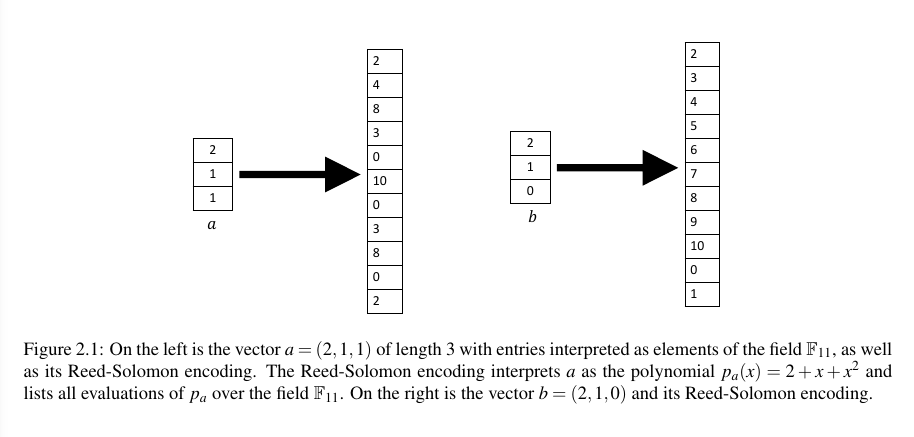
\includegraphics[scale=0.5]{vector_polynomial} 
\end{figure}


Based on similar idea, we have the following \textit{efficient probabilistic proof system}.

\begin{boxx1}[Feivalds' Algorithm] \label{def:feivalds}

Given three matrices $A$, $B$ and $C$ over $\F_p$ where $p > n^2$, verify whether $C = AB$. 

\begin{itemize}
\item Choose a random $r \in \F_p$ and let $x = (1, r, r^2, \dots, r^{n-1})$. 
\item Compute $y = Cx$ and $z = A \cdot Bx$. Compare $x$ and $y$. 
\end{itemize}

\end{boxx1}

\begin{remark}
The fastest known algorithm for computing $A \cdot B$ runs in time roughly $O(n^{2.37286})$. In contrast, the algorithm runs in time $O(n^2)$. 
\end{remark}

\subsection{Determination of Polynomials}

\textbf{Univariate polynomials}. There are two ways to \textbf{determine} a univariate polynomial of degree $n-1$  $p(X) = \sum_{i = 1}^n a_i X^{i-1}$, both of which make use vectors $a = (a_0, a_1, \dots, a_{n-1}) \in \F^n$. An apparent way is to use directly $a$ as the \textbf{coefficients} of $p(X)$. As for the alternative, recall $n$ evaluations of the polynomial $p(r_i)$ for $i = 1, \dots, n$ can completely determine the polynomial $p(X)$ as $(p -  q)(X)$ has at most $n-1$ roots considering the degree $\degg(p) \degg(q) = n-1$. Indeed, the polynomial can be established by \textbf{Univariate Lagrange Interpolation}:
\begin{equation} \label{eq:univariate-lagrange}
p(X) = \sum_{j = 0}^{n-1} a_{j+1} \cdot \delta_{j}(X)
\end{equation}
where $a_{j+1} = p(r_{j+1})$ and $\delta_j(X)$ is the polynomial of degree $n-1$

\begin{equation*}
\delta_j(X) = \frac{(X-0)(X-1) \cdots (X-j+1) (X - j - 1) \dots (X - n+1)}{(j-0)(j-1) \cdots (j-j+1) (j - j - 1) \dots (j - n+1)}
\end{equation*}
and
\[
\delta_j(r) = 
\begin{cases}
0 \text{ if } r \neq j \\
1 \text{ if } r = j
\end{cases}
\]
In summary, the $n$ evaluations $\left\{ p(0), p(1), \dots, p(n-1) \right\}$ can be thought of as an alternative specification of $p$. And they can be viewed as coefficients under the basis $\delta_i(X)$ instead of normal basis $X^i$. The method is extremely useful when an \textbf{oracle} is available for evaluating $p(X)$ while no other information is known (to the verifier). 

\textbf{Special case of cyclic multiplicative subgroup}. Normally the domain of our polynomial function is a multiplicative subgroup $H \subset \F^{\displaystyle *}$ with $\abs{H} = n$. $H$ is cyclic as well and let $H = \langle \omega \rangle$, as the $n$ powers of $\omega$ are exactly the $n$ roots of $n$-th unity in $\F$, we have
\begin{equation*}
\left( X - \omega \right) \left( X - \omega^2 \right) \cdots \left( X - \omega^{n-1} \right) \left( X - 1 \right) = X^n - 1
\end{equation*}
Computing the derivative and evaluating on $\omega^{j}$ on the two sides, we get
\begin{equation*}
\left( \omega^{j} - \omega \right) \left( \omega^{j} - \omega^2 \right) \cdots \left( \omega^{j} - \omega^{n-1} \right) \left( \omega^{j} - 1 \right) = n \omega^{jn - j} = \frac{n}{\omega^j}
\end{equation*}
Hence, in this case the Lagrange basis polynomial has a simple expression:
\begin{equation*}
\delta_j(X) = \frac{\omega^j (X^n - 1)}{ n (X - \omega^j)}
\end{equation*}

\textbf{Multivariate polynomials}. Instead of \textit{polynomial} function $p(X)$ as discussed above, consider a (general) function $f: \left\{ 0, 1 \right\}^{\nu} \rightarrow \F$. Note that to determine this function we should take all $2^v$ evaluations at all points in the domain. Next, we will show such functions have extensions in the form of \textit{multilinear polynomials} with degree $v$, thus logarithmic in the domain size $2^v$. 

\textbf{Lagrange interpolation of multilinear polynomials}.

\begin{lemma} \label{lem:MLE}
Let $f: \left\{ 0, 1 \right\}^{\nu} \rightarrow \F$ be \textbf{any} function. Then the following \textbf{multilinear polynomial (MLE) $\tilde{f}$ extends $f$}:
\begin{equation*}
\tilde{f} (x_1, \dots, x_{\nu}) = \sum_{w \in \left\{ 0, 1 \right\}^{\nu}} f(w) \cdot \chi_{w}(x_1, \dots, x_{\nu})
\end{equation*}
where, for any $w = (w_1, \dots, w_{\nu}) \in \left\{ 0, 1 \right\}^{\nu} $
\begin{equation} \label{eq:MLE-basis}
\chi_{w}(x_1, \dots, x_{\nu}) : = \prod_{i = 1}^{\nu} (x_i w_i + (1 - x_i) (1 - w_i))
\end{equation}
As $x_i = 0$ or $1$, it is easy to find $\chi_w(x_1, \dots, x_{\nu})$ is multilinear. Also if we fix $w' = (w_1', \dots, w_{\nu}') \in \left\{ 0, 1 \right\}^{\nu}$, 
\[
\chi_{w'}(x) = \begin{cases}
1 \text{ if } x = w' = (w_1', \dots, w_{\nu}') \\
0 \text{ otherwise }
\end{cases}
\]
Moreover, $\tilde{f}$ is the \textbf{unique} multilinear extension (MLE) over $\F$.
\end{lemma}

Recall that a \textbf{univariate polynomial} that extends a given function $f: \left\{ 0, 1, \dots, n-1 \right\} \rightarrow \F$ must be with degree at most $n-1$. Now suppose $n = 2^{\nu}$ and multilinear polynomials, by the above lemma, the \textbf{total degree} of the polynomial is at most $\nu$, which is logarithmic in the domain size $n = 2^{\nu}$. Multivariate polynomials with ultra-low degree in each variable turn out be especially useful when designing interactive proofs with small communication and fast verification. 

\textbf{Evaluating the multilinear extension $\tilde{f}$ of $f$}. Suppose the verifier $\mathcal{V}$ is given as input the values $f(w)$ for $w \in \left\{ 0, 1 \right\}^{\nu}$. Thus we can establish the MLE $\tilde{f}$, also we usually need to evaluate $\tilde{f}$ efficiently at any point $r \in \F^{\nu}$. 

\begin{lemma} \label{lem:evaluate-MLE}
Fix a positive integer $\nu$, and let $n = 2^{\nu}$. Given as input $f(w)$ for all $w \in \left\{ 0, 1 \right\}^{\nu}$ and a vector $r = (r_1, \dots, r_{\nu}) \in \F^{\log n}$, $\mathcal{V}$ can compute $\tilde{f}(r)$ in $O(n)$ time and $O(n)$ space. 
\end{lemma}

\begin{figure}[h]
\centering
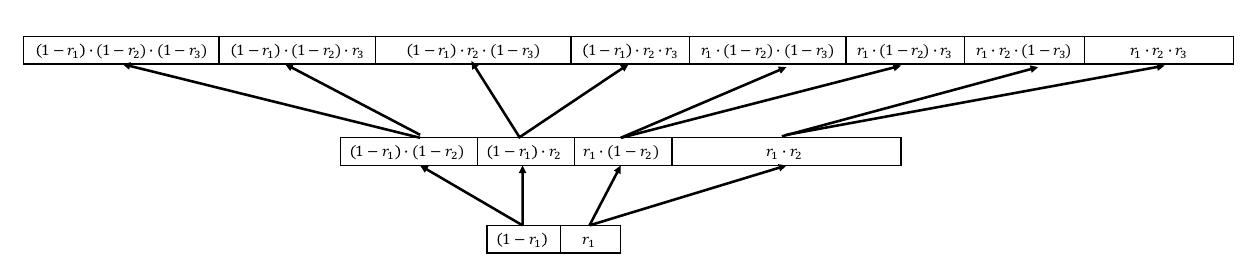
\includegraphics[scale=0.4]{eval_mle}
\end{figure}

For the fixed $r = (r_1, \dots, r_{\nu}) \in \F^{\log n}$, it suffices to establish a table where are stored $n = 2^{v}$ elements of $ \chi_{w}(r_1, \dots, r_{\nu})$ for $w \in \left\{ 0, 1 \right\}^{\nu}$ and compute the dot product with $f(w)$ which takes running time in $O(n)$. Such a table can be constructed in a recursive way as showed in the figure, thus costs $2^{\nu} = n$ memory units in total. Meanwhile, the procedure takes $\nu = \log n$ stages to construct, and the $i$-th round expands the terms $2$ times of the terms in the $i-1$-th round, thus in running time $O(2^i)$. In total, the time is $O(\sum_{j = 1}^{\log n}2^j) =O(2^{\log n}) = O(n)$.

\textbf{Distance-Amplification}. As with the case of \textit{univariate} low-degree extensions, one can think of a low-degree extension $\widetilde{f}(x)$ as a \textit{distance-amplification} of $f: \left\{ 0, 1 \right\}^v \rightarrow \mathcal{R}$. In fact, the following lemma tells that, as $\widetilde{f}$ is $v$-variate multilinear with total degree at most $v$, the probability of $\widetilde{f}$ taking random input as a root is at most $v / \abs{\F}$. Thus, the difference of two functions $f, f': \left\{ 0, 1 \right\}^v \rightarrow \mathcal{R}$ can be amplified via their extensions.

\begin{lemma}[Schwartz-Zippel] \label{lem:multivariate-root-portion}
Let $g: \F^m \rightarrow \F$ be a $m$-variate polynomial of total degree at most $d$. Then on any finite set $S \subset \F$, 
\begin{equation*}
\mathop{\Prr}_{x \leftarrow S^m} [g(x) = 0] \leq d/|S|
\end{equation*}
\end{lemma}

\subsection{Evaluation of Polynomials} \label{sec:eval-polyn}

In this section, we will study how to use inner product $\langle u, y \rangle$ for $u, y \in \F^n$ and $n$ is the number of coefficients, to represent an evaluation of $q$. Here we ask $q$ is either univariate or multilinear polynomial.

If $q$ is univariate, say, $q(X) = \sum_{i = 0}^{n-1} u_i X^i$, then for any evaluation point $z \in \F$, let $y = (1, z, z^2, \dots, z^{n-1})$ we get 
\begin{equation*}
q(z) = \langle u, y \rangle = \sum_{i = 0}^{n-1} u_i z^i
\end{equation*}

If $q$ is multilinear polynomial in $l$ variables, then via the Lagrange basis $\left\{ \chi_{w}(x_1, \dots, x_l) \right\}_{w \in \left\{ 0, 1 \right\}^l}$ we get
\begin{equation*}
q(X) = \sum_{i = 1}^{2^l} u_i \chi_i(X)
\end{equation*}
Hence, let $y = (\chi_1(z), \dots, \chi_{2^l}(z))$ we get
\begin{equation*}
q(z) = \langle u, y \rangle = \sum_{i = 1}^{2^l} u_i \chi_i(z)
\end{equation*}

\textbf{Tensor structure in the evaluation vector}. In the univariate case, suppose the polynomial degree equals to $n-1$ and $n = m^2$, thus a power of $z$ can be written as  $z^{i \cdot m + j}$ for $i, j = 1, \dots, m$. Putting the coefficient $u_{ij}$ in the similar way, then the above inner product can be expressed:

\begin{equation} \label{eq:q(z)-matrix}
\begin{pmatrix}
1 & z & \dots & z^{m-1}
\end{pmatrix}
\begin{pmatrix}
u_{11}  & u_{12}   & \dots  & u_{1m} \\
\vdots & \vdots  & \ddots & \vdots \\
u_{m1}  & u_{m2}  &\dots     & u_{mm}
\end{pmatrix}
\begin{pmatrix}
1 \\
z^{1 \cdot m} \\
\vdots \\
z^{m(m-1)}
\end{pmatrix}
= \sum_{i, j = 1}^m u_{ij} z^{im + j} = \langle u, y \rangle
\end{equation}  

See the next Figure as an example.

\begin{figure}[h]
\centering
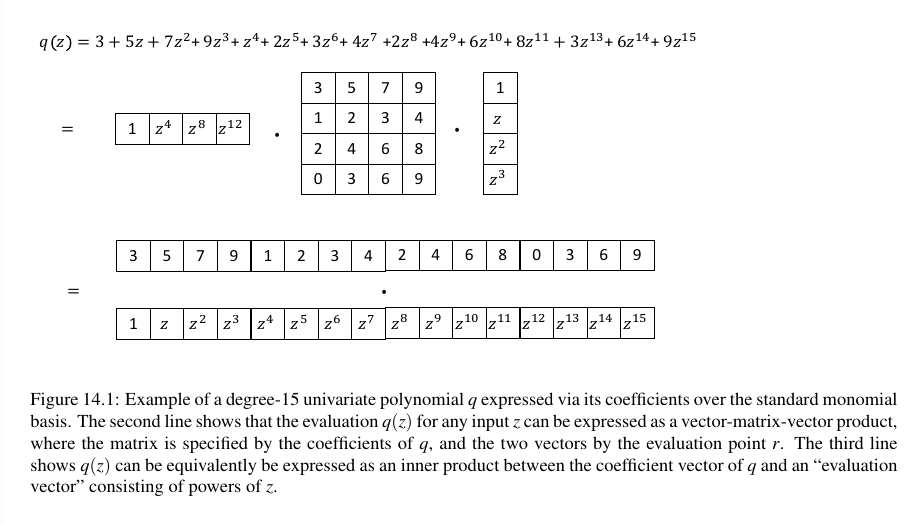
\includegraphics[scale=0.4]{eval-poly-1}
\end{figure} 

In the multilinear case $q(X_1, \dots, X_l)$, we still suppose the number of coefficients $2^l = m^2$. To "split" the vector $y = (\chi_1(z), \dots, \chi_{2^l}(z))$, recall the Language basis polynomial in the form (\ref{eq:MLE-basis}) thus we may let $z_1, z_2 \in \F^{l/2}$ denote the first half and the second half of $z \in \F^l$, then for any $w \in \left\{ 0, 1 \right\}^l$ and $z \in \F^{l}$:
\begin{equation*}
\chi_w (z) = \chi_{w_1}(z_1) \cdot \chi_{w_2}(z_2) \text{ for } w = w_1 \vert w_2, z = z_1 \vert z_2
\end{equation*}
In other words, any $l$-variate Lagrange basis polynomial can be expressed as product of two $l/2$-variate Lagrange basis polynomials. Denote the $l/2$-variate Lagrange basis polynomials as $\left\{ \chi_i' \right\}_{i = 1, \dots, m}$ for $m = 2^{l/2}$, then the inner product can be expressed as 

\begin{equation*}
\begin{pmatrix}
\chi_1'(z_1) & \chi_2'(z_1) & \dots & \chi_m'(z_1)
\end{pmatrix}
\begin{pmatrix}
u_{11}  & u_{12}   & \dots  & u_{1m} \\
\vdots & \vdots  & \ddots & \vdots \\
u_{m1}  & u_{m2}  &\dots     & u_{mm}
\end{pmatrix}
\begin{pmatrix}
\chi_1'(z_2) \\
\chi_2'(z_2) \\
\vdots \\
\chi_m'(z_2)
\end{pmatrix}
= \sum_{w \in \left\{ 0, 1 \right\}^l}  u_{w} \chi_{w}(z) = \langle u, y \rangle
\end{equation*}  

\begin{figure}[h]
\centering
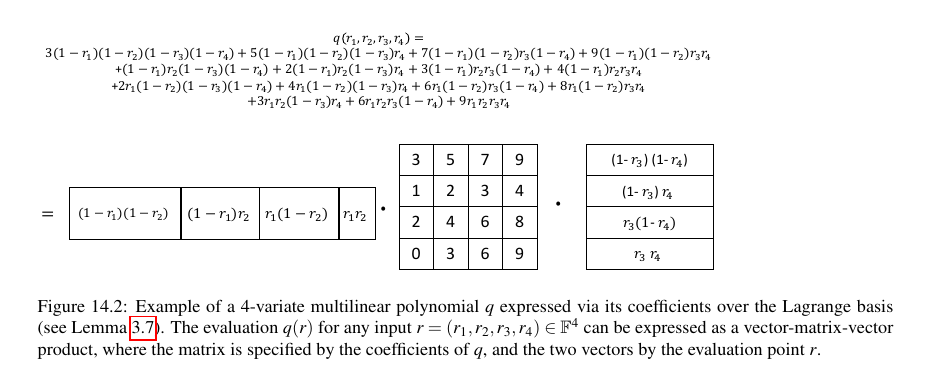
\includegraphics[scale=0.4]{eval-poly-2}
\end{figure} 

\newpage

\subsection{BLS12-381 with Pairing}

\textit{BLS12-381} is a pairing-friendly elliptic curve defined by the equation
\begin{equation*}
E /\mathbb{F}_q: \quad  y^2 = x^3 + 4
\end{equation*}

\begin{itemize}
\item the size of the base field is
\begin{equation*}
q= 0x1a0111ea397fe69a4b1ba7b6434bacd764774b84f38512bf6730d2a0f6b0f6241eabfffeb153ffffb9feffffffffaaab
\end{equation*}
for which the number of bits is $381$
\item the embedding degree $k = 12$ so that the values of pairing on BLS12-381 are within the field $\mathbb{F}_{q^k}$. 
\item the order $r$ of the (cyclic) subgroups used for pairing is
\begin{equation*}
r = 0x73eda753299d7d483339d80809a1d80553bda402fffe5bfeffffffff00000001
\end{equation*}
\item a field extension of degree $2$ regarding $\mathbb{F}_q$ is defined by 
\begin{equation*}
\mathbb{F}_{q^2} = \mathbb{F}_q[X] / (X^2 + 1) = \mathbb{F}_q[i]
\end{equation*}
\item the \textit{sextic twist} of the BLS12-381 is the elliptic curve defined over the above extension field $\mathbb{F}_{q^2}$
\begin{equation*}
E' / \mathbb{F}_{q^2}: \quad y^2 = x^3 + 4(i + 1)
\end{equation*}
this curve is isomorphic, or informally speaking, identical to BLS12-381 subject to some mapping $\phi$ between $E$ and $E'$, the mapping can be found accordingly 
\item why twist? Technically, to define the pairing we should take the second base point $Q \in E(\mathbb{F}_{q^k})$ for $k = 12$ and consider the cyclic group $\langle G \rangle \subset E(\mathbb{F}_{q^k})$. But the field $\mathbb{F}_{q^k}$ is large where the computation is expensive, then we transform such computations to another isomorphic (almost identical) curve with smaller base field $\mathbb{F}_{p^2}$. Eg:
\begin{equation*}
E'(\mathbb{F}_{q^2}) \ni G_1 + G_2 \mapsto \phi(G_1) + \phi(G_2) \in E(\mathbb{F}_{q^k})
\end{equation*}
\end{itemize}

\textbf{Pairing over BLS12-381}. With the above notations, we can fix two base points $P \in E(\mathbb{F}_q)$ and $Q \in E'(\mathbb{F}_{p^2})$, then for the two cyclic groups of order $r$: $G_1 = \langle P \rangle \subset E(\mathbb{F}_q)$ and $G_2 = \langle Q \rangle \subset E'(\mathbb{F}_{q^2})$ and the group of $r$-th roots $G_T \subset \mathbb{\F}_{q^k}$, define the pairing
\begin{equation*}
\begin{split}
e: \quad G_1 \times G_2 & \rightarrow G_{T} \subset \mathbb{F}_{q^k} \\
(P_1, Q_1) & \mapsto e(P_1, Q_1) = (\frac{f_P(Q_1 + R)}{f_P(R)})^{(q^k - 1) / r}
\end{split}
\end{equation*}
where $f_P$ can be computed efficiently by \textit{Miller's algorithm}, an iteration over the binary representation $r = (b_{n-1}, b_{n-2}, \dots, b_0)$ is called a \textit{Miller loop}. 

\begin{equation*}
\begin{split}
e(A, B) &= e(\alpha_1, \beta_1) \cdot e(\alpha_2, \beta_2) \cdot e(\alpha_3, \beta_3) \quad \text{ for } (\alpha_1, \beta_1) \text{ is the verification key} \\
e(-\alpha_1, \beta_1) &= e(-A, B) \cdot  e(\alpha_2, \beta_2) \cdot e(\alpha_3, \beta_3) \\
& = \left( e'(-A, B) \cdot  e'(\alpha_2, \beta_2) \cdot e'(\alpha_3, \beta_3) \right)^{(q^k - 1) / r}
\end{split}
\end{equation*}



\section{Interactive Proofs}


\subsection{The Sum-Check Protocol}

\begin{boxx1}[Sum-Check Protocol] \label{def:sum-check-protocol}
Let $g \in \F[x_1, \dots, x_{\nu}]$ be a $\nu$-variate polynomial defined over a finite field $\F$. The prover is required to provide the verifier with the following sum:
\begin{equation} \label{eq:sum-check-protocol}
H : = \sum_{b_1 \in \{0, 1\}} \:  \sum_{b_2 \in \{0, 1 \}} \dots  \sum_{b_v \in \{0, 1 \}} \: g(b_1, \dots, b_{\nu})
\end{equation}
In other words, the sum is computed by values of $g$ in traversal of the $2^{v}$ binary strings $s = b_1 \dots b_{v}$.

\begin{itemize}
\item At the start of the protocol, the prover $\mathcal{P}$ sends a value $C_1$ \textbf{claimed} to equal the value $H$ defined in (\ref{eq:sum-check-protocol}). 
\item In the $1$st round 
\begin{enumerate}
\item\label{item:3} the prover $\mathcal{P}$ sends the univariate polynomial $g_1(X_1)$ \textbf{claimed} to equal
\begin{equation*}
s_1(X_1) = \sum_{(x_2, \dots, x_{\nu}) \in \left\{ 0, 1 \right\}^{\nu - 1}}  g(X_1, x_2, \dots, x_{\nu})
\end{equation*}
\item\label{item:4} The verifier $\mathcal{V}$ checks if $\degg(g_1) \leq \degg_1(g)$ and 
\begin{equation*}
C_1 = g_1(0) + g_1(1)
\end{equation*}
Here $\degg_j(g)$ denotes the degree of $g(X_1, \dots, X_{\nu})$ in variable $X_j$.
\item\label{item:5} If no rejection, $\mathcal{V}$ chooses a random element $r_1 \in \F$ and sends $r_1$ to $\mathcal{P}$. 
\end{enumerate}
\item In the $j$-th round for $1 < j < \nu$, 
\begin{enumerate}
\item\label{item:6} $\mathcal{P}$ sends to $\mathcal{V}$ a univariate polynomial $g_j(X_j)$ \textbf{claimed} to equal 
\begin{equation*}
s_j(X_j) = \sum_{x_{j+1}, \dots, x_{\nu} \in \left\{ 0, 1 \right\}^{\nu - j}}  g(r_1, \dots, r_{j-1}, X_j, x_{j+1}, \dots, x_{\nu})
\end{equation*}
\item\label{item:7} $\mathcal{V}$ checks that $\degg(g_j) \leq \degg_j(g)$ and 
\begin{equation} \label{eq:key-step-sum-check}
g_{j-1}(r_{j-1}) = g_j(0) + g_j(1)
\end{equation}
\item\label{item:8} If no rejection, $\mathcal{V}$ chooses a random element $r_j \in \F$ and sends to $\mathcal{P}$.
\end{enumerate}
\item In the final round 
\begin{enumerate}
\item\label{item:9} $\mathcal{P}$ sends to $\mathcal{V}$ a univariate polynomial $g_{\nu}(X_{\nu})$ \textbf{claimed} to equal
\begin{equation*}
g(r_1, \dots, r_{\nu - 1}, X_{\nu})
\end{equation*}
\item\label{item:14} $\mathcal{V}$ checks that $\degg(g_{\nu}) \leq \degg_{\nu}(g)$ and check 
\begin{equation*}
g_{\nu - 1} (r_{\nu -1}) = g_{\nu} (0) + g_{\nu} (1)
\end{equation*}
\item\label{item:10} If no rejection, $\mathcal{V}$ chooses a random $r_{\nu} \in \F$ and check the value of $g_{\nu}(r_{\nu})$ with  $g(r_1, \dots, r_{\nu})$ by a single oracle query to $g$, rejecting or not. 
 
\end{enumerate}
\item  If $\mathcal{V}$ has not yet rejected, $\mathcal{V}$ halts and accepts.
\end{itemize}

\end{boxx1}

\begin{enumerate}[(a)]
\item\label{item:1} In order to check the validity of $C_1$, we may compute the sum over the last $v-1$ variables $X_2, \dots, X_v$ first which leads to a univariate polynomial

\begin{equation*}
g_1(X_1) = \sum_{(x_2, \dots, x_{\nu}) \in \left\{ 0, 1 \right\}^{\nu - 1}}  g(X_1, x_2, \dots, x_{\nu})
\end{equation*}
and finally sum $g_1(X_1)$ over $X_1 \in \left\{0, 1  \right\}$. Suppose $g_1(X_1)$ is correctly computed, it suffices to verify $g_1(0) + g_1(1) = C_1$.
\item\label{item:2} To verify the assumption of correctness of $g_1(X_1)$, at the end of the $1$st round, $\mathcal{V}$ sends a random $r_1 \leftarrow \F$ to $\mathcal{P}$ which will be used to compare $g_1(r_1) = s_1(r_1)$ in the $2$nd round. Note the usage of $r_1$ renders the determination of $g_1(X)$ more efficient. $s_1(r_1)$ is defined as the sum over $2^{\nu - 1}$ evaluations of the $\nu -1$-variate polynomial $g(r_1, X_2, \dots, X_n)$. Hence, by a \textbf{recursive} way $\mathcal{P}$ and $\mathcal{V}$ should apply this protocol on the claimed value $g_1(r_1)$ and the sum over the $v-1$-variate polynomial $g(r_1, X_2, \dots, X_v)$. More precisely
\begin{equation*}
g_1(r_1) = \sum_{(x_2, \dots, x_{\nu}) \in \left\{ 0, 1 \right\}^{\nu - 1}}  g(r_1, x_2, \dots, x_{\nu})
\end{equation*}
The recursion goes forward until the $v$-th round where $\mathcal{P}$ sends the polynomial
\begin{equation*}
g_v(X_v) = g(r_1, \dots, r_{v-1}, X_v)
\end{equation*}
\item\label{item:12} In the $\nu$-th round, it suffices to use a single query of $g$ on one input value $(r_1, \dots, r_{\nu})$ to get $s_v(r_1, \dots, r_v)$, and compare the claimed value $g_v(r_1, \dots, r_v) = s_v(r_1, \dots, r_v)$. Also, the recursion terminates at this point. 
\item\label{item:78} The key technique is: in the $j$-th round the prover introduces the polynomial $g_j(X_j)$, then using random evaluation the verifier checks the correctness of the polynomial $g_{j-1}(X_{j-1})$ sent by the prover in the $j-1$-th round, i.e the equation (\ref{eq:key-step-sum-check}).
\item\label{item:16} It is important to notice that during the whole protocol, the verifier $\mathcal{V}$ only checks values using \textbf{the polynomials given by $\mathcal{P}$}, except for the last round when $\mathcal{V}$ should evaluate $g$ at the point $r = (r_1, \dots, r_{\nu})$. 
\end{enumerate}

\textbf{Completeness and Soundness}. 

\begin{boxx2}
For any specified $H \in \F$, let $\mathcal{L}$ be the language of polynomials $g$ (given as an oracle) such that

\begin{equation*}
H = \sum_{b_1 \in \{0, 1\}} \:  \sum_{b_2 \in \{0, 1 \}} \dots  \sum_{b_v \in \{0, 1 \}} \: g(b_1, \dots, b_{\nu})
\end{equation*}
The sum-check protocol is an interactive proof system for $\mathcal{L}$ with completeness error $\delta_c = 0$ and soundness error $\delta_s \leq \nu d / |\F|$.
\end{boxx2}

\begin{proof}
Completeness is evident. For the soundness, suppose the claimed $C_1 \neq H$ which is the true value, let $i$ be \textit{the least} index such that $X_{i}, X_{i+1}, \dots, X_v$ are evaluated correctly on $g$ (remember we count the variable in the reverse order). Then in the $i$-th round Equation (\ref{eq:key-step-sum-check}) will no more hold \textit{with high probability}:
\begin{equation*}
g_{i-1}(r_{i-1}) \neq g_{i}(0) + g_{i}(1)
\end{equation*}
In other words, the equality still holds with a probability at most $d/|\F|$. Since it may happen for any round $i = 1, \dots, \nu$, the result follows the union bound. 
\end{proof}

\textbf{Discussion of costs}. 
\begin{center}
% \color{Red}
\begin{tabular} { | m{5cm} | m{1cm} | m{4cm} | m{5cm} | }
\hline
Communication        & rounds   & $\mathcal{V}$ time  & $\mathcal{P}$ time \\
\hline
$O(\sum_{i = 1}^{\nu} \degg_i(g))$ field elements  & $\nu$  & $ O(\nu + \sum_{i = 1}^{\nu} \degg_i(g)) + T$ & $ O(\sum_{i=1}^{\nu} \degg_i(g) \cdot 2^{\nu - i} \cdot T) = O(2^{\nu} \cdot T)$ if $\degg_i(g) = O(1)$ for all $i$ \\
\hline
\end{tabular}
\end{center}

\begin{enumerate}[(a)]
\item\label{item:11} Recall the specification of degree $d$ polynomial needs $d + 1$ (field) elements. Thus, the \textbf{prover-to-verifier communication} is 
\begin{equation*}
\sum_{i = 1}^{\nu} (\degg_i(g) + 1) = \nu + \sum_{i = 1}^{\nu} \degg_i(g)
\end{equation*}
Including the random elements $r_i$ in \textbf{verifier-to-prover communication} of each round, and suppose the degree for each variable is bounded $\degg_i(g) = O(1)$, then the total communication cost is $O(\nu)$. 
\item\label{item:13} Considering the running time of $\mathcal{V}$ is almost constant in each round: verifying an equality and sending back a random element, the running time of verifier is proportional to the total communication, \textbf{plus} the cost of a single oracle query to $g$ to compute $g(r_1, \dots, r_{\nu})$ which we denote by $T$. 
\item\label{item:15} Regarding the running time of the prover $\mathcal{P}$, in the $j$-th round $\mathcal{P}$ can specify $g_j$ by sending for each $i \in \left\{ 0, 1, \dots, \degg_j(g) \right\}$ the value:
\begin{equation*}
g_j(i) = \sum_{(x_{j+1}, \dots, x_r) \in \left\{ 0, 1 \right\}^{\nu - j}} g(r_1, \dots, r_{j-1}, i, x_{j + 1}, \dots, x_{\nu})
\end{equation*}
Thus it takes $(1 + \degg_j(g)) \cdot 2^{\nu - j}$ evaluations of $g$. Suppose all degrees $\degg_i(g)$ is bounded, the total running time of $\mathcal{P}$ is thus $O(2^{\nu} \cdot T)$.
\end{enumerate}

\textbf{Application of the Sum-Check Protocol - Matrix Multiplication (M{\footnotesize AT}M{\footnotesize ULT})}

Given $n \times n$ input matrix $A, B$, in order to verify the product matrix $A \cdot B$ equals $C$, we have the random algorithm of Feivalds' algorithm \ref{def:feivalds}. We now interpret $A, B$ and $C$ as functions $f_A, f_B, f_C$ as mappings
\begin{equation*}
\begin{split}
& f_A: \left\{ 0, 1 \right\}^{\log n} \times \left\{ 0, 1 \right\}^{\log n} \rightarrow \F \\
 & (i_1, \dots, i_{\log n}, j_1, \dots, j_{\log n}) \mapsto A_{ij}
\end{split}
\end{equation*}
As usual, $\widetilde{f}_A, \widetilde{f}_B$ and $\widetilde{f}_C$ denote the MLE of $f_A, f_B, f_C$, mappings from $\F^{\log n} \times \F^{\log n} \rightarrow \F$. 

\begin{lemma}
\begin{equation*}
\widetilde{f}_C(x, y) = \sum_{b \in \left\{ 0, 1 \right\}^{ \log n}} \widetilde{f}_A(x, b) \cdot \widetilde{f}_B(b, y)
\end{equation*}
\end{lemma}

It suffices to notice the right-hand side is multilinear in $x, y$ and coincident with the left-hand side at all $(x, y) \in \left\{ 0, 1 \right\}^{\log n} \times \left\{ 0, 1 \right\}^{\log n}$.

\begin{remark} \label{sec:matrix-mult}
Fix $x_{0}, y_{0}$, let $g(z) = \widetilde{f}_A(x_{0}, z) \cdot \widetilde{f}_B(z, y_{0})$. Thus we can apply the sum-check protocol to the Matrix Multiplication (M{\footnotesize AT}M{\footnotesize ULT}) problem. And in the round $k$, the polynomial claimed by $\mathcal{P}$ is

\begin{equation*}
\sum_{b_{k+1} \in \left\{ 0, 1 \right\}} \dots \sum_{b_{\log n} \in \left\{ 0, 1 \right\}} g(r_1, \dots, r_{k-1}, X, b_{k+1}, \dots, b_{\log n})
\end{equation*}

and to specify this polynomial, since it is of degree $2$ the prover $\mathcal{P}$ can just send the values at $X = 0, 1, 2$. Hence, $\mathcal{P}$ should evaluate $g(z) = \widetilde{f}_A(x_{0}, z) \cdot \widetilde{f}_B(z, y_{0})$ at points
\begin{equation*}
z \in \left( r_1, \dots, r_{k-1}, \left\{ 0, 1, 2 \right\}, b_{k+1}, \dots, b_{\log n} \right): b_j \in \left\{ 0, 1 \right\}
\end{equation*}
Therefore, there are $3 \cdot n/2^k$ such points in round $k$, and for each point the evaluation in $z$ of $\widetilde{f}_A(x_{0}, z)$ runs in $O(n^2)$ as $(x_0, z)$ are inputs of a matrix, according to the Lemma \ref{lem:evaluate-MLE}. Rather than considering directly the running time of $\mathcal{P}$ in $n^2 \cdot 3 \cdot n/2^k = O(n^{3})$, let's have a closer look at the evaluation $\widetilde{f}_A$ at $(x_0, z_0) \in \left\{ 0, 1 \right\}^{\log n} \times  \left\{ 0, 1 \right\}^{\log n}$:
\begin{equation*}
 \widetilde{f}_A(x_{0}, z_{0}) = \sum_{i, j \in \left\{ 0, 1 \right\}^{\log n}} A_{ij} \cdot \chi_{ij}(x_{0}, z_{0})
\end{equation*}
And $\chi_{ij}(x_{0}, z_{0}) = 0$ when any \textbf{binary part} in $(x, z)$ is not equal to the corresponding binary part in $(i, j)$, based on the Lemma \ref{lem:MLE}. Hence, for one evaluation at $(b_{k+1}, \dots, b_{\log n})$ where $b_j \in \left\{ 0, 1 \right\}$, only some terms $\chi_{ij}(x_{0}, z_{0})$ of $ \widetilde{f}_A(x_{0}, z_{0})$ count whose trailing coordinates are the same as $(b_{k+1}, \dots, b_{\log n})$. In this way, all points $(b_{k+1}, \dots, b_{\log n})$ make \textbf{only one evaluation} of $\widetilde{f}_A(x_{0}, z_{0})$ which costs $O(n^{2})$, rather than $n/2^k$ times. 

\end{remark}



\subsection{The GKR Protocol}

The GKR protocol describes a remarkable \textbf{interactive} proof protocol in terms of the \textbf{arithmetic circuit evaluation problem}. In this problem, $\mathcal{P}$ and $\mathcal{V}$ first agree on a \textbf{log-space uniform} arithmetic circuit $\mathcal{C}$ of fan-in $2$ over a finite field $\F$, and the goal is to compute the value of the output gates of the circuit $\mathcal{C}$. A log-space uniform circuit $\mathcal{C}$ is one that possesses a succinct implicit description, in the sense that a so-called \textbf{logarithmic-space} algorithm takes as input the label of a gate $a$, then outputs the labels of all of $a$'s neighbors also determines if $a$ is an addition gate or a multiplication gate. 

\textbf{Notations and Functions}. 

Suppose we are given a \textbf{layered arithmetic circuit} $\mathcal{C}$ of fan-in two, size (i.e., number of gates) $S$, depth $d$ and number of variables $n$. Number the layers from $0$ to $d$, with $0$ being the output layer and $d$ being the input layer. Let $S_i$ denote the number of gates at layer $i$ of the circuit $C$ which equals $2^{k_i}$ by assumption. 

\begin{itemize}
\item Number the $2^{k_i}$ gates at layer $i$ from $0$ to $S_i - 1$ and convert into binary labels in $\left\{ 0, 1 \right\}^{k_i}$, let 
\begin{equation*}
W_i: \left\{ 0, 1 \right\}^{k_i} \rightarrow \F
\end{equation*}
denote the function that takes the input a gate at layer $i$, and outputs the corresponding value.
As usual, let $\widetilde{W_i}$ denote the multilinear extension of $W_i$. See the picture below:
\begin{figure}[h]
\centering
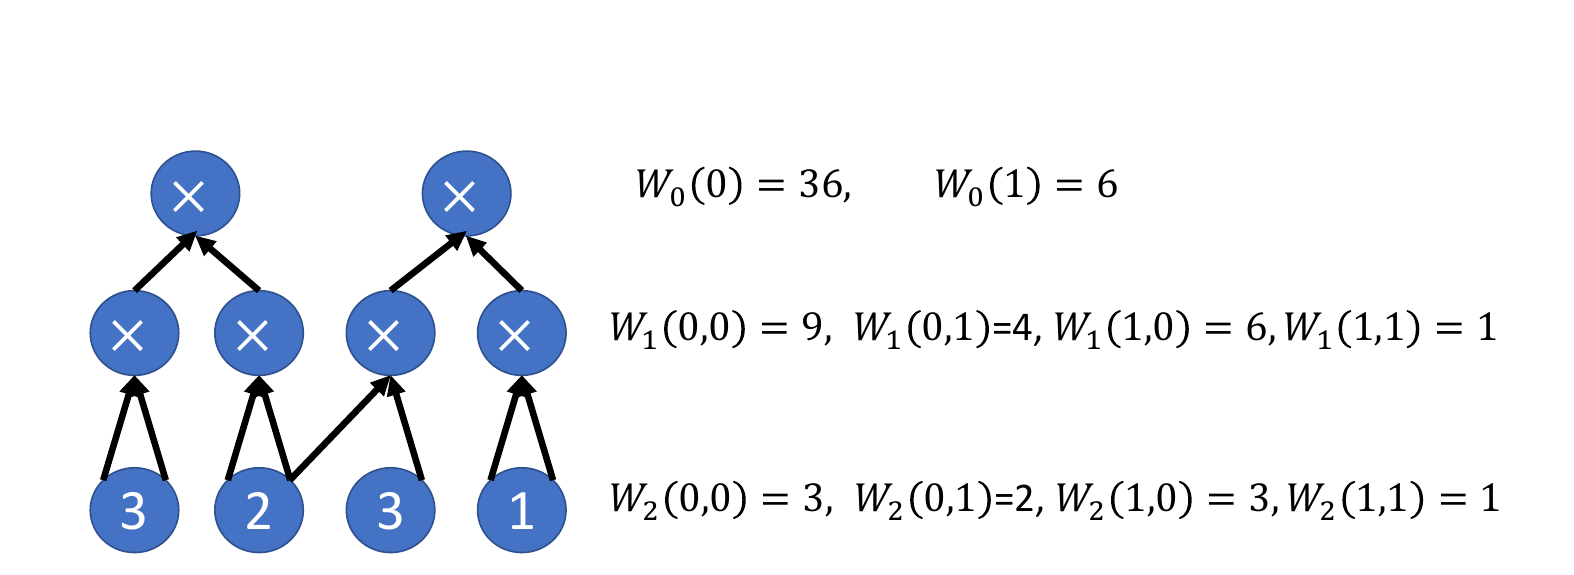
\includegraphics[scale=0.3]{GKR_01}
\end{figure} 
\item Let 
\begin{equation*}
\text{in}_{1, i}, \text{in}_{2, i}: \left\{ 0, 1 \right\}^{k_i} \rightarrow \left\{ 0, 1 \right\}^{k_{i+1}}
\end{equation*}
denote the functions that takes as input the label $a$ of a gate at layer $i$, and respectively output the label of the first and second in-neighbor of gate $a$, which are summed or multiplied up into the gate $a$. 
\item Define two functions that take the input $(a,b,c)$, one gate at layer $i$ and two gates at layer $i+1$ 
\begin{equation*}
\text{add}_i, \text{mult}_i: \left\{ 0, 1 \right\}^{k_i + 2k_{i+1}} \rightarrow \left\{ 0, 1 \right\}
\end{equation*}
the return value is $1$ iff $(b, c) = (\text{in}_{1, i}(a) = b, \text{in}_{2, i}(a) = c)$ and gate $a$ is an addition (respectively, multiplication) gate. As usual, their MLE are denoted by $\widetilde{\text{add}_i}, \widetilde{\text{mult}_i}$. For example, consider the circuit depicted in the figure below: as there are $2 = 2^1$ gates in layer $0$ and $4 = 2^2$ gates in layer $1$, for $\text{mult}_0$ defined over domain $\left\{ 0, 1 \right\} \times \left\{ 0, 1 \right\}^2 \times \left\{ 0, 1 \right\}^2$. And the return value is $1$ for the two inputs $(0, (0, 0), (0, 1))$ (the most left ones) and $(1, (1, 0), (1, 1))$. Similarly, $\text{mult}_1$ maps the domain $\left\{ 0, 1 \right\}^2 \times \left\{ 0, 1 \right\}^2 \times \left\{ 0, 1 \right\}^2$, and returns $1$ for the inputs: $((0, 0), (0, 0), (0, 0)), ((0, 1), (0, 1), (0, 1))$ etc. 

\end{itemize}

\begin{figure}[h] \label{fig:circuit-MLE}
\centering
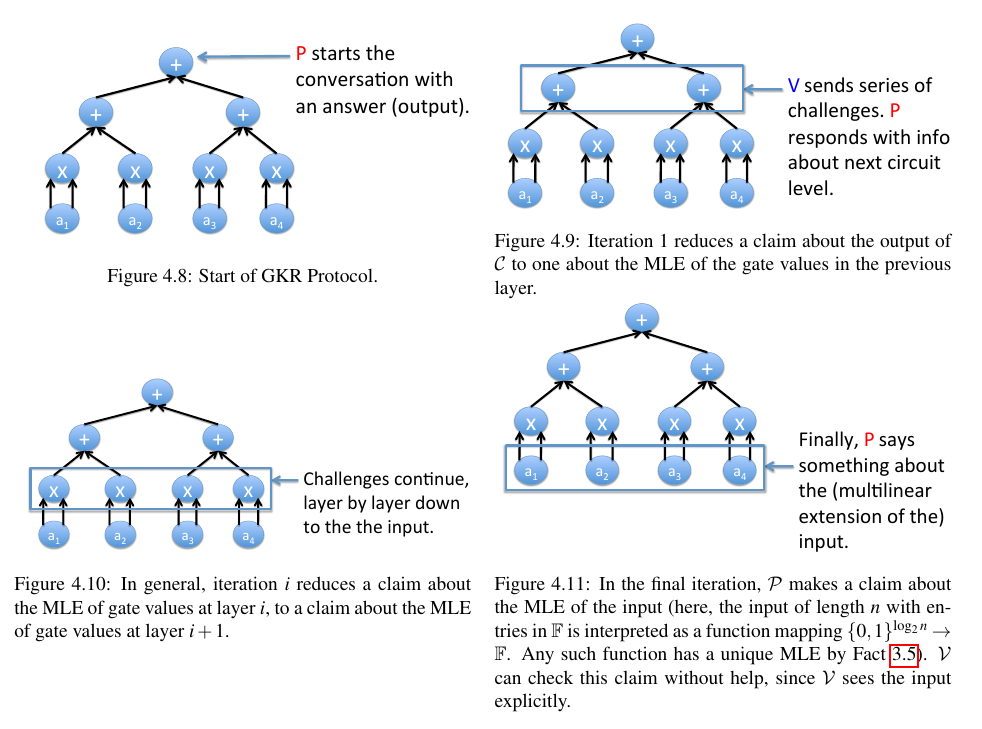
\includegraphics[scale=0.5]{GKR_02}
\end{figure}

\textbf{Heuristics of the protocol}. 
\begin{itemize}
\item The prover $\mathcal{P}$ claims to know the values of all output gates in layer $0$, i.e. in the form of function
\begin{equation*}
D: \left\{ 0, 1 \right\}^{k_0} \rightarrow \F
\end{equation*}
\textbf{Equivalently}, $\mathcal{P}$ gets to know its \textbf{MLE} $\tilde{D}$. Thus, as usual this polynomial can be (approximately) determined by the evaluation at a random $r_0 \leftarrow \F^{k_0}$:
\begin{equation*}
\widetilde{D}(r_0) = \widetilde{W_0}(r_0)
\end{equation*}
\item The verifier $\mathcal{V}$ is supposed to know no more than the input values in layer $d$, thus is not able to evaluate $\widetilde{W_0}(r_0)$ directly. The strategy is to \textbf{reduce} the claim about $\widetilde{W_i}(r_{i})$ to a claim about $\widetilde{W}_{i+1}(r_{i+1})$ for some $r_{i+1} \in \F^{k_{i+1}}$, in the sense that it is safe for $\mathcal{V}$ to assume $\widetilde{W_i}(r_{i})$ is true as long as  $\widetilde{W}_{i+1}(r_{i+1})$ is true. As analogy in the sum-check protocol, the $i$-th round is based on correctness of $\widetilde{W}_{i+1}(z)$, which can be determined via evaluation at a random point $r_{i+1}$ in the $(i+1)$-th round. This reduction is accomplished by applying the \textbf{sum-check protocol}. By the final round, $\mathcal{V}$ has direct access to the gate which are just input values, as showed in the second figure. 
\item The key connection between $\widetilde{W_i}(r_{i})$ and $\widetilde{W}_{i+1}(r_{i+1})$ is the following
\begin{lemma}
Recall $W_i: \left\{ 0, 1 \right\}^{k_i} \rightarrow \F$ maps the gate labels in layer $i$ to $\F$, thus for its MLE $\widetilde{W}_i$ and any $z \in \F^{k_i}$ we have
\begin{equation*}
\widetilde{W}_i(z) = \sum_{b, c \in \left\{ 0, 1 \right\}^{k_{i+1}}} \widetilde{\text{add}_i}(z, b, c)(\widetilde{W}_{i+1}(b) + \widetilde{W}_{i+1}(c)) + \widetilde{\text{mult}}_i(z, b, c)(\widetilde{W}_{i+1}(b) \cdot \widetilde{W}_{i + 1}(c))
\end{equation*}
\end{lemma}
It suffices to notice that the right-hand side is a \textbf{multilinear function in $z \in \F^{k_i} $} and the two sides coincident at values $z \in \left\{ 0, 1 \right\}^{k_i}$, then the result follows by the Lemma \ref{lem:MLE}. 
\item Let $z = r_i \in \F^{k_i}$ as in the above equation, the sum-check protocol can be applied to $\widetilde{W}_i(r_i)$ for the \textbf{polynomial in $b, c$} (thus, $b, c \in \F^{k_{i+1}}$):
\begin{equation*}
f_{r_i}^{(i)}(b, c) =  \widetilde{\text{add}_i}(r_i, b, c)(\widetilde{W}_{i+1}(b) + \widetilde{W}_{i+1}(c)) + \widetilde{\text{mult}}_i(r_{i}, b, c)(\widetilde{W}_{i+1}(b) \cdot \widetilde{W}_{i + 1}(c))
\end{equation*}
Recall in the sum-check protocol, $\mathcal{V}$ need not to know the specification of $f_{r_i}^{(i)}$ so long as $\mathcal{V}$ can evaluate $f_{r_i}^{(i)}$ at a random point $(b^{*}, c^{*}) \in \F^{k_{i+1}} \times \F^{k_{i+1}}$. For now, assume $\mathcal{V}$ can perform the evaluations on $\widetilde{\text{add}_i}(r_i, b^{*}, c^{*})$ and $\widetilde{\text{mult}}_i(r_{i}, b^{*}, c^{*})$ without $\mathcal{P}$ in $O(k_i + k_{i+1})$, it remains for $\mathcal{V}$ to evaluate on $\widetilde{W}_{i+1}(b^{*}), \widetilde{W}_{i+1}(c^{*})$. 
\item Note the fact that $\widetilde{W}_{i+1}(b^{*})$ and $\widetilde{W}_{i+1}(c^{*})$ can be left to the $i+1$ round, which establishes connection from $i$ to $i+1$ round. Meanwhile, we must establish a reduction from verifying two values $\widetilde{W}_{i+1}(b^{*})$ and $\widetilde{W}_{i+1}(c^{*})$ to one $\widetilde{W}_{i+1}(r_{i+1})$, in the sense that  it is safe for $\mathcal{V}$ to accept the claimed values of $\widetilde{W}_{i+1}(b^{*})$ and  $\widetilde{W}_{i+1}(c^{*})$ as long as the value of $\widetilde{W}_{i+1}(r_{i+1})$ is as claimed for a random $r_{i+1}$.  This can be solved by restricting $\widetilde{W}_{i+1}$ over the line passing the two points $b^{*}$ and $c^{*}$ in the domain $\F^{k_{i+1}}$. Note that the (straight) line can be replaced by any curve when three or more points are required. 
\begin{lemma} \label{lem:line-point}
Composite the parameterized line $l: \F \rightarrow \F^{k_{i+1}}$ where $l(0) = b^{*}$ and $l(1) = c^{*}$, with $\widetilde{W}_{i+1}$:
\begin{equation*}
q = \widetilde{W}_{i+1} \circ l: \F \rightarrow  \F^{k_{i+1}} \rightarrow \F
\end{equation*}
thus $q(0) = \widetilde{W}_{i+1}(b^{*})$ and $q(1) = \widetilde{W}_{i+1}(c^{*})$. Suppose for another function $q'$ such that $q' \neq \widetilde{W}_{i+1} \circ l$, then at least with probability $1 - k_{i+1}/|\F|$ for $r \leftarrow \F$, we have $q'(r) = \widetilde{W}_{i+1}(l(r))$. This gives a way that evaluations of a given function at several points, can be approximately determined by correctness of one evaluation at a random point only.
\end{lemma} 
\item By the above discussion, in order to finish the sum-check protocol in the $i$-th round, the verifier $\mathcal{V}$ can ask $\mathcal{P}$ to provide with $\widetilde{W}_{i+1}(b^{*})$ and $\widetilde{W}_{i+1}(b^{*})$ for the last step's evaluation of $f_{r_i}^{(i)}$. The two claimed values can be verified by the polynomial $\widetilde{W}_{i+1}(z)$ given by $\mathcal{P}$ and its evaluation $\widetilde{W}_{i+1}(r_{i+1})$ in the next round.  
\end{itemize}

\begin{boxx1}[the GKR Protocol] \label{def:GKR-protocol}
Given a layered arithmetic circuit $\mathcal{C}$ of depth $d$ and fan-in two on input $x \in \F^n$. The prover $\mathcal{P}$ is required to provide the verifier $\mathcal{V}$ with the values of outputs of $\mathcal{C}$. Throughout, $k_i$ denotes $\log_2(S_i)$ where $S_{i}$ is the number of gates at layer $i$ of $\mathcal{C}$. 
\begin{itemize}
\item At the start of the protocol, $\mathcal{P}$ sends a function $D: \left\{ 0, 1 \right\}^{k_0} \rightarrow \F$ claimed to equal $W_0$. 
\item $\mathcal{V}$ picks a random $r_0 \in \F^{k_0}$ and gets $m_0 = \widetilde{D}(r_0)$. The remainder of the protocol is devoted to confirming that $m_0 = \widetilde{W}_0(r_0)$.
\item For $i = 0, 1, \dots, d-1$ where $d$ is the layer of inputs
\begin{enumerate}[$\circ$]
\item\label{item:17} Define the $(2k_{i+1})$-variate polynomial in $b, c$
\begin{equation*}
f_{r_i}^{(i)}(b, c) =  \widetilde{\text{add}_i}(r_i, b, c)(\widetilde{W}_{i+1}(b) + \widetilde{W}_{i+1}(c)) + \widetilde{\text{mult}}_i(r_{i}, b, c)(\widetilde{W}_{i+1}(b) \cdot \widetilde{W}_{i + 1}(c))
\end{equation*}
$\mathcal{P}$ claims that $m_i = \sum_{b, c \in \left\{ 0, 1 \right\}^{k_{i+1}}} f_{r_i}^{(i)}(b, c)$. Consequently, $\mathcal{P}$ and $\mathcal{V}$ apply the sum-check protocol to $f_{r_i}^{(i)}$
\begin{enumerate}[-]
\item\label{item:51} By assumption of being \textbf{log-space uniform}, the functions $ \widetilde{\text{add}_i}(r_i, b, c)$ and $\widetilde{\text{mult}}_i(r_{i}, b, c)$ can be easily computed by the verifier. 
\item\label{item:22} Regarding $\mathcal{V}$'s final check for the random point $(b^{*}, c^{*}) \in \F^{k_{i+1}} \times \F^{k_{i+1}}$, $\mathcal{P}$ claims to $\mathcal{V}$ the function $q_{i+1} = \widetilde{W}_{i+1} \circ l$ where $l(0) = b^{*}$ and $l(1) = c^{*}$
\item\label{item:23} $\mathcal{V}$ simply finishes the sum-check protocol after the final evaluation using $q_{i+1}(0) = \widetilde{W}_{i+1}(b^{*})$ and $q_{i+1}(1) = \widetilde{W}_{i+1}(c^{*})$. 
\end{enumerate}
\item\label{item:24} $\mathcal{V}$ chooses $r^{*} \in \F$ at random and sets $r_{i+1} = l(r^{*})$, compute $m_{i+1} = \widetilde{W}_{i+1}(r_{i+1})$ which is reserved for next round's use.
\end{enumerate}
\item $\mathcal{V}$ checks directly $m_d = \widetilde{W}_d(r_d)$ using the Lemma \ref{lem:evaluate-MLE}. Note $\widetilde{W}_d$ is the MLE of the input to the protocol. 
\end{itemize}
\end{boxx1}

\textbf{Costs of the protocol}. 

\begin{itemize}
\item \textbf{The communication cost}
\begin{enumerate}[$\circ$]
\item\label{item:18} The polynomial involved in the sum-check protocol $f_{r_i}^{(i)}$ is a $(2k_{i+1})$-variate polynomial of degree at most $2$ in each variable. Thus the sum-check protocol requires $2k_{i+1}$ rounds with $3$ field elements transmitted per round. 
\item\label{item:19} Summing up all iterations $ i = 0, \dots, d - 1$, the communication cost is in $O(S_0 + d \log S)$ given $S_0$ is the number of outputs at layer $0$ and $k_{i+1} \leq \log S$.
\end{enumerate}

\item \textbf{$\mathcal{V}$'s runtime} The time cost to $\mathcal{V}$ is $O(n + d \log S + t + S_0)$.
\begin{enumerate} [$\circ$]
\item\label{item:20} $S_0$ term is the time required to read the claimed output and to evaluate its MLE $\widetilde{D}(r_0)$. 
\item\label{item:21} Recall in each sum-check protocol, $\mathcal{V}$ runs in $O(k_{i+1})$ since the degree is bounded by $2$ and the final evaluation is trivial. Hence, the $d \log S$ term is the time for $\mathcal{V}$ to send messages to $\mathcal{P}$ and check the messages from $\mathcal{P}$. 
\item\label{item:25} $t$ is the amount of time for $\mathcal{V}$ to evaluate $ \widetilde{\text{add}_i}$ and $\widetilde{\text{mult}}_i$ at random input for each layer $i$. 
\item\label{item:26} $n$ is due to the time to evaluate $\widetilde{W}_d(r_d)$. 
\item\label{item:27} Assume $t$ is low order and $S_0 = 1$, then $\mathcal{V}$ runs in time $O(n + d \log S)$.
\end{enumerate}

\item \textbf{$\mathcal{P}$'s runtime} The time cost is $\text{polylog}(S)$.

\begin{enumerate} [$\circ$]
\item\label{item:28} In the $t$-th round of the sum-check protocol for layer $i$, $\mathcal{P}$ needs specify $f_{r_i}^{(i)}$ by its evaluations at $X_{t} = 0, 1, 2$ for $t \in \left\{ 0, 1 \right\}^{2k_{i+1}}$ as the degree on each variable is at most $2$, thus $3 \cdot 2^{\nu - j}$ points in total for $\nu = 2k_{i+1}$. 
\item\label{item:29} Each point's evaluation costs $O(S_i \cdot S_{i+1}^{2})$, according to the Lemma \ref{lem:evaluate-MLE}. Hence, for the sum-check protocol at layer $i$ the prover $\mathcal{P}$ runs in $O(2^{2k_{i+1}} \cdot (S_i + S_{i+1})) = O(S_{i+1}^2 \cdot (S_i + S_{i+1}))$. Sum up over all $d$ layers of the circuit, $\mathcal{P}$'s runtime is bounded by $O(S^{5})$.  
\item\label{item:30} As discussed in the remark \ref{sec:matrix-mult}, the sum of a MLE (instead of arbitrary polynomial) can be simplified if the set of points with \textbf{binary} trailing coordinates. Therefore, it suffices for $\mathcal{P}$ to evaluate $f_{r_i}^{(i)}(z)$ in one time while passing through all points. Similarly, the evaluations of $ \widetilde{\text{add}_i}$ and $\widetilde{\text{mult}}_i$ follow the same. 
\end{enumerate}
\end{itemize}

\textbf{Soundness error}. If the prover $\mathcal{P}$ begins the protocol with a false claim as to the outputs $W_0$, then for the verifier $\mathcal{V}$ to be convinced to accept, there must be at least one layer $j = 0, \dots, d-1$ where the following occurs: 

The claimed polynomial $\widetilde{W}_j'(X)$ by $\mathcal{P}$ is not the prescribed one $\widetilde{W}_j(X)$ while $\mathcal{V}$ checks $\widetilde{W}_j'(r_j) = \widetilde{W}_j(r_j)$ for a random $r_j$. As $\widetilde{W}_j'$ and $\widetilde{W}_j$ are polynomials of degree $O(1)$, thus the probability of this event is at most $O(1/|\F|)$. Also, in each round of sum-check protocol, the probability for "reducing to verification of a single point" is at most $O(\log (S)/|\F|)$. Hence, for all stages for the $d$ layers the probability is at most $O(d \log (S)/|\F|)$.


\begin{center}
% \color{Red}
\begin{tabular} { | m{4cm} | m{2cm} | m{3cm} | m{2cm} | m{4cm} |}
\hline
Communication        & rounds   & $\mathcal{V}$ time  & $\mathcal{P}$ time  & Soundness error\\
\hline
$d \cdot \text{polylog}(S)$ field elements  & $d \cdot \text{polylog}(S) $  & $ O(n + \text{polylog}(S))$ & $\text{polylog}(S)$ & $O(d \log (S)/|\F|)$ \\
\hline
\end{tabular}
\end{center}

\colorbox{BurntOrange}{\cite{ThalerBookZKP} the beginning of page 77, how about choosing a polynomial \textit{does not} have root over $\F$?}


\section{Turning Computer Programs Into Circuits}


\subsection{Arithmetic Circuit-SAT}

\textbf{Arithmetization}. An arithmetic circuit $\mathcal{C}$ consists of gates which only compute addition or multiplication over a finite field $\F$. The process of replacing the Boolean formula with an arithmetic circuit computing a polynomial is called \textit{arithmetization}. For instances, the gate $\text{OR}(y,z) = y + z - y \cdot z$. The number of gates in the arithmetic circuit is at most $3S$ for the size $S$ of gates in the initial Boolean circuit. 

The significance of arithmetic circuit is reflected on the fact the GKR protocol applies to the evaluation of large arithmetic circuits. Thus, we need an efficient way to turn \textit{high-level} computer programs (Python, JAVA, C \ldots) into arithmetic circuits. More discussions can be found Chapter 6, \cite{ThalerBookZKP}.

Instead of considering directly the evaluation of arithmetic circuits, we are more interested in \textit{arithmetic circuit satisfiability (SAT)} problem. We take the following classic problem as an instance.

The four-color theorem states that any map in a plane can be colored using four-colors in such a way that regions sharing a common boundary do not share the same color. In contrast, whether any given map can be \textit{three-colored} is a \textbf{NP-complete} decision problem. In fact, for some maps, it can be quite hard to find a solution, or even to determine if a solution exists. On the other hand, given a three-coloring, it is relatively easy to verify it is a solution or not. In this case, this proposed solution is called a \textit{witness} $w$ for the given map $x$. Through a appropriate a verification circuit $\mathcal{C}$, we can get the output $\mathcal{C}(x, w) = y$. 

\section{A First Succinct Interactive Argument of Knowledge}
 
\subsection{Polynomial Commitment Schemes, A First Example}

\textbf{Succinctness}. Given a circuit satisfiability $\mathcal{C}(x, w) = y$ where $x$ is the public input with output $y$ and $w$ is the witness. As showed in the section of transforming high-level programs into circuit SAT, the witness $w$ would be very large as the transcript. If an argument system for circuit SAT avoids sending the whole witness $w$, it is called \textit{succinct}. 

To accomplish the property of being succinct, we will use a cryptographic primitive called a \textit{polynomial commitment scheme}. More generally, we have the notion of \textbf{Cryptographic Commitment Schemes}, which should satisfy two properties: \textit{hiding and bounding}. More detailed and formal treatment on these schemes will be given in later parts. 

\textbf{Polynomial commitment schemes}. Roughly speaking, the object being committed in a polynomial commitment scheme is \textit{all evaluations of a low-degree polynomial $\widetilde{w}$} (thus equivalently the polynomial itself). In the \textit{commitment phase}, the prover does not send all evaluations of $\widetilde{w}$, the commitment still efficiently binds the prover to $\widetilde{w}$ in the sense that the verifier can ask the prover to reveal $\widetilde{w}(r)$ for any $r$ in the \textit{reveal phase} (thus determine the polynomial $\widetilde{w}$ to some extent). In particular, the prover is \textit{unable} to choose the polynomial $\widetilde{w}$ to depend on the query point $r$. 

Next, we introduce a simple but impractical example of polynomial commitment scheme. To be more precise, this scheme is not a genuine polynomial commitment scheme. It only binds the prover to a \textit{function that is close to a polynomial} in terms of Hamming distance. 

\textbf{Merkle trees}. Recall a Merkle tree is a binary tree using \textit{hash pointers}. Fix a string as "acommittedstring", in the \textit{commitment phase}, the prover $\mathcal{P}$ could commit the string by sending the root of the Merkle tree. During the \textit{reveal phase} when a character in a leaf is invoked, the corresponding siblings along the path (as noted in red in the figure) should be returned as well, which is called \textit{authentication information}. The tree has depth $O(\log n)$, thus per symbol of the string $s$ costs $O(\log n)$ computations of hash-values.

Informally speaking, recall the hash map $H(x) = y$ can be viewed as "equality" regarding $x$ and $y$, considering it is collision-resistant. Hence, the root of Merkle tree is capable of computationally determine its leaves which hold the string. 

\begin{figure}[h]
\centering
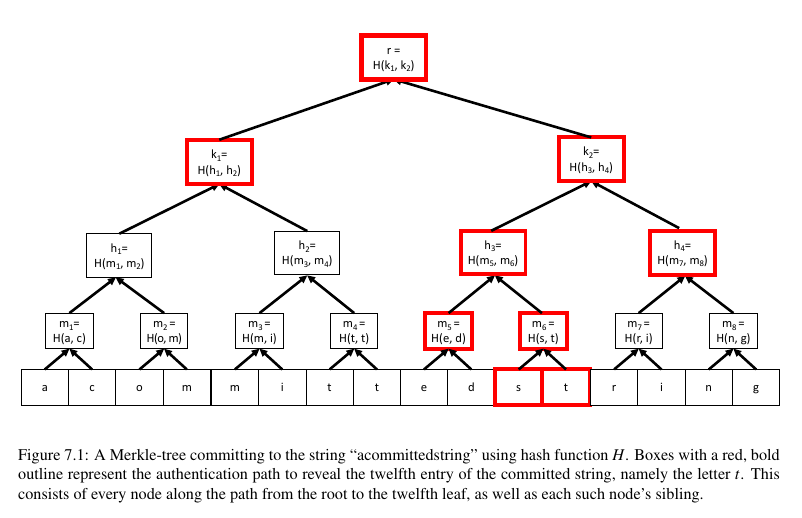
\includegraphics[scale=0.6]{merkle_tree}
\end{figure}

Unfortunately, this approach does not directly yield a polynomial commitment scheme. The committed string here could be consists of all evaluations of some totally arbitrary function, and the verifier $\mathcal{V}$ has no idea whether the string consists of all evaluations of a \textit{multilinear polynomial} as required. To address this issue, we would combine Merkle tree with a \textit{low degree test}. 

\textbf{Low-Degree tests}. Given an $m$-variate function $\widetilde{w}$ over a finite field $\F$, there are in total $\abs{\F}^m$ evaluations to make the string $s$. A low degree test only looks a tiny fraction of $s$, hence it can not determine whether $s$ is \textit{exactly} consistent with all evaluations of a low-degree polynomial (e.g., $s$ may differ from all evaluations by one value only). What the low-degree test can guarantee, is that $s$ is close to such evaluations in \textit{Hamming distance}. That is, $s$ agree with the low-degree polynomial to $\gamma$ fractions of points. 

An example of such a low-degree test is the \textit{point-versus-line} test, similar to Lemma \ref{lem:line-point}. In this test, one evaluates $s$ along a \textit{randomly chosen} line in $\F^m$, and checks that $s$ restricted to this line is consistent with a \textit{univariate polynomial} of degree at most $m$. More precisely, the verifier asks the prover for the univariate polynomial $\widetilde{w} \circ l$ for a random line $l$. Then the verifier picks a random point $r \in l$ and uses $\widetilde{w}(r)$ in the end of the GKR protocol. 

\textbf{A relaxed polynomial commitment scheme}. Combining the two techniques above, we get our first (relaxed) polynomial commitment scheme, since the committed object is close to a low-degree multilinear polynomial.

\begin{boxx1}[A first (relaxed) polynomial commitment scheme]
Let $\widetilde{w}: \F^{\log n} \rightarrow \F$ be a $\log n$-variate multilinear polynomial over $\F$. Let $s$ be the string consisting of all $\abs{\F}^{\log n}$ evaluations of $\widetilde{w}$. One obtains a polynomial commitment scheme by
\begin{itemize}
\item applying the Merkle-tree based string commitment scheme as showed above to commit to the string $s$
\item then use a low-degree test to $s$, e.g., point-versus-line test, that the verifier $\mathcal{V}$ picks a random line in $\F^{\log n}$, asks the prover $\mathcal{V}$ to check the revealed values are consistent with a univariate polynomial of degree at most $\log n$ (low-degree test), and to provide authentication information for all points along the line (binding via Merkle tree).
\end{itemize}
\end{boxx1}

If the verifier's checks in the polynomial commitment scheme pass with probability at least, say $1/2$, then the prover is bound to a string $s$ such that there is a multilinear polynomial $p$ that agree with $s$ on close to a $1/2$ fraction of points. Consequently, if a random point $r$ is not one of the "bad" points on which the string $s$ and evaluations of $\widetilde{w}$ disagree, then $\widetilde{w}(r)$ can be served in the GKR protocol as showed in the next section. 

\subsection{A First Succinct Argument for Circuit Satisfiability}

This section demonstrates our first \textit{succinct argument system} for circuit satisfiability, using the GKR protocol \textit{without} requiring the prover to explicitly send the entire $w$ to the verifier (i.e. succinctness). The can be accomplished by using the polynomial commitment scheme introduced in the last section. 

In order to check $\mathcal{C}(x, w) = y$, recall that the verifier $\mathcal{V}$ does not need to know any information whatsoever about $(x, w)$ until the very end of the protocol. $\mathcal{V}$ only needs to know $\widetilde{(x, w)}(r)$ (recall the notion of MLE from Lemma \ref{lem:MLE}) for a randomly chosen input $r$ at the end. By assumption $x$ is public, we show next it suffices to evaluate $\widetilde{w}(r)$. 

Let $z = (x, w)$, and let us assume for simplicity that $x$ and $w$ are both of length $n$, so that each entry of $z$ can be assigned a unique label in $\left\{ 0, 1 \right\}^{1 + \log n}$. Then the $i$-th entry of $x$ is assigned label $(0, i)$ while the $i$-th entry of $w$ is assigned label $(1, i)$. 

Therefore, as noticed on the GKR protocol the verifier $\mathcal{V}$ only needs to know $\tilde{z}(r_0, r_1, \dots, r_{\log n})$ at a single, randomly chosen input $r = (r_0, r_1, \dots, r_{\log n})$ at the end of the protocol. We now explain that in order to calculate $\tilde{z}(r)$, it suffices for $\mathcal{V}$ to know $\tilde{w}(r_1, \dots, r_{\log n})$. 

\begin{lemma}
To evaluate $\tilde{z}(r_0, r_1, \dots, r_{\log n})$, it suffices to evaluate $\tilde{w}(r_1, \dots, r_{\log n})$.
\end{lemma}

\begin{proof}
It is straightforward to check that
\begin{equation*}
\tilde{z}(r_0, r_1, \dots, r_{\log n}) = (1-r_0) \cdot \tilde{x}(r_1, \dots, r_{\log n}) + r_0 \cdot \tilde{w}(r_1, \dots, r_{\log n})
\end{equation*}
Indeed, the right hand side agree with $z = (x, w)$ on each label $(0, r_1, \dots r_{\log n})$ and $(1, r_1, \dots, r_{\log n})$ when $\tilde{x}$ and $\tilde{w}$ do. Also, this is a multilinear polynomial in $(r_0, \dots, r_{\log n})$. Thus, it must equal the unique multilinear extension of $z$. 
\end{proof}

\textbf{Combining polynomial commitment schemes with the GKR protocol}. When applying the GKR protocol to check $\mathcal{C}(x, w) = y$, the verifier $\mathcal{V}$ merely needs to know $\tilde{w}(r)$ for a randomly chosen input $r$ by the end of the protocol. Recall $\widetilde{w}(r)$ is exactly opening of the commitment $c$ in the polynomial commitment of the last section. Besides, since the polynomial $\widetilde{w}$ should be (implicitly) fixed at the start of the GKR protocol, So we must have the prover send the commitment $c$ to $\tilde{w}$ at the start of the protocol, e.g., the root of the Merkle tree, to the verifier. Then the prover and verifier can happily apply the GKR protocol to the claim that $\mathcal{C}(x, w) = y$, ignoring the commitment entirely until the end of the protocol. At this point, the verifier needs to know $\tilde{w}(r)$ and force the prover to reveal this quantity using commitment protocol.

\begin{boxx1}[A Succinct Argument System For Circuit SAT]
Given a circuit SAT instance $\mathcal{C}(x, w) = y$ where $x$ and $y$ are public. To apply the GKR protocol in a succinct way (without sending the whole $w$): 
\begin{itemize}
\item the prover $\mathcal{P}$ applies a polynomial commitment scheme to the polynomial $\widetilde{w}$, and get a commitment $c$ i.e. the root of the corresponding Merkle tree. 
\item the prover $\mathcal{P}$ sends the commitment $c$ to the verifier $\mathcal{V}$ to fix the polynomial $widetilde{w}$. 
\item the prover $\mathcal{P}$ and the verifier $\mathcal{V}$ simulate the roles of prover and verifier respectively in the GKR protocol and apply the protocol up to the end of the protocol. 
\item At the end of the GKR protocol, the verifier $\mathcal{V}$ takes a random point $r$ and forces the prover $\mathcal{P}$ to reveal the value $\widetilde{w}(r)$ as in the revealing phase of the commitment scheme. 
\end{itemize}

\end{boxx1}

\textbf{Cost of this succinct argument system} \colorbox{BurntOrange}{to be added}

\section{MIPs and Succinct Arguments}

\subsection{An Efficient MIP For Circuit Satisfiability} \label{sec:1st-MIP}

Multi-prover interactive proofs (MIPs) grant the verifier to access to more than one untrusted prover, and assume the provers cannot tell each other about what challenges they receive from the verifier. MIPs are important building blocks for constructing succinct arguments. 

\textbf{Non-Adaptivity}. In a single-prover interactive proof, the prover $\mathcal{P}$ is allowed to act \textit{adaptively} in the sense that $\mathcal{P}$'s response to the $i$-th message $m_i$ sent from $\mathcal{V}$ is allowed to depend on the preceding $i-1$ messages. Thus, the presence of a second prover who doesn't know $\mathcal{V}$'s messages to the first prover, prevents the first prover from behaving in adaptive manner. 

Next, we will show the \textit{succinctness} brought by the non-adaptivity. Recall the polynomial commitment scheme enforced non-adaptivity, i.e., the prover $\mathcal{P}$ must tell $\mathcal{V}$ with $\tilde{w}(r)$, and is not able to change its answer based on the interaction with $\mathcal{V}$. The addition of a second prover in a $2$-prover MIP has exactly the same effect. 

Let $\mathcal{C}$ be an arithmetic circuit over a field $\F$ taking an explicit input $x$ and a non-deterministic input $w$. Let $S = 2^k$ denote the number of gates in $\mathcal{C}$, and assign each gate in $\mathcal{C}$ a binary label in $\left\{ 0, 1 \right\}^k$. 

\textbf{Transcript}. An assignment of values to each gate of $\mathcal{C}$ is called a \textit{transcript} of $\mathcal{C}$ and such a transcript can be viewed as a function
\begin{equation*}
W: \left\{ 0, 1 \right\}^k \rightarrow \F
\end{equation*}

Given a claim that $\mathcal{C}(x, w) = y$, a \textit{correct transcript} is a transcript satisfying this circuit. See the figure below. 
\begin{figure}[h] \label{fig:circuit-transcript}
\centering
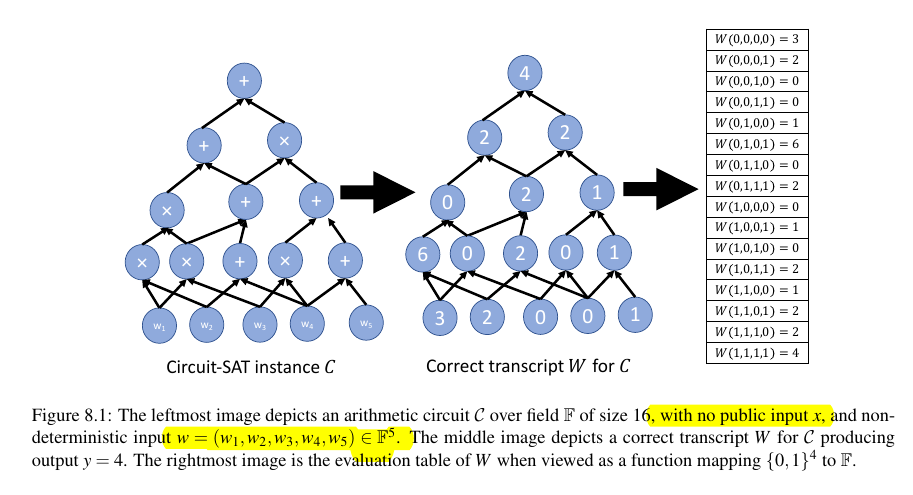
\includegraphics[scale=0.6]{correct_transcript}
\end{figure}

\textbf{Functions}. The MIP works by having the first prover $\mathcal{P}_1$ claim to hold a polynomial function $Z$ as an extension (not necessarily MLE) of a correct transcript $W$ for $\left\{ \mathcal{C}, x, y \right\}$. If the prover is honest, say $Z = \widetilde{W}$ the MLE of $W$ (in later chapter we will see $Z$ could be other extension polynomial function). We shall establish a polynomial
\begin{equation*}
g_{x, y, Z}: \F^{3k} \rightarrow \F
\end{equation*}

satisfying 

\begin{equation*}
\forall (a, b, c) \in \left\{ 0, 1 \right\}^{3k} \: g_{x, y, Z}(a, b, c) = 0 \Longleftrightarrow Z = \widetilde{W}
\end{equation*}

\begin{enumerate}
\item\label{item:52} First we denote the following functions (all $x$ is \textit{simply} viewed as the input of the circuit):
\begin{equation*}
\text{add, mult}: \left\{ 0, 1 \right\}^{3k} \rightarrow \left\{ 0, 1 \right\}
\end{equation*}
that take as input three gate labels $(a, b, c)$ from $\mathcal{C}$ and outputs $1$ iff gate $a$ adds (respectively, multiplies) the outputs of gates $b$ and $c$. 
\item\label{item:53} 
\begin{equation*}
\text{io}: \left\{ 0, 1 \right\}^{3k} \rightarrow \left\{ 0, 1 \right\}
\end{equation*}
returns $1$ when gate $a$ is either a gate from input or one of the output gate, and gates $b$ and $c$ are the in-neighbors of $a$ (input gates have in-neighbors $b = c = 0$). 
\item\label{item:54} Fix the input $x$ and output $y$, the next function returns the input and output values depending on the given label:
\begin{equation*}
I_{x, y}: \left\{ 0, 1 \right\}^k \rightarrow \F
\end{equation*}
such that $I_{x, y}(a) = x_{a}$ if $a$ is the label of an input gate, $I_{x, y}(a) = y_a$ if $a$ is the label of an output gate, and $I_{x, y}(a) = 0$ otherwise.
\end{enumerate}

\begin{lemma}
Given the circuit $\mathcal{C}(x) = y$ with transcript $W$, define the function
\begin{equation*}
G_{x, y, W}(a, b, c) = \text{io}(a, b, c) \cdot (I_{x, y}(a) - W(a)) + \text{add}(a, b, c) \cdot (W(a) - (W(b) + W(c))) + \text{mult}(a, b, c) \cdot (W(a) - W(b) \cdot W(c))
\end{equation*}
$G_{x, y, W}(a, b, c) = 0$ for all $(a, b, c) \in \left\{ 0, 1 \right\}^{3k}$ iff $W$ is a correct transcript for $\left\{ C, x, y \right\}$.
\end{lemma}

\begin{proof}
Based on the gate $a$ as being input, output or internal gate, many terms in the last function would be eliminated. 
\end{proof}

Now replace the correct transcript $W$ by \textit{any polynomial function} in the form $Z: \F^k \rightarrow \F$, define the polynomial
\begin{equation*}
g_{x, y, Z}(a, b, c) =  \widetilde{\text{io}}(a, b, c) \cdot (\widetilde{I}_{x, y}(a) - Z(a)) + \widetilde{\text{add}}(a, b, c) \cdot (Z(a) - (Z(b) + Z(c))) + \widetilde{\text{mult}}(a, b, c) \cdot (Z(a) - Z(b) \cdot Z(c))
\end{equation*}
Thus by the above lemma, $Z$ extends a correct transcript $W$ (even $Z$ is not a MLE) iff $g_{x, y Z}$ vanishes on all $(a, b, c) \in \left\{ 0, 1 \right\}^{3k}$.

\textbf{Identifier function $\beta_{3k}(a, b)$}. The bit-wise identifier function is defined by 
\begin{equation*}
\beta_{3k}(a, b): \left\{ 0, 1 \right\}^{3k} \times \left\{ 0, 1 \right\}^{3k} \rightarrow \left\{ 0, 1 \right\}
\end{equation*}
be the function that returns $1$ iff $a = b \in \left\{ 0, 1 \right\}^{3k}$. It is easy to construct its MLE
\begin{equation} \label{eq:identifier}
\widetilde{\beta}_{3k}(a, b) = \prod_{j = 1}^{3k} \left( (1 - a_j) (1 - b_j) + a_jb_j \right)
\end{equation}
Consider the polynomial
\begin{equation*}
p(X) = \sum_{u \in \left\{ 0, 1 \right\}^{3k}} \widetilde{\beta}_{3k}(X, u) \cdot g_{x, y, Z}(u)
\end{equation*}
Note that $p$ is multilinear in $X$ and $p(a, b, c) = 0$ for all $(a, b, c) \in \left\{ 0, 1 \right\}^{3k}$ iff $g_{x, y, Z}$ does. Recall the MLE is \textit{unique}, thus $p$ is \textit{identically zero polynomial} iff $g_{x, y, Z}$ vanishes over $\left\{ 0, 1 \right\}^{3k}$. 

For the verifier $\mathcal{V}$ to check $p$ is indeed the zero-polynomial, as usual $\mathcal{V}$ picks a random input $r \in \left\{ 0, 1 \right\}^{3k}$ and confirm that $p(r) = 0$. By the Schwarts-Zippel lemma \ref{lem:multivariate-root-portion}, the probability of $p$ is non-zero with $p(r) = 0$ is at most $d/\abs{\F}$.

\textbf{Application of the sum-check protocol}. For the verifier $\mathcal{V}$ to check 
\begin{equation} \label{eq:identifier-sum-check}
p(r) = \sum_{u \in \left\{ 0, 1 \right\}^{3k}} \widetilde{\beta}_{3k}(r, u) \cdot g_{x, y, Z}(u) = 0
\end{equation}
We define
\begin{equation*}
h_{x, y, Z}(Y) = \widetilde{\beta}_{3k}(r, Y) \cdot g_{x, y, Z}(Y)
\end{equation*}
such that 
\begin{equation*}
p(r) = \sum_{u \in \left\{ 0, 1 \right\}^{3k}} h_{x, y, Z}(u)
\end{equation*}
Thus, $\mathcal{V}$ applies the sum-check protocol to $h_{x, y, Z}$ with the first prover $\mathcal{P}_1$ playing the role in this protocol. To perform the final check in the sum-check protocol, $\mathcal{V}$ needs to evaluate $h_{x, y, Z}$ at a random point $r' \in \F^{3k}$. Let $r_1', r_2'$ and $r_3'$ denote the first, second and third $k$ entries of $r'$. Then evaluating $h_{x, y, Z}(r')$ of $\mathcal{V}$ requires evaluations about $\widetilde{\text{io}}(r'), \widetilde{\text{add}}(r'), \widetilde{\text{mult}}(r'), \widetilde{I}_{x, y}(r_1'), Z(r_1'), Z(r_2'), Z(r_3')$. However, $\mathcal{V}$ can not evaluate $Z(r_1'), Z(r_2'), Z(r_3')$ without help of $\mathcal{P}_1$, since $\mathcal{V}$ does not know $Z$. We show in the following how MIP solves this problem.

\textbf{A MIP for circuit SAT}. To deal with this problem, we use the same trick of reducing multiple points to one: let $l$ be a canonical \textit{degree-two} curve passing through $r_1', r_2'$ and $r_3'$ such that $l(0) = r_1', l(1) = r_2'$ and $l(2) = r_3'$. Then the verifier $\mathcal{V}$ asks the first prover $\mathcal{P}_1$ for the \textit{univariate} polynomial $Z \circ l$. To verify the authenticity, $\mathcal{V}$ must pick another random $r'_4 \in l$ and to check $Z(r'_4)$. Still, $\mathcal{V}$ has no idea about this value, this is where the second prover $\mathcal{P}_2$ comes into play. As in the \textit{The Low-Degree test}, $\mathcal{V}$ sends $\mathcal{P}_2$ a \textit{random} line $l'$ in $\F^k$ passing through $r'_{4}$, and demands $\mathcal{P}_2$ reply with a univariate polynomial of degree at most $k$, claimed to equal $Z \circ l'$. Note that $\mathcal{P}_2$ doesn't know which point in $l'$ equals $r'_4$. $\mathcal{P}_2$'s response implicitly specifies a value for $Z(r'_{4})$. $\mathcal{V}$ accepts if this value equals the evaluation of the univariate polynomial $Z \circ l$ claimed by $\mathcal{P}_1$ and rejects otherwise.  

\textit{Comparison to the GKR Protocol}. Recall the GKR protocol is for the circuit SAT problem while using polynomials and their evaluations to represent the values of the circuit as well. However, the GKR protocol verifies the claim $\mathcal{C}(x, w) = y$ \textit{layer by layer} with the sum-check protocol applied to each layer. In constrast, this MIP protocol verifies the whole circuit in one shot, using \textit{a single} invocation of the sum-check protocol. 

The reason is that the verifier only has access to the input value or the lowest layer of the circuit, since the verifier never materializes the intermediate gate. On the other hand, in the MIP, the first prover $\mathcal{P}_1$ makes a claim about the entire transcript, even $\mathcal{V}$ cannot check this independently, but the second prover $\mathcal{P}_2$ may come to help. 

\subsection{Extension from Circuit-SAT to R1CS-SAT}

\begin{boxx1}[Rank-$1$ Constraint System (R1CS)]
A rank-$1$ constraint system (R1CS) instance (also referred to as Quadratic Arithmetic Programs (QAPs)) is specified by three $m \times n$ matrices $A, B$ and $C$ with entries from a field $\F$ and is satisfiable iff there is a vector $z \in \F^n$ such that 

\begin{equation} \label{eq:r1cs}
(A \cdot z) \circ (B \cdot z) = C \cdot z
\end{equation}

where $\cdot$ denotes matrix-vector product, and $\circ$ denotes entrywise product. Any vector $z$ satisfying this equation is analogous to the notion of a correct transcript in the context of arithmetic circuit satisfiability. 

\end{boxx1}

\textbf{R1CS-SAT and Arithmetic Circuit-SAT}. The R1CS-SAT problem can be thought of as a generalization of the Arithmetic Circuit-SAT problem in the following sense: any instance of Arithmetic Circuit-SAT can be efficiently transformed into instances of R1CS-SAT. Consider an instance $\left\{ \mathcal{C}, x, y \right\}$ of arithmetic circuit-SAT where the prover wants to convince the verifier that there is a $w$ such that
\begin{equation*}
\mathcal{C}(x, w) = y
\end{equation*}
We may consider $(x, w)$ as the input while $(w)$ is secret. We need to construct matrices $A, B, C$ such that there exists a vector $z$ satisfying the above equation. 

Let $N$ be the sum of the lengths of $x, y$ and $w$, plus the number of gates. In other words, the $N$-dimensional vector can hold all labels regarding the above quantities: $(x_1, \dots, x_m, w_1, \dots, w_n, y_1, \dots, y_l, ad_1, \dots, mul_1, \dots)$. And let $M = N - \abs{w}$. The R1CS-SAT instance will consists of three $M \times (N+1)$ matrices $A, B, C$, where $N$ be the sum of the lengths of $x, y$ and $w$, plus the number of gates in $\mathcal{C}$, and let $M = N - \abs{w}$. We will fix the first entry $z_1 = 1$ of the vector $z$, and associate each remaining entry of $z$ with either an entry of $x, y$ or $w$, or a gate of $\mathcal{C}$, that explains the dimension $(N + 1)$. On the other hand, the above equation (\ref{eq:r1cs}) gives $M$ relations following each the rows of matrices, and every relation indicates one \textit{constraint} for $x, y$ and intermediate gates, since there is no constraint for the witness $w$ considering it is not public. Next, we define the matrices in order to explicitly form the constraints in the following way:

\begin{enumerate}
\item\label{item:55} For the $j$-th entry of $z$ that corresponds to $x_i$ of $x$, we define the $j$-th row of $A$ to be the standard basis vector $e_1 \in \F^{N+1}$ to make the $j$-th coordinate as $1$, the $j$-th row of $B$ to be the standard basis vector $e_j \in \F^{N+1}$ to make the $j$-th coordinate as $z_{j}$ and the $j$-th row of $C$ to be the standard basis vector $x_i \cdot e_{1} \in \F^{N+1}$ to make the $j$-th coordinate as $x_{i}$. Consequently, this row gives exactly the left side along with the right side:

\begin{equation*}
1 \cdot z_{j} = x_{i} 
\end{equation*} 
\item\label{item:56} For the $j$-th entry of $z$ that corresponds to an addition gate of $\mathcal{C}$ that adds $z$'s entries indexed by $j', j''$, we set the $j$-th row of $A$ to be $e_1 \in \F^{N+1}$, the $j$-th row of $B$ to be $e_{j'} + e_{j''} \in \F^{N+1}$, and the $j$-th row of $C$ to be $e_{j}$. Then the row gives left side with the right side:

\begin{equation*}
1 \cdot (z_{j'} + z_{j''}) = z_j
\end{equation*}
\item\label{item:57} For the $j$-th entry of $z$ that corresponds to a multiplication gate of $C$ that multiplies $z$'s entries indexed by $j', j''$, we set the $j$-th row of $A$ to be $e_{j'} \in \F^{N+1}$, the $j$-th row of $B$ to be $e_{j''} \in \F^{N+1}$, and the $j$-th row of $C$ to be $e_{j}$. Then the row gives left side with the right side:

\begin{equation*}
z_{j'} \cdot z_{j''} = z_j
\end{equation*}
\end{enumerate}

\textbf{Remark}. See the following figure, we assume the only input is the secret witness $w$, the when translated in the constraints, there are constraints about addition or multiplication gates, output gates. However, no constraint about the input gates.
\begin{figure}[H]
\centering
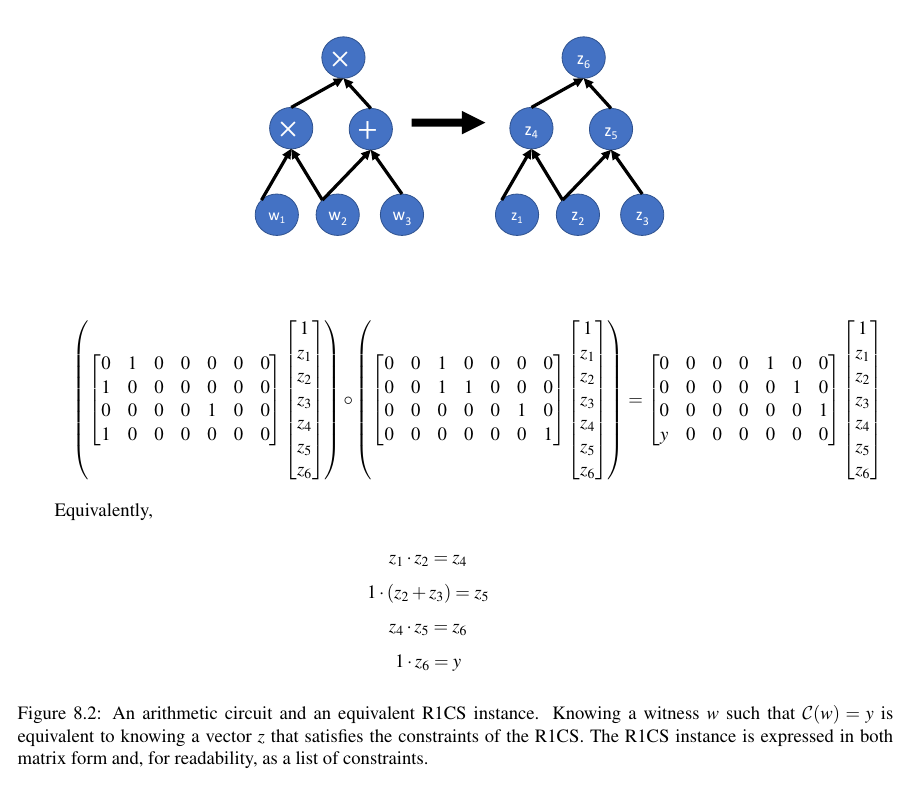
\includegraphics[scale=0.5]{R1CS}
\end{figure}

\textbf{An MIP for R1CS-SAT}. View the matrices $A, B$ and $C$ as functions 
\begin{equation*}
f_A, f_B, f_C: \left\{ 0, 1 \right\}^{\log_2 M} \times \left\{ 0, 1 \right\}^{\log_2 N+1} \rightarrow \F
\end{equation*}
and 
\begin{equation*}
Z: \left\{ 0, 1 \right\}^{\log_2(N+1)} \rightarrow \F
\end{equation*}

Then the above equation (\ref{eq:r1cs}) becomes: for all row index $a \in \left\{ 0, 1 \right\}^{\log_2(M)}$ we have the equality: 

\begin{equation} \label{eq:r1cs-2}
\left( \sum_{b \in \left\{ 0, 1 \right\}^{\log_2(N+1)}} \widetilde{f}_A(a, b) \cdot Z(b) \right) \cdot \left( \sum_{b \in \left\{ 0, 1 \right\}^{\log_2(N+1)}} \widetilde{f}_{B}(a, b) \cdot Z(b) \right) = \left( \sum_{b \in \left\{ 0, 1 \right\}^{\log_2(N+1)}} \widetilde{f}_{C}(a, b) \cdot Z(b) \right)
\end{equation}

Let $g_Z$ denote the $\log_2(M)$-variate polynomial over the row index:
\begin{equation*}
g_Z(X) = \left( \sum_{b \in \left\{ 0, 1 \right\}^{\log_2(N+1)}} \widetilde{f}_A(X, b) \cdot Z(b) \right) \cdot \left( \sum_{b \in \left\{ 0, 1 \right\}^{\log_2(N+1)}} \widetilde{f}_{B}(X, b) \cdot Z(b) \right) - \left( \sum_{b \in \left\{ 0, 1 \right\}^{\log_2(N+1)}} \widetilde{f}_{C}(X, b) \cdot Z(b) \right)
\end{equation*}
The polynomial has degree at most $2$ in each variable and the above equation (\ref{eq:r1cs-2}) holds iff $g_Z$ vanishes at all inputs in $\left\{ 0, 1 \right\}^{\log_2(M)}$.

Similar to (\ref{eq:identifier-sum-check}) we use the identifier $\widetilde{\beta}(a, b)$ as in (\ref{eq:identifier}) and define

\begin{equation*}
p(Y) = \sum_{u \in \left\{ 0, 1 \right\}^{\log_2 (M)}}  \widetilde{\beta}_{\log_2 M}(Y, u) \cdot g_Z(u)
\end{equation*}
Since $p(Y) = 0$ for all $Y \in \left\{ 0, 1 \right\}^{\log_2(M)}$ and $p(Y)$ is MLE, $p(Y)$ is zero-polynomial. Taking a random $r$, thus 
\begin{equation*}
p(r) = \sum_{u \in \left\{ 0, 1 \right\}^{\log_2 (M)}}  \widetilde{\beta}_{\log_2 M}(r, u) \cdot g_Z(u) = 0
\end{equation*}
Therefore, to apply the sum-check protocol we define
\begin{equation*}
h_Z(T) = \widetilde{\beta}_{\log_2 M}(r, T) \cdot g_Z(T)
\end{equation*}
The verifier $\mathcal{V}$ needs to evaluate $h_Z(T)$ at a random input $r' \in \F^{\log_2(M)}$. Considering $\mathcal{V}$ is able to evaluate $\widetilde{\beta}_{\log_2 M}(r, r')$ without help, it is enough to deal with the evaluation of $g_Z(r')$. More precisely,

\begin{equation*}
g_Z(r') =  \left( \sum_{b \in \left\{ 0, 1 \right\}^{\log_2(N+1)}} \widetilde{f}_A(r', b) \cdot Z(b) \right) \cdot \left( \sum_{b \in \left\{ 0, 1 \right\}^{\log_2(N+1)}} \widetilde{f}_{B}(r', b) \cdot Z(b) \right) - \left( \sum_{b \in \left\{ 0, 1 \right\}^{\log_2(N+1)}} \widetilde{f}_{C}(r', b) \cdot Z(b) \right)
\end{equation*} 


This means that to compute $g_Z(r')$, it suffices to apply the sum-check protocol three more times, to the following three $\log_2 (N+1)$-variate polynomials:
\begin{equation*}
\begin{split}
& p_1(X) =  \widetilde{f}_A(r', X) \cdot Z(X) \\
& p_2(X) =  \widetilde{f}_{B}(r', X) \cdot Z(X) \\
& p_3(X) =  \widetilde{f}_{C}(r', X) \cdot Z(X)
\end{split}
\end{equation*}
Note that all three invocations of sum-check can be executed in parallel. At the end of these three final invocations of the sum-check protocol, the verifier $\mathcal{V}$ needs to evaluate each of $p_1, p_2$ and $p_3$ at a random input $r''$. Similarly, only the evaluation of $Z(r'')$ poses problem. At this point, the situation is exactly analogous to the MIP for arithmetic circuit-SAT of last section, $Z(r'')$ can be obtained from the second prover $\mathcal{P}_2$ using a low-degree test. 

\colorbox{BurntOrange}{TODO: runtime analysis}

\section{Interactive Oracle Proofs}

\subsection{Polynomials IOPs and Associated Succinct Arguments}

\begin{boxx1}[Interactive Oracle Proofs]
An interactive oracle proof (IOP) is an IP where, in each round the verifier is not forced to read the prover's entire message, but rather is given query access to the message so that the verifier can choose to look at any desired symbol of the message.
\end{boxx1}

Let's call the messages in an IOP as special messages since oracle access is attached to each of them. In a \textit{polynomial IOP}, rather than normal string, each special message $i$ specifies a \textit{polynomial} $h_i$ (e.g., via its evaluations) over a field $\F$ with degree at most $d_i$. Here $h_i$ is considered as \textit{univariate}, but in general $h_i$ may be a multivariate polynomial. 

Think of $h_i$ as having a very large degree or number of coefficients, in fact, normally the degree $d_i$ may be as large as the entire R1CS instance. Consequently, the verifier $\mathcal{V}$ is given query access to evaluations of $h_i$ such that $\mathcal{V}$ can choose any input $r$ to learn $h_i(r)$. 

\subsection{The Univariate Sum-Check Protocol over A Multiplicative Group}

Recall the Sum-Check protocol (\ref{eq:sum-check-protocol}) is for \textit{multivariate polynomial} over the Boolean hypercube $\left\{ 0, 1 \right\}^{\log S}$. Here we study the cases for any low-degree \textit{univariate polynomial} defined over a multiplicative subgroup $H$ of the field $\F$. 

\begin{lemma}
Let $\F$ be a finite field and suppose $H$ is a multiplicative subgroup of $\F$ with size $\abs{H} = n$. Then for any univariate polynomial $q$ of degree less than $n$, we have
\begin{equation*}
\sum_{h \in H} q(h) = q(0) \cdot \abs{H}
\end{equation*}
Hence, $\sum \limits_{h \in H} q(a) = 0$ iff $q(0) = 0$.
\end{lemma}

\begin{proof}
Notice $H$ is cyclic and all elements in $H$ are exactly the roots of $X^{n} - 1$, define the univariate degree-$n$ polynomial
\begin{equation*}
Z_H(X) = \prod_{h \in H} (X - h) = X^n - 1
\end{equation*}

where follows $\sum \limits_{h \in H} h = 0$. It suffices to prove $\sum \limits_{h \in H} h^m = 0$ for any nonzero power $m < n$, which can be found easily using any generator of $H$.
\end{proof}

Applying euclidean division over $\F[X]$ and the above lemma, we can easily deduce the following result 

\begin{lemma}
For any polynomial $p(X)$ with degree $D$, the two following are equivalent: 
\begin{itemize}
\item $\sum \limits_{h \in H} p(h) = 0$ 
\item there exists polynomial $h^{\displaystyle *}$ with degree at most $D-n$ and $f$ with degree at most $n-1$ such that 
\begin{equation*}
p(X) = h^{\displaystyle *}(X) \cdot Z_H(X) + X \cdot f(X)
\end{equation*}
\end{itemize}
\end{lemma}

\textbf{The univariate sum-check protocol}. To verify the sum $\sum \limits_{h \in H} p(h) = 0$, it is sufficient
\begin{enumerate}
\item\label{item:108} the prover $\mathcal{P}$ establishes that there exists functions $h^{\displaystyle *}$ and $f$ such that the above equation holds, by sending the corresponding special messages (or their commitments) to the verifier 
\item\label{item:109} the verifier $\mathcal{V}$ can use the query access to evaluate the above equation (since all $p, h^{\displaystyle *}, f$ are available) at a random point $r \in \F$. It is easy to see the soundness error is up to $\max\{D, n\} / \F$:
\begin{equation*}
p(r) = h^{\displaystyle *}(r) \cdot Z_H(r) + r \cdot f(r)
\end{equation*}
\end{enumerate}

\subsection{A Polynomial IOP for R1CS-SAT}

Recall given an arithmetic circuit-SAT instance $\mathcal{C}(x, w) = y$ where the circuit input is the pair $(x, w)$ while the witness $w$ is only known to the prover $\mathcal{P}$. Then all values of $x, w$ and $y$ as well as intermediate gates values (also called \textit{correct transcript} of the circuit) can be represented in the vector $z$, also the circuit can be interpreted in constraints by matrices $A, B$ and $C$ in $M_{M \times (N+1)}(\F)$ satisfying
\begin{equation*}
(A \cdot z) \circ (B \cdot z) = C \cdot z
\end{equation*}
where the $M$ rows demonstrate relations about public input and output as well as each arithmetic gates. The protocol of \textit{R1CS-SAT} basically asks the prover and the verifier to check the validity of the last equality. 

Now suppose the dimensions of the matrices $M = N+1 = n$ and a multiplicative subgroup $H$ of $\F$ is with the size $\abs{H} = n$ as well. Hence, the vector $z$ can be \textit{indexed} via $H$ as
\begin{equation*}
z = \left( z_h \right)_{h \in H}
\end{equation*}
Recall the $n$-dimensional vector $z$ can be identified with the degree $n-1$ univariate polynomial $\widetilde{z}$ using \textit{Lagrange Interpolation} (\ref{eq:univariate-lagrange}) such that for all $h \in H$:
\begin{equation*}
\widetilde{z}(h) = z_{h}
\end{equation*}
Similarly, for the vectors $z_A = Az, z_B = Bz$ and $z_C = Cz$ in $\F^n$ we denote the univariate polynomials $\widetilde{z}_A, \widetilde{z}_B$ and $\widetilde{z}_C$ as their extensions. Now the constraints become: for all $h \in H$
\begin{equation*}
\begin{cases}
\widetilde{z}_A(h) \cdot \widetilde{z}_{B}(h) = \widetilde{z}_C(h) \\
\widetilde{z}_M(h) = \sum \limits_{j \in H} M_{h, j} \cdot \widetilde{z}(j) \text{ for } M \in \left\{ A, B, C \right\} 
\end{cases}
\end{equation*}

\textbf{Checking the 1st Equation}. Since it can be viewed as a polynomial function vanishing over $H$ and $\Z_H(X) = \prod_{h \in H}(X - h)$, there exists a polynomial $h^{\displaystyle *}$ with degree $\leq n$ such that
\begin{equation*}
\widetilde{z}_A(X) \cdot \widetilde{z}_{B}(X) - \widetilde{z}_C(X) = h^{\displaystyle *} (X) \cdot \Z_H(X)
\end{equation*}
 
Therefore, it suffices for the prover $\mathcal{P}$ to send a \textit{special message} (i.e the commitment) specifying the polynomial $h^{\displaystyle *}$. Then the verifier picks a random $r \in \F$ and checks 
\begin{equation*}
\widetilde{z}_A(r) \cdot \widetilde{z}_{B}(r) - \widetilde{z}_C(r) = h^{\displaystyle *} (r) \cdot \Z_H(r)
\end{equation*}

Note the degrees of all involved polynomials are at most $2n$, thus the soundness error is at most $2n / \abs{\F}$.

\textbf{Checking the 2nd Equation}. Fix the matrix $M \in \left\{ A, B, C \right\}$. To check the $2$nd equation, we should find a polynomial of representing the matrix $M$. As the rows and columns are indexed by $H$, we encode $M$ as a function 
\begin{equation*}
\begin{split}
M: H \times H & \rightarrow \F \\
M(x, y) & = M_{x, y}
\end{split}
\end{equation*}
Next, we introduce a \textit{bivariate low-degree} extension $\widetilde{M}(X, Y)$ of the matrix $M$ with degree at most $n - 1$ in each variable. First, as the identifier introduced in (\ref{eq:identifier}) used to identify the case of two identical inputs, we define a bivariate polynomial (recall $\abs{H} = n$) as following
\begin{equation*}
u_H(X, Y) = \frac{X^n - Y^n}{X - Y} = X^{n-1} + X^{n-2}Y + X^{n-3}Y^2 + \cdots + XY^{n-2} + Y^{n-1}
\end{equation*}
\begin{itemize}
\item For $x, y \in H$ with $x \neq y$, $u_H(x, y) = 0$, as $x^n = y^n = 1$ and we use the expression of the fraction.
\item For all $x \in H$, $u_H(x, x) = nx^{n-1} \neq 0 \in \F$.
\end{itemize}

Besides, depending on the matrix $M$ being sparse or dense, choose a multiplicative subgroup $\mathcal{K}$ with order $K$ of the field $\F$ and establish a bijection between the \textit{nonzero entries} of $M$ and $\mathcal{K}$. By this identification, we define the getting-index-row and getting-index-column functions for each nonzero entry of $M$:
\begin{equation*}
\text{row, col: } \mathcal{K} \simeq M \rightarrow H \subset \F
\end{equation*}
and the value function:
\begin{equation*}
\begin{split}
\text{val: } \mathcal{K}  & \simeq M  \rightarrow \F \\
 k & \mapsto M_{i, j}  \mapsto M_{i, j} / \left( u_H(\text{row} (k), \text{row}(k)) \cdot u_H(\text{col} (k), \text{col}(k)) \right)
\end{split}
\end{equation*}
Using Lagrange Interpolation, all three functions can be extended into \textit{univariate polynomials} $\widetilde{\text{val}}, \widetilde{\text{row}}$ and $\widetilde{\text{col}}$ of degree at most $K$. Then we can express
\begin{equation*}
\widetilde{M}(X, Y) = \sum_{k \in \mathcal{K}} u_H(X, \widetilde{\text{row}}(k)) \cdot u_H(Y, \widetilde{\text{col}}(k)) \cdot \widetilde{\text{val}}(k)
\end{equation*}
It is apparent that $\widetilde{M}$ agrees with the matrix $M$ at all \textit{non-zero} entries of index in $\mathcal{K} \subset H \times H$. Also, the bivariate polynomial $\widetilde{M}(X, Y)$ has degree at most $n-1$ in both $X$ and $Y$, thus as polynomials in $\F^{\leq n - 1} [X]$ the following equality follows
\begin{equation*}
\widetilde{z}_M(X) = \sum_{j \in H} \widetilde{M}(X, j) \widetilde{z}(j)
\end{equation*}
since both polynomials of the two sides have the same values over the $n$ elements in $H \subset \F$, then the second equation follows.
 
As usual, the verifier picks a random $r' \in \F$, then up to soundness error $n/\abs{\F}$, the equation holds iff 
\begin{equation*}
\widetilde{z}_M(r') = \sum_{j \in H} \widetilde{M}(r', j) \widetilde{z}(j)
\end{equation*}
As analogy to the formal R1CS, we can use (univariate) sum-check protocol to verify this sum. Let
\begin{equation*}
q(Y) = \widetilde{M}(r', Y) \widetilde{z}(Y) - \widetilde{z}_M(r') \cdot \abs{H}^{-1}
\end{equation*}
be the degree $n-1$ polynomial. Thus the above equality becomes
\begin{equation*}
\sum_{j \in H} q(j) = 0
\end{equation*}
where the univariate sum-check protocol of the last section can be applied to $q(Y)$ by the verifier.

\subsection{Several Gadgets of Plonkish IOPs} \label{sec:sever-gadg-plonk}

Recall we have introduced the \textit{Sum-Check} argument (of knowledge) for any univariate polynomial over a cyclic multiplicative subgroup $H \subset \F^{\displaystyle *}$. In this section, we will study more \textit{univariate} polynomial IOPs used in Plonk proof system based on the great slides \cite{boneh2023zkmooc} of Dan Boneh. Recall the \textit{vanishing polynomial over $H$} is defined by the degree $n$ univariate polynomial:

\begin{equation*}
Z_H(X) = \prod_{i = 0}^{n-1} (X - \omega^i) = X^n - 1
\end{equation*}

\textbf{Zero-Check Argument}. See Dan's slides.

\textbf{Product-Check Argument}. See Dan's slides. Notice that here the \textit{running product} polynomial $t(X) \in \F^{< n} [X]$ (I use the rank $n$ instead of $k$ as in the slides) to help prove 
\begin{equation*}
\prod_H f(\omega^{i}) = 1
\end{equation*}
is the interpolation polynomial of the pairs 
\begin{equation*}
\left\{ (\omega^i, u_i) \right\}_{i = 0, \dots, n-1} \quad \text{ for } \mathbf{u} = (u_{0}, \dots, u_{n-1}) \text{ is the vector to be encoded}
\end{equation*}
Thus $t(X)$ is defined by
\begin{equation*}
t(\omega^{i}) = 
\begin{cases}
f(1)  & \text{ for } i = 0 \\
\prod_{i = 0}^s f(\omega^s) & \text{ for } i = 1, \dots, n-1
\end{cases}
\end{equation*}
Thus the argument of $\prod f(\omega^i) = 1$ can be reduced to the \textit{Zero-Check} argument 
\begin{equation} \label{eq:product-check}
\begin{cases}
t(\omega \cdot X) - t(X) f(\omega \cdot X) = 0 \text{ over } H \\
t(\omega^{n-1}) = 1
\end{cases}
\end{equation}
\begin{remark}
When $X = \omega^{n-1}$ the above relation still holds, as
\begin{equation*}
t(1) - t(\omega^{n-1}) f(1) = t(1) - f(1) = 0
\end{equation*}
Thus, it is well defined as Zero-Check argument over the whole $H$.
\end{remark}

\textbf{Permutation-Check Argument} (Multiset-Check in some literature and the pre-defined permutation is called Permutation-Check). See Dan's slides. The essential idea is that we construct two polynomials using the two lists $\left\{ f(\omega^i) \right\}, \left\{ g(\omega^i) \right\}$:
\begin{equation*}
\begin{cases}
F(X) = \prod_{i = 0}^{n-1} (X - f(\omega^i)) \\
G(X) = \prod_{i = 0}^{n-1} (X - g(\omega^i))
\end{cases}
\end{equation*}
As usual, to prove \textit{equality of polynomial} we evaluate at random point $r$ and we try to prove
\begin{equation*}
\prod_{i = 0}^{n-1} \frac{r - f(\omega^i)}{r - g(\omega^i)} = 1
\end{equation*}
Then we apply the Product-Check argument to the rational function $\frac{r - f(X)}{r - g(X)}$ (it still works for rational functions) by using
\begin{equation*}
\begin{cases}
t(\omega \cdot X) (r - g(\omega \cdot X)) - t(X) (r - f(\omega \cdot X)) = 0 \text{ over } H\\
t(\omega^{n-1}) = 1
\end{cases}
\end{equation*}

\textbf{Pre-defined Permutation-Check Argument}. For two polynomial functions:
\begin{equation*}
f, g: \F \longrightarrow \F
\end{equation*}
and another permutation over the subgroup $H \subset \F^{\displaystyle *}$
\begin{equation*}
\sigma: H \longrightarrow H
\end{equation*}
Suppose $f$ and $g$ satisfy the relation:
\begin{equation} \label{eq:permuation-composite}
g(\sigma(\omega^i)) = f(\omega^i) \text{ for } i = 0, \dots, n-1
\end{equation}
In other words, $f$ equals the composite function $g \circ \sigma$ over $H$. A good example is the interpolation polynomial $g$ under the \textit{Wiring identity}. More precisely, $g$ is defined by the list of pairs:
\begin{equation*}
\left\{ (\omega^i, u_i) \right\}_{i = 0, \dots, n-1}
\end{equation*}
and the Wiring Identity requires:
\begin{equation*}
u_{\sigma_i} = u_i \quad \text{ where } \sigma_{i} \text{ is the index of } \sigma(\omega^i) = \omega^{\sigma_i} 
\end{equation*}
It is easy to check that $g$ satisfies the above relation (\ref{eq:permuation-composite}) as
\begin{equation*}
g(\sigma(\omega^i)) = g(\omega^{\sigma_i}) = g(\omega^i) \quad \text{ for } i = 0, \dots, n-1
\end{equation*}
Now, the statement that $f = g \circ \sigma$ over $H$ is equivalent to the fact that the following two lists 
\begin{equation*}
\begin{cases}
\left\{ (\omega^i, g(\omega^i)) \right\}_{i = 0, \dots, n-1} \\
\left\{ \left( \sigma(\omega^i), f(\omega^i) = g(\sigma(\omega^i)) \right) \right\}_{i = 0, \dots, n-1}
\end{cases}
\end{equation*}
are permutation from one to the other (note that $f_0 = g_{\sigma_0}$). Therefore, we construct the following two \textit{bi-variate} polynomials in $\F[X, Y]$:
\begin{equation*}
\begin{cases}
F(X, Y) = \prod_{i = 0}^{n-1} (X - Y \cdot \omega^i - g(\omega^i)) \\
G(X, Y) = \prod_{i = 0}^{n-1} (X - Y \cdot \sigma(\omega^i) - f(\omega^i)) 
\end{cases}
\end{equation*}
(Note that Plonk use the pairs $(i, g(\omega^i))$ directly instead of $(\omega^i, g(\omega^i))$) Based on the fact that $\F[X, Y]$ is UFD, $F(X, Y) = G(X, Y)$ iff the above two lists are permutation. Hence, by Schwarts-Zippel we take random evaluations $(r, s)$ to prove the polynomial identity:
\begin{equation*}
\prod_{i=0}^{n-1} \left( \frac{r -s \cdot \omega^i - g(\omega^i)}{r - s \cdot \sigma(\omega^i) - f(\omega^i)} \right) = 1
\end{equation*}
Then the Product-Check argument can be applied: 
\begin{equation*}
\begin{cases}
t(\omega \cdot X) (r - s \cdot \sigma(X) - f(X)) - t(X) (r - s \cdot X - g(X)) = 0 \text{ over } H\\
t(\omega^{n-1}) = 1
\end{cases}
\end{equation*}
Again, in Plonk the polynomials are exactly the (column) interpolation polynomial $a(X) = f(X) = g(X)$ and the formula follows accordingly:
\begin{equation*}
\begin{cases}
t(\omega \cdot X) (r - s \cdot \sigma(X) - a(X)) - t(X) (r - s \cdot X - a(X)) = 0 \text{ over } H\\
t(\omega^{n-1}) = 1
\end{cases}
\end{equation*}

\textbf{Lookup Argument}. This part is based on the paper \cite{pearson2022plonkup}. Given the query vector $\mathbf{f} = (f_0, \dots, f_{n-1})$ and the table vector $\mathbf{t} = (t_0, \dots, t_{n-1})$, both of length $n$ (otherwise, we pad the remaining elements using the last element of $\mathbf{t}$). The idea is based on the following trick: the prover also computes another vector $\mathbf{s} = (s_0, s_1, \dots, s_{2n-1})$ which sorts $\mathbf{f}$ according to $\mathbf{t}$, then $\mathbf{f} \subset \mathbf{t}$ is \textit{equivalent} to the fact that: for a random $\delta \in \F$, we require 
\begin{equation*}
s_i + \delta s_{i+1} = 
\begin{cases}
(1 + \delta) f_i   &\text{ there exists some $j$ such that } s_i = f_j \\
t_j + \delta t_{j + 1} &\text{ there exists some $j$ such that } s_i = t_j
\end{cases}
\end{equation*} 
and for the \textit{corner case} $i = n-1$ we define
\begin{equation*}
\begin{cases}
t_{n-1} + \delta t_0 \\
s_{2n-1} + \delta s_{0}
\end{cases}
\end{equation*}
In this way, $f_i$ in $\mathbf{s}$ is always followed by some $t_j = f_i$ \textit{if and only if} $\mathbf{f} \subset \mathbf{t}$.

Another trick is that, to apply the grand product argument we should construct polynomials over $H$ with $\abs{H} = n$. However, here the length of $\mathbf{s}$ is $2n$. In this case, we use two vectors:
\begin{equation*}
\begin{cases}
\mathbf{h}_1 = \left\{ s_0, s_2, \dots, s_{2n-2} \right\} \\
\mathbf{h}_2 = \left\{ s_1, s_3, \dots, s_{2n-1} \right\} 
\end{cases}
\end{equation*}
Therefore, $\mathbf{s} = \left( h_{10}, h_{20}, h_{11}, h_{21}, \dots, h_{1(n-1)}, h_{2(n-1)} \right)$ and we have
\begin{equation*}
\begin{cases}
s_{2i} + \delta s_{2i+1} = h_{1i} + \delta h_{2i} \\
s_{2i+1} + \delta s_{2i+2} = h_{2i} + \delta h_{1(i+1)} \\
\end{cases}
\end{equation*}

As in Permutation (or Multiset) Argument, we construct a polynomial to express this fact. But note that here we should consider the \textit{symbolic computation} involved by $\delta$, thus we consider the ring $\F(\delta) [X]$ where $\F(\delta)$ is the \textit{fraction field} of the polynomial ring $\F[\delta]$:
\begin{equation*}
\begin{cases}
F(X) = \prod_{i = 0}^{n-1} (X + f_i) \prod_{j = 0}^{n-1} (X + \frac{t_j + \delta t_{j +1}}{1 + \delta}) \\
G(X) = \prod_{i = 0}^{n-1} (X + \frac{h_{1i} + \delta h_{2i}}{1 + \delta}) \prod_{j = 0}^{n-1} (X + \frac{h_{2j} + \delta h_{1(i+1)}}{1 + \delta})
\end{cases}
\end{equation*}

Thus, evaluating $X = \epsilon$ and multiplying $(1 + \delta)$ we get the form of grand product:
\begin{equation*}
\prod_{i = 0}^{n-1} \frac{(1 + \delta) (\epsilon + f_i)}{\epsilon(1 + \delta) + h_{1i} + \delta h_{2i}} \prod_{j = 0}^{n-1} \frac{\epsilon(1 + \delta) + t_j + \delta t_{j + 1}}{\epsilon(1 + \delta) + h_{2j} + \delta h_{1(j+1)}}  = 1
\end{equation*}

Then by applying the Product Argument, the running product polynomial $t(X)$ can be defined by the pairs:
\begin{equation*}
t(\omega^l) = \prod_{i = 0}^{l} \frac{(1 + \delta) (\epsilon + f_i)}{\epsilon(1 + \delta) + h_{1i} + \delta h_{2i}} \prod_{j = 0}^{l} \frac{\epsilon(1 + \delta) + t_j + \delta t_{j + 1}}{\epsilon(1 + \delta) + h_{2j} + \delta h_{1(j+1)}} \quad \text{ for } l = 0, \dots, n-1
\end{equation*}
Then by the Product-Check formula (\ref{eq:product-check}) we should verify 
\begin{equation*}
t(\omega X) = t(X) \cdot \frac{(1 + \delta) (\epsilon + f(\omega X)) (\epsilon ( 1 + \delta) + t(\omega X) + \delta t(\omega^2 X))}{(\epsilon (1 + \delta) + h_1(\omega X) + \delta h_2(\omega X)) (\epsilon (1 + \delta) + h_2(\omega X) + \delta h_1(\omega^2 X))} \text{ over } H 
\end{equation*}
and $t(\omega^{n-1}) = 1$.

\subsection{HyperPlonk IOPs}

\cite{chen2022hyperplonk}

\section{Zero-Knowledge Proofs and Arguments}

\subsection{Definitions}

Suppose the verifier $\mathcal{V}$ is \textit{dishonest}, the definition of a zero-knowledge proof or argument system captures the notion that the verifier $\mathcal{V}$ should learn nothing from the prover \textit{other than the validity of the statement being proven}. The verifier $\mathcal{V}$ may apply a specific strategy $\hat{\mathcal{V}}$ in order to extract \textit{extra} knowledge. This is formalized via a simulation requirement, which demands that there be an efficient algorithm called the \textit{simulator}, which only takes the input of the statement to be proved \textit{without interaction} with the prover $\mathcal{P}$, the distribution produced is indistinguishable from the distribution over transcripts produced when $\mathcal{V}$ \textit{interacts} with an honest prover $\mathcal{P}$. Recall a transcript of an IP is a list of messages exchanged by $\mathcal{P}$ and $\mathcal{V}$ during the execution of the protocol.

\begin{boxx1}[Zero-knowledge]
A proof or argument system with prescribed prover $\mathcal{P}$ and prescribed verifier $\mathcal{V}$ for a language $\mathcal{L}$ is said to be zero-knowledge if for any probabilistic polynomial time (PPT) verifier strategy $\hat{\mathcal{V}}$, there exists a PPT algorithm $S$ (which depends on $\hat{\mathcal{V}}$), called the simulator, such that for all $x \in \mathcal{L}$, the distribution of the output $S(x)$ of the simulator is indistinguishable from $\text{View}_{\hat{\mathcal{V}}}(\mathcal{P}(x), \hat{\mathcal{V}}(x))$. Here, $\text{View}_{\hat{\mathcal{V}}}(\mathcal{P}(x), \hat{\mathcal{V}}(x))$ denotes the distribution over transcripts generated by the interaction between $\mathcal{P}$ and the strategy $\hat{\mathcal{V}}$ within the proof or argument system.
\end{boxx1}

Informally, conditioned on $x \in \mathcal{L}$ (which is very important), $\mathcal{V}$ cannot tell the difference between generating (analogous to the distribution) the transcript by interacting with $\mathcal{P}$ versus generating the transcript by \textit{ignoring $\mathcal{P}$} and running the simulator, as $\mathcal{V}$ can afford to run the simulator herself. 

\textbf{Zero-knowledge-ness}. 

\begin{itemize}
\item Perfect-zero knowledge: $S(x)$ and $\text{View}_{\hat{\mathcal{V}}}(\mathcal{P}(x), \hat{\mathcal{V}}(x))$ are literally the same distribution. 
\item Statistical zero-knowledge: the distributions of $S(x)$ and $\text{View}_{\hat{\mathcal{V}}}(\mathcal{P}(x), \hat{\mathcal{V}}(x))$ have \textit{negligible statistical distance}. Here, the statistical distance between two distributions $D_1$ and $D_2$ is defined to be
\begin{equation*}
\frac{1}{2} \sum_y \abs{\Prr \left[ D_1(x) = y \right] - \Prr \left[ D_2(x) = y \right]}
\end{equation*}
It can be proved that, for all algorithm $\mathcal{A}$ which aims to distinguish $D_1$ and $D_2$, the distance, the statistical distance equals 
\begin{equation*}
\abs{\mathop{\Prr}_{y \leftarrow D_1} \left[ \mathcal{A}(y) = 1 \right] - \mathop{\Prr}_{y \leftarrow D_2} \left[ \mathcal{A}(y) = 1  \right]}
\end{equation*}
That means no algorithm (regardless of its runtime) can distinguish the two distributions with non-negligible probability given a polynomial number of samples.

\item Computational zero-knowledge: no PPT algorithm $\mathcal{A}$ can distinguish the distributions $S(x)$ and $\text{View}_{\hat{\mathcal{V}}}(\mathcal{P}(x), \hat{\mathcal{V}}(x))$ except with negligible probability.
\end{itemize}

The completeness is evident, that means a legitimate transcript will be always accepted in the proof or argument system. As in the IPs, we should also consider the soundness, which comes in two flavors, statistical and computational argument. In fact, there are even more subtleties to be aware of when considering how to define the notion of zero-knowledge.

\begin{itemize}
\item Honest vs. dishonest verifier zero-knowledge. The simulator in the definition is required for \textit{every possible} PPT verifier strategy $\hat{\mathcal{V}}(x)$, which is referred to as malicious or dishonest-verifier zero knowledge. When the simulator is considered only for a specific and prescribed verifier strategy $\hat{\mathcal{V}}(x)$, it is referred to as \textit{honest-verifier zero-knowledge}.

\item Plain zero-knowledge vs. auxiliary-input zero-knowledge. The definition considers the verifier strategy $\hat{\mathcal{V}}(x)$ to have only one input, namely the public input $x$. This is referred as \textit{plain zero-knowledge}. However, when such a proof or argument system is used as subroutines within larger cryptographic protocols, the dishonest provers may compute their messages based on information acquired from the larger protocol prior to executing the zero-knowledge protocol. Thus, the verifier strategy $\hat{\mathcal{V}}(x)$ may take two inputs: the public input $x$ known to both $\mathcal{P}$ and $\mathcal{V}$, and an \textit{auxiliary input} $z$ known only to the verifier and the simulator $S(x, z)$. This is referred to as \textit{auxiliary-input zero-knowledge}.  
\end{itemize}

\textbf{Remarks on simulation}. 

\begin{itemize}
\item Given an input $x$, why can't one run the simulator $S$ on $x$ several times and try to discern from the transcripts output by $S$ whether or not $x \in \mathcal{L}$? Notice that the simulator mentioned in the definition only talks about the case $x \in \mathcal{L}$, thus it is possible the distributions of $S(x)$ and $S(x)$ where $x \in \mathcal{L}, x' \notin \mathcal{L}$, may not be distinguishable. And the simulator $S$ can produce accepting transcripts even when running on inputs $x' \notin \mathcal{L}$. 
\item If the simulator can find accepting transcripts for false claims, why can't a cheating prover use those transcripts to convince the verifier to accept false claims? The point is that the simulator $S$ is only required to produce convincing \textit{transcripts} of the interaction, by a \textit{no-interactive} way, namely choosing all of the verifier $\mathcal{V}$'s challenges, and then choosing all of the prover $\mathcal{P}$'s messages. By contrast, the cheating prover must interact with the verifier and send its message in \textit{each} round prior to learning the verifier's challenge. 
\end{itemize}

\subsection{Two Examples of Statistical Zero-Knowledge (SZK) Protocol}

\textbf{Honest-Verifier SZK Protocol for Graph Non-Isomorphism}. 

\begin{boxx1}[Isomorphism of two graphs]
Given two graphs on $n$ vertices labeled from $1, \dots, n$. For a permutation 
\begin{equation*}
\pi: \left\{ 1, \dots, n \right\} \rightarrow \left\{ 1, \dots, n \right\}
\end{equation*}
And let $\pi(G_i)$ denote the graph obtained by replacing the edge $(u, v)$ in $G_i$ with $(\pi(u), \pi(v))$. Then $G_1$ is isomorphic to $G_2$ if there exists a permutation $\pi$ such that $\pi(G_1) = G_2$. 
\end{boxx1}

The next protocol gives a \textit{perfect honest-verifier zero-knowledge protocol} for demonstrating that two graphs are \textit{not} isomorphic. 

\begin{boxx1}[Honest-verifier perfect zero-knowledge protocol]
Given two graphs $G_1$ and $G_2$, the prover $\mathcal{P}$ aims to prove to the verifier $\mathcal{V}$ that $G_1$ is not ismorphic to $G_2$:
\begin{itemize}
\item Verifier $\mathcal{V}$ picks $b \in \left\{ 1, 2 \right\}$ at random, and chooses a random permutation $\pi: \left\{ 1, \dots, n \right\} \rightarrow \left\{ 1, \dots, n \right\}$. Then the verifier sends $\pi(G_b)$ to prover. 
\item Prover responds with $b'$. 
\item Verifier accepts after verifying $b' = b$ and rejects otherwise. 
\end{itemize}
The transcript in this protocol is thus $\left( \pi(G_b), b' \right)$.
\end{boxx1}

\textbf{Remark}. Suppose $G_1$ and $G_2$ are not isomorphic, we can imagine there are two disjoint classes $\mathcal{CL}_1$ and $\mathcal{CL}_2$ which correspond to the isomorphic graphs of $G_1$ and $G_2$, respectively.

\begin{itemize}
\item Perfect Completeness. Suppose $G_1$ and $G_2$ are not isomorphic, then $\pi(G_{b})$ falls into the class $\mathcal{CL}_{b}$ for $b = 1, 2$. The prover can easily distinguish which class $\mathcal{CL}_b$ belongs to and output $b' = b$. 
\item Soundness. Suppose $G_1$ and $G_2$ are isomorphic, then there is only one class. Thus, the probability for the prover to output $b' = b$ is $\frac{1}{2}$. The soundness error can be reduced to $2^{-k}$ by repeating the protocol $k$ times. 
\item Perfect honest-verifier zero-knowledge. Assume the verifier is honest, that means the verifier's strategy $\hat{\mathcal{V}}$ is exactly fixed as in the definition. The simulator can be \textit{defined} based on this strategy $\hat{\mathcal{V}}(G_1, G_2)$, to output a transcript $\left( \pi(G_b), b \right)$, which equals to $\left( \pi(G_b), b'=b \right)$ given $G_1$ is not isomorphic to $G_2$. 
\item For dishonest verifier. This protocol is not zero-knowledge against dishonest verifiers. A possible scenario maybe as following: a dishonest verifier that knows a graph $H$ which is isomorphic to one of $G_1$ and $G_2$, but has no idea which. If the verifier replaces the \textit{prescribed} message $\pi(G_b)$ with $H$, then the prover will reply $b'$ such that $H$ is isomorphic to $G_{b'}$. Therefore, this protocol has the verifier learn such information which is much more than the required validity, and if there is no efficient algorithm for graph isomorphism. 
\item A dishonest prover can not apply the simulator directly, considering the prover should wait until the verifier send out the challenge $\pi(G_b)$. The order counts in the transcript $\left( \pi(G_b), b' \right)$.
\end{itemize}

\textbf{Honest-Verifier SZK Protocol for the Collision Problem}. 


\begin{boxx1}[Collision-problem]
Given a mapping
\begin{equation*}
h: \left\{ 1, \dots, N \right\} \rightarrow \left\{ 1, \dots R \right\} \text{ for } N = R
\end{equation*}
We define the \textsf{YES} instances have no collisions, i.e., $h$ is just a permutation. Otherwise, the \textsf{NO} instances have $N/2$ collisions, that means the range has $R/2 = N/2$ elements.
\end{boxx1}

The next protocol gives a HVSZK protocol for demonstrating \textsf{YES} instances of the Collision problem. 

\begin{boxx1}[HVSZK Protocol for \textsf{YES} instances of the collision problem]
Given the public mapping $h: \left\{ 1, \dots, N \right\} \rightarrow \left\{ 1, \dots R \right\}$ for $N = R$
\begin{itemize}
\item The verifier picks randomly an element from the range $k \in \left\{ 1, \dots, R \right\}$. 
\item The prover responds with a pre-image $i$ such that $h(i) = k$. 
\item The verifier checks that indeed $h(i) = k$, outputing \textsf{ACCEPT} if so and \textsf{REJECT} otherwise.
\end{itemize}
The transcript in this protocol is the pair $\left( k, i \text{ with }  h(i) = k \right)$
\end{boxx1}

\begin{itemize}
\item Completeness. For \textsf{YES} instances, i.e no collision happens for the mapping $h$, the prover can provide $i$ such that $h(i) = k$. 
\item Soundness. For \textsf{NO} instancs, i.e., there are only $R/2$ elements in the range of $h$ while other $R/2$ elements have no pre-image, the prover thus can provide the correct pre-image with probability $\frac{1}{2}$. 
\item Honest-verifier perfect zero-knowledge. The simulator can be defined as picking a random item in the domain $i \in \left\{ 1, \dots, N \right\}$, outputting the pair $\left( h(i), i \right)$. Since in any \textsf{YES} instance, both cases can give the same uniform distribution over $h(i) \leftarrow \left\{ 1, \dots, N \right\}$. Notice that the simulator picks from the \textit{domain} first, while the interactive protocol picks from the \textit{range} first. 
\item For a dishonest verifier, he can use the honest prover to solve the problem of finding a pre-image of a specific element in the range, which should be a hard problem. 
\item A dishonest prover cannot use the simulator with the similar reason as in the last protocol, thanks to the required interaction between the prover and the verifier. 
\end{itemize}


\section{$\Sigma$-Protocols and Commitments from Hardness of Discrete Logarithm}

\subsection{$\Sigma$-Protocols: Schnorr's Protocol}

A relation $\mathcal{R}$ specifies a collection of valid instance-witness pairs $(h, w)$. For example, given a group $\mathbb{G}$ and a generator $g$, the discrete logarithm relation $\mathcal{R}_{DL}(\mathbb{G}, g)$ is the collection of pairs $(h, w) \in \mathbb{G} \times \Z$ such that $h = g^w$. 

\begin{boxx1}[$\Sigma$-protocol]
A $\Sigma$-protocol for a relation $\mathcal{R}$ is a $3$-message public coin protocol between prover and verifier in which both prover and verifier know a public input $h$, and only the prover knows a witness $w$ such that $(h, w) \in \mathcal{R}$. For the triple of messages $(a, e, z)$, with the prover first sending $a$, the verifier responding with a challenge $e$, and the prover replying with $z$, a $\Sigma$-protocol is required to satisfy the following properties: 
\begin{itemize}
\item \textbf{Perfect completeness}, i.e., if the prover follows the prescribed protocol, then the verifier will accept with probability $1$. 
\item \textbf{Special soundness and Extractor, for dishonest prover}. There exists a polynomial time algorithm $\mathcal{E}$ such that, when given two accepting transcripts $(a, e, z)$ and $(a, e', z')$ with $e \neq e'$, $\mathcal{E}$ outputs a witness $w$ such that $(h, w) \in \mathcal{R}$. 
\item \textbf{Honest Verifier Perfect Zero-Knowledge and Simulator, for dishonest verifier}. There must be a PPT simulator $\mathcal{S}$ that takes as input public input $h$ from the $\Sigma$-protocol, and outputs a transcript $(a, e, z)$ such that the distribution over transcripts output by the simulator $\mathcal{S}$ is identical to the distribution over transcripts produced by the honest verifier in the $\Sigma$-protocol interacting with the honest prover. 
\end{itemize}
\end{boxx1}

\begin{remark}
Special soundness implies that, the verifier $\mathcal{V}$ can not have "rewinding access", otherwise $\mathcal{V}$ can recover the witness $w$ directly and the protocol would be no more zero-knowledge. 
\end{remark}

\textbf{Schnorr's $\Sigma$-Protocol for the Discrete Logarithm Relation}. 

Let $\mathbb{G}$ be a cyclic group of prime order generated by $g$ with the order $\abs{\mathbb{G}}$. A relation $\mathcal{R}$ specifies the instance-witness pairs $(h, w)$ with $h = g^w$. Next, we build the Schnorr's protocol from the ground up.

\begin{itemize}
\item \textbf{Attempt 1}. The prover $\mathcal{P}$ wants to demonstrate his knowledge of the witness $w$ with $(h, w) \in \mathcal{R}$ and $h$ is public. It is evident that $\mathcal{P}$ can not send directly $w$ to the verifier $\mathcal{V}$ to make the protocol zero-knowledge. 
\item \textbf{Attempt 2}. Provided $\mathcal{P}$ picks a random $r \in \left\{ 0, \dots, \abs{\mathbb{G}} \right\}$ first and send the \textit{masked} witness $(r + w) \mod \abs{\mathbb{G}}$, the protocol is zero-knowledge as the verifier $\mathcal{V}$ learns nothing about $w$. However, it is not specially sound for the same reason about the randomness of $(r + w) \mod \abs{\mathbb{G}}$. 
\item \textbf{Attempt 3}. $\mathcal{P}$ could first send $r$, followed by a value $z$ claimed to equal $(r + w) \mod \abs{\mathbb{G}}$. Finally $\mathcal{V}$ checks that $g^r \cdot h = g^z$. The two messages sent by $\mathcal{P}$: $r$ and $(r + w) \mod \abs{\mathbb{G}}$ implies the soundness (i.e., the knowledge of $w$). In fact, the verifier $\mathcal{V}$ can extract the witness from even a \textit{single} accepting transcript using $g^{z - r} = g^w = h$ for $w = z-r$. Of course, for the same reason this protocol is not zero-knowledge. 
\item \textbf{Attempt 4}. By introducing the hardness of discrete logarithm problem (DLP), we can hide the value $r$ by having $\mathcal{P}$ send an element $a \in \mathbb{G}$ for $a = g^r$, followed exactly as above by a number $z = r + w \mod \abs{\mathbb{G}}$ and $\mathcal{V}$ checks $a \cdot h = g^z$. 

This protocol is apparently complete. Its zero-knowledge-ness can be reflected by the simulator $\mathcal{S}$ constructed as following: $\mathcal{S}$ picks $z \in \left\{ 0, \dots, \abs{\mathbb{G}}-1 \right\}$ \textit{first}, and then set $a = g^z \cdot h^{-1}$, output the transcript $(a, z)$. This generates a transcript distributed identically to that generated by the honest prover. Note that the order involved in $\mathcal{S}$ is different from that in the legitimate protocol.

For the same reason, the protocol is not sound. As for a dishonest prover, he can exactly mimic the above method to cheat the verifier, since the protocol is totally \textit{non-interactive}. 

\end{itemize}

\textbf{Schnorr's Protocol}. To improve the above protocol, after $\mathcal{P}$ sends $a$ but before $\mathcal{P}$ sends $z$, the verifier $\mathcal{V}$ sends a random challenge $e$ drawn from $\left\{ 0, \dots, \abs{\mathbb{G}}-1 \right\}$. In this case, an accepting transcript $(a, e, z)$ where $z = w\cdot e + r$. Hence, the verifier in the final step should verify $a \cdot g^{w \cdot e} = a \cdot h^e = g^z$. We will shortly discuss its completeness, soundness and zero-knowledge-ness.

\begin{boxx1}[Schnorr's protocol for the Discrete Logarithm Relation] \label{def:schnorr}
Let $\mathbb{G}$ be a cyclic group of prime order with generator $g$. Take a group element $h = g^w$ thus $(h, w) \in \mathcal{R}_{DL}(\mathbb{G}, g)$ and $h$ is public, $w$ is only known to the prover $\mathcal{P}$. 
\begin{enumerate}
\item\label{item:31} $\mathcal{P}$ picks a random number $r \in \left\{ 0, \dots, \abs{\mathbb{G}}-1 \right\}$ and sends $a = g^r$ to the verifier. 
\item\label{item:32} The verifier $\mathcal{V}$ responds with a random element $e \in \left\{ 0, \dots, \abs{\mathbb{G}}-1 \right\}$ to the prover $\mathcal{P}$. 
\item\label{item:33} The prover $\mathcal{P}$ responds $z = w \cdot e + r \mod \abs{\mathbb{G}}$. 
\item\label{item:34} The verifier $\mathcal{V}$ checks that $a \cdot h^e = g^z$.
\end{enumerate}
\end{boxx1}

\begin{itemize}
\item \textbf{Perfect completeness}. Suppose $a = g^r, h = g^w, z = w \cdot e + r$, it is easy to see $h^e \cdot g^r = g^z$. 
\item \textbf{Special soundness and Extractor}. By \textit{rewinding} to the step of sending $e$, we can get two accepting transcripts $(a, e, z)$ and $(a, e', z')$. Based on the relation $z = w \cdot e + r \mod \abs{\mathbb{G}}$ and $a = g^r$, it is apparent 
\begin{equation*}
z - z' = w \cdot (e - e') \mod \abs{\mathbb{G}}
\end{equation*}
Notice that $z, z', e$ and $e'$ are all known, also $(e - e')^{-1}$ exists since $\abs{\mathbb{G}}$ is prime. Hence the extractor $\mathcal{E}$ can be defined via 
\begin{equation*}
w = (z - z') \cdot (e - e')^{-1} \mod \abs{\mathbb{G}}
\end{equation*}
\item \textbf{Honest-Verifier Perfect Zero Knowledge and Simulator}. As usual, the simulator $\mathcal{S}$ should output a transcript without the prover $\mathcal{P}$, whose distribution is identical with the initial one. In this case, $\mathcal{S}$ selects \textit{firstly} $e$ uniformly at random from $\left\{ 0, \dots, \abs{\mathbb{G}}-1 \right\}$, then samples $z$ uniformly at random from $\left\{ 0, \dots, \abs{\mathbb{G}}-1 \right\}$. Finally, the simulator $\mathcal{S}$ sets $a = g^z \cdot (h^e)^{-1}$. Consequently, this transcript $(a, e, z)$ follows the same distribution as the initial one, since the resulting $a$ and $e$ are both uniform from $\left\{ 0, \dots, \abs{\mathbb{G}}-1 \right\}$. 
\end{itemize}


\subsection{Publicly Verifiable, Non-interactive Arguments via Fiat-Shamir}

\textbf{The Random Oracle Model}. The random oracle model (ROM) is an idealized setting meant to capture the fact that cryptographers have developed \textit{cryptographic hash functions} (e.g., SHA-3 or BLAKE3) that efficient algorithms seem totally unable to distinguish from random functions which maps a domain $\mathcal{D}$ to the range $\left\{ 0, 1 \right\}^{\kappa}$. That is, for each query $x \in \mathcal{D}$ posed to the oracle, the oracle makes an \textit{independent random} choice $R(x)$ and responds with that value. Also, it keeps a record of its responses to make sure that it repeats the same response if $x$ is queried again. Note that the random oracle assumption is not valid in the real world, as specifying a random function $R$ requires $\abs{\mathcal{D}} \cdot \kappa$ bits, given $\abs{\mathcal{D}}$ must be huge to ensure cryptographic security levels. 

\textbf{The Fiat-Shamir Transformation}. The Fiat-Shamir transformation is a way to transform any public-coin IP or argument $\mathcal{I}$ into a \textit{non-interactive}, publicly verifiable protocol $\mathcal{Q}$ in the random oracle model. 

Since the verifier $\mathcal{V}$'s message in $\mathcal{I}$ come from a \textit{known} distribution, normally the uniform distribution, so a naive attempt to render the protocol $\mathcal{I}$ non-interactive would be to ask the prover $\mathcal{P}$ to draw each message at random from the uniform distribution, independent of all previous messages sent in the protocol. But this doesn't work because the prover $\mathcal{P}$ is \textit{untrusted}. 

A second approach to address the above issue is to have $\mathcal{Q}$ use the random oracle $R$ to determine the $\mathcal{V}$'s messages $r_i$ in round $i$ of $\mathcal{I}$, considering evaluations of $R$ are verifiable. The problem is that, although this ensures each $\mathcal{V}$'s message $r_i$ is uniformly distributed, it doesn't ensure that they are independent of the $\mathcal{P}$'s precedent messages $g_1, \dots, g_{i}$ from rounds $1, \dots, i$ of $\mathcal{I}$. Also, $\mathcal{P}$ in $\mathcal{Q}$ can learn all $\mathcal{V}$'s messages $r_1, \dots, r_{i-1}$ \textit{in advance}, but the IP $\mathcal{I}$ is not sound if the prover $\mathcal{P}$ knows $r_i$ in advance of sending its $i$-th message $g_i$, e.g., the polynomial $g_i$ in the sum-check protocol can be established based on $r_i$, thus the resulting non-interactive argument is not sound. 


To prevent this attack on soundness, the Fiat-Shamir transformation ensures that the verifier $\mathcal{V}$'s challenge $r_i$ in round $i$ of $\mathcal{I}$ is determined by querying the random oracle $R$ at an input that depends on the prover $\mathcal{P}$'s $i$-th message $g_i$, as showed in the figure below.

\begin{figure}[H]
\centering
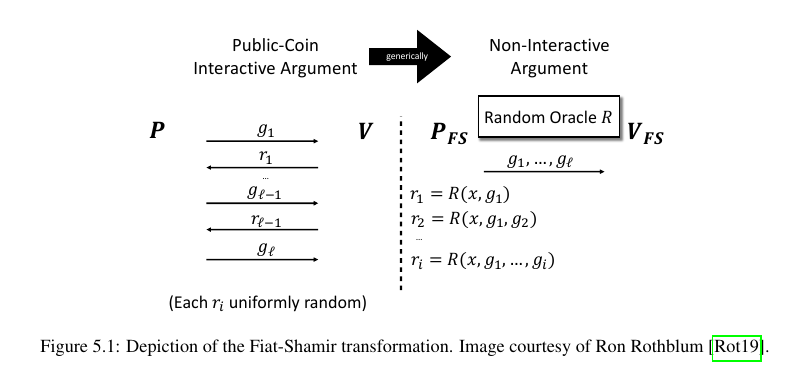
\includegraphics[scale=0.5]{fiat-shamir}
\end{figure}

\begin{boxx1}[the Fiat-Shamir transformation] \label{def:fiat-shamir}
Given an interactive protocol $\mathcal{I}$, the associated non-interactive protocol $\mathcal{Q}$ derived from the random oracle $R$ is defined as follows: the verifier $\mathcal{V}$'s message in round $i$ of $\mathcal{I}$ is determined by querying the random oracle with the input as the list of messages $g_1, \dots, g_i$ sent by the prover $\mathcal{P}$ in rounds $1, \dots, i$. As such, the prover $\mathcal{P}$ can simply send a single message containing the transcript of the entire protocol.
\end{boxx1}

\textbf{A Common Vulnerability}. As noted in the above definition, $r_i$ in $\mathcal{Q}$ is determined by the hash of the list of $g_1, \dots, g_i$. However, when an adversary can choose the input $x$ to the IP, it is essential to include $x$ into the list that is hashed in each round (as showed in the above figure). In fact, take the GKR protocol as an example, suppose the adversary can choose $x$ and it is known that the $\mathcal{V}$'s evaluation $\widetilde{x}(r) = c$ where $x$ is the input, $r$ is chosen randomly and $c$ is derived from previous rounds. Although this verification happens at the end of the protocol, one should include $x$ in each round's input: $R(x, g_1, \dots, g_i)$. Otherwise, the adversary can choose any $x \in \F^n$ such that $\widetilde{x}(r) = c$.

\textbf{Completeness and Soundness}. The completeness of the Fiat-Shamir transformation is clear: the non-interactive protocol $\mathcal{Q}$ is complete assuming the initial interactive protocol $\mathcal{I}$ is.

Suppose $y$ is not the right output of the input $x$. It has been known that when the Fiat-Shamir transformation is applied to a \textit{constant-round} IP $\mathcal{I}$ with negligible soundness error, the resulting non-interactive proof $\mathcal{Q}$ in the random oracle is sound against cheating provers that run n polynomial time. To illustrate the main idea, we use $3$-message protocol (e.g.,  $\Sigma$-protocol) as an example. 


\begin{boxx3}[Soundness in the ROM for $3$-message protocol]
Let $\mathcal{I}$ be a $3$-message protocol (e.g., $\Sigma$-protocols) with negligible soundness error, and let $\mathcal{Q}$ be the non-interactive protocol in the random oracle model obtained by applying the Fiat-Shamir transformation to $\mathcal{I}$. Then $\mathcal{Q}$ has negligible computational soundness error. That is, no polynomial prover can convince the verifier in $\mathcal{Q}$ of a false statement with non-negligible probability.
\end{boxx3}


\begin{figure}[H]
\centering
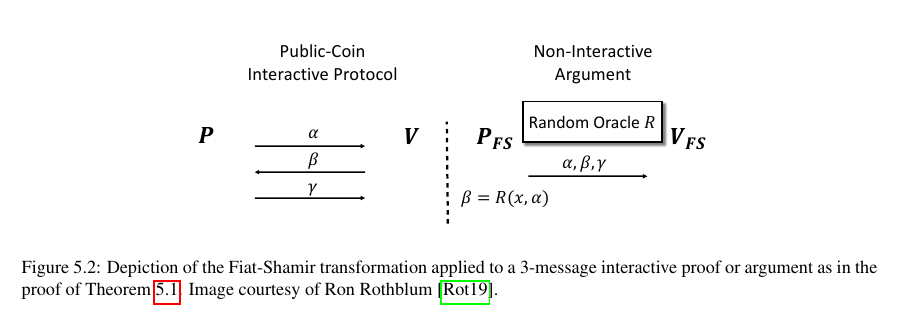
\includegraphics[scale=0.5]{sigma-fiat-shamir}
\end{figure}

Let $\mathcal{P_{FS}}$ is a prover in $\mathcal{Q}$ that runs in time $T$ and convinces the verifier to accept on input $x$ with probability at least $\epsilon$ (even in a cheating way). We will show that there is a prover $\mathcal{P}^{\displaystyle *}$ for $\mathcal{I}$ that convinces the verifier in $\mathcal{I}$ to accept with probability at least $\epsilon^{\displaystyle *} \geq \Omega(\epsilon/T)$ which contradicts the soundness of $\mathcal{I}$ by assumption. 

The simplest case is that, in order to get the accepting transcript $(\alpha, \beta, \gamma)$, $\mathcal{P_{FS}}$ has done in the (honest) way as showed in the above figure. Note that here $\mathcal{P_{FS}}$ only accomplish \textit{only one} query with the input $(x, \alpha)$ where $x$ is the input of the protocol (as $h = g^{w}$ in the $\Sigma$-protocol) and $\alpha$ is chosen uniformly at random by $\mathcal{P_{FS}}$. In this case, the prover $\mathcal{P}^{\displaystyle *}$ in the interactive protocol $\mathcal{I}$ can be designed to run $\mathcal{P_{FS}}$ in the first step to get a random $\alpha$, after the verifier $\mathcal{V}$ reply with a challenge $\beta$ (as $\mathcal{I}$ is interactive), $\mathcal{P_{FS}}$ then uses $\beta$ as the response of the random oracle $R(x, \alpha)$ to $\mathcal{P_{FS}}$, since it seems indistinguishable from $\mathcal{P_{FS}}$ based on assumptions of ROM. $\mathcal{P}^{\displaystyle *}$ continues running $\mathcal{P_{FS}}$ until $\mathcal{P_{FS}}$ terminates. This ensures that $\mathcal{P}^{\displaystyle *}$ convinces the verifier in $\mathcal{I}$ to accept $(\alpha, \beta, \gamma)$ with the same probability as $\mathcal{P_{FS}}$ does. 

In the general case, $\mathcal{P_{FS}}$ may ask the random oracle \textit{many} queries, say $T$ queries. This means, $\mathcal{P}^{\displaystyle *}$ may not have a clue about at which point $(x, \alpha)$ $\mathcal{P_{FS}}$ has used to get the accepting transcript $(\alpha, \beta, \gamma)$, if we follow the same strategy as above. To make the assumption more clear, we may suppose $\mathcal{P_{FS}}$ exactly makes $T$ \textit{distinct} queries $(x, \alpha_i)$ to $R$, and $(x, \alpha)$ is one of them where $\alpha$ corresponds to the final accepting transcript $(\alpha, \beta, \gamma)$.

Under these assumptions, we design $\mathcal{P}^{\displaystyle *}$ to simply pick a random integer $i \in \left\{ 1, \dots, T \right\}$ first, then runs $\mathcal{P_{FS}}$ up until its $i$-th query. Note the probability of $\mathcal{P_{FS}}$ making its $i$-th query as $(x, \alpha)$ is $1/T$. Then $\mathcal{P}^{\displaystyle *}$ sends $\alpha$ to the verifier $\mathcal{V}$ in $\mathcal{I}$, and take the response challenge $\beta$ from $\mathcal{V}$ to serve as the random oracle's response $\beta = R(x, \alpha)$ to $\mathcal{P_{FS}}$. Note that to ensure the integrity of the running of $\mathcal{P_{FS}}$, $\mathcal{P}^{\displaystyle *}$ should run $\mathcal{P_{FS}}$ for the remaining $T-i$ queries. Finally, $\mathcal{P}^{\displaystyle *}$ get the same accepting transcript $(\alpha, \beta, \gamma)$ if $\mathcal{P_{FS}}$ does. 

\begin{remark}
Based on the assumptions about ROM, the prover $\mathcal{P_{FS}}$ has no knowledge of what the value $R(a, \alpha)$ would be like. Thus, $\mathcal{P}^{\displaystyle *}$ could feed any random-like value to $\mathcal{P_{FS}}$ as $R(x, \alpha)$ which is important for the rewinding process. 
\end{remark}

\subsection{Fiat-Shamir Applied to $\Sigma$-Protocol and Forking Lemmas}\label{sec:fiat-shamir-forking-lemmas}

In this section, we explain that applying the Fiat-Shamir transformation to any $\Sigma$-protocol (such as Schnorr's). We follow the same notations as in the first two sections. We will mainly focus on the property of \textit{special soundness} of the Fiat-Shamir-ed version $\mathcal{Q}$ derived from the interactive Schnorr's protocol $\mathcal{I}$. 

Suppose $\mathcal{P_{FS}}$ produces an accepting transcript on input $h$ with probability $\geq \epsilon$. We next prove that, by running twice, $\mathcal{P_{FS}}$ is capable of getting two accepting transcripts $(a, e, z)$ and $(a, e', z')$ with $e \neq e'$, with probability $\geq \Omega(\epsilon^4 / T^3)$ where $T$ is the runtime of $\mathcal{P_{FS}}$.

The idea here is to fix the value of any internal randomness used by $\mathcal{P_{FS}}$ first, after running once $\mathcal{P_{FS}}$ to get an accepting transcript $(a, e, z)$ where $e = R(h, a)$, with probability $\geq \epsilon$, \textit{rewind} $\mathcal{P_{FS}}$ to just before it queries $R$ at $(h, a)$ and change $R$'s response \textit{artificially} (as explained at the end of last section) from $e$ to a fresh randomly chosen $e'$. Then run $\mathcal{P_{FS}}$ once again to completion to get another accepting transcript $(a, e', z')$. Since $e' = e$ is only with probability $1/2^{\lambda}$ where $\lambda$ denotes the length of bits output by $R$, we may assume $e \neq e'$ which will affect the success probability at most $1/2^{\lambda}$. 

\textbf{Forking lemmas}. The result is derived from so-called \textit{forking lemmas}. Assuming $\mathcal{P_{FS}}$ makes its $i^{\displaystyle *}$-th query at $(h, a)$ for the accepting transcript $(a, e, z)$. Forking lemmas express the fact that during the $T$ queries made by $\mathcal{P_{FS}}$, the witness extraction procedure runs $\mathcal{P_{FS}}$ twice, once using responses $(X, Y)$ and once using $(X, Y')$, where $X$ denote captures the random oracle's first $i^{\displaystyle *} - 1$ queries, and $Y$ and $Y'$ capture the remaining $T - i^{\displaystyle *} + 1$ queries. Note that in this way, the first $i^{\displaystyle *}$ query points are fixed the same for both runnings, especially the $i^{\displaystyle *}$-th query is at $(h, a)$. One thinks of the random oracle generation process as "forking" into two different paths after the first $i^{\displaystyle *}$ queries are finished. 

The forking lemma is based on the following result from probability theory.

\begin{boxx2}
Suppose $(X, Y)$ are jointly distributed random variables and let $A(X, Y)$ be any event such that $\Prr[A(X, Y)] \geq \epsilon$. Let $\mu_X$ be the marginal distribution of $X$, and for $x$ in the support of $\mu_X$, call $x$ good if the conditional probability $\Prr[A(X, Y) \vert X = x] \geq \epsilon/2$. Let $p = \Prr_{x \leftarrow \mu_X} [x \text{ is good }]$. Then $p \geq \epsilon/2$. \end{boxx2}

\begin{proof}
See Claim 12.1 \cite{ThalerBookZKP}.
\end{proof}

\textbf{Remarks}.
\begin{itemize}
\item Note that there are \textit{two parts of randomness} regarding the prover $\mathcal{P_{FS}}$. One part is from the \textit{internal randomness} in $\mathcal{P_{FS}}$ which involves picking values of $a$ and $z$ for example; the other part is simply the randomness of evaluating the random oracle $R$. 

Let $X$ equal to $\mathcal{P_{FS}}$'s internal randomness, $Y$ equal to the randomness of evaluating the random oracle $R$, and the event $A$ equal to $\mathcal{P_{FS}}$ gets the accepting transcript $(a, e, z)$ with the internal randomness $X$ and random oracle $Y$. The proposition tells that the internal randomness is "good" with probability $\geq \epsilon/2$, where being good, by definition, means $\Prr[A(X, Y) \vert X = x] \geq \epsilon/2$. 

Fix the random variable $X$ with such "good" assignments, we next consider the conditional probability
\begin{equation*}
\Prr \left[  (\mathcal{P_{FS}} \text{ wins}) \vert X \text{ is good}\right] \geq \epsilon/2
\end{equation*}
which gets rid of the internal randomness of $\mathcal{P_{FS}}$, we may hence consider $\mathcal{P_{FS}}$ as a \textit{deterministic} algorithm that wins with probability at least $\epsilon/2$ over the random choice of query responses from $R$. We will omit the conditional part and denote only the event in $ (\mathcal{P_{FS}} \text{ wins})$.
\item Let $Q_1, \dots, Q_T$ denotes the random variables about $\mathcal{P_{FS}}$'s $T$ query points to $R$, which can fully express the event. We may easily prove that there is at least one integer $i^{\displaystyle *} \in \left\{ 1, \cdot, T \right\}$ such that (see Claim 12.2.3 \cite{ThalerBookZKP}, remember that $\mathop{\Prr}_R \left[ \mathcal{P_{FS}} \text{ wins} \right] \geq \epsilon/2$ assuming $X$ is good and at least one query at $(h, a)$ given the accepting transcript is $(a, e, z)$).
\begin{equation*}
\mathop{\Prr}_R \left[ (\mathcal{P_{FS}} \text{ wins}) \cap Q_{i^{\displaystyle *}} = (h, a) \right] \geq \epsilon/(2T)
\end{equation*}
Fix such $i^{\displaystyle *}$, apply the above proposition again to the event $A$ as $(\mathcal{P_{FS}} \text{ wins}) \cap Q_{i^{\displaystyle *}} = (h, a)$ with the random variable $X$ as the first $i^{\displaystyle *} - 1$ query points, and $Y$ as the remaining $T - i^{\displaystyle *} + 1$ query points. We may define as well $X = x$ is "good" accordingly. More precisely, $x$ are the $i^{\displaystyle *} - 1$ query points of $\mathcal{P_{FS}}$ such that $\mathcal{P_{FS}}$ wins and the $i^{\displaystyle *}$-th query point is $(h, a)$. Therefore, by the proposition the probability of $X$ is good, i.e., the $i^{\displaystyle *} - 1$ query points taking such values, is at least $\epsilon/4T$. Besides, by definition for such $X = x$, the probability that $\mathcal{P_{FS}}$ wins while $Q_{i^{\displaystyle *}} = (h, a)$ is at least $\epsilon/(4T)$. 
\item Finally, to obtain two accepting transcripts $(a, e, z)$ and $(a, e', z')$, we first focus on the event $X = x$ is good as defined above, that means the assignments for the first $i^{\displaystyle *} - 1$ query points are good and the $i^{\displaystyle *}$-th query point is $(h, a)$ such that $\mathcal{P_{FS}} \text{ wins}$, the probability is at least $\epsilon/(4T)$. Then we draw \textit{two independent} copies $Y$ and $Y'$. The event that $\mathcal{P_{FS}}$ gets the required two transcripts equals to the event that $Y$ and $Y'$ satisfy the event $A$ defined above, thus the probability is
\begin{equation*}
\mathop{\Prr}_{x \leftarrow X} \left[ x \text{ is good} \right] \cdot \mathop{\Prr}_Y \left[ A(x, Y) \vert x \text{ is good} \right] \cdot \mathop{\Prr}_Y \left[ A(x, Y') \vert x \text{ is good} \right] \geq (\epsilon/(4T))^3
\end{equation*}
Plus the precedent factor $\epsilon/2$ about the internal randomness, the result follows. 
\end{itemize}

\subsection{A Homomorphic Commitment Scheme Derived From the $\Sigma$-Protocols}

\textbf{Commitment Schemes}. In a commitment scheme, there are two parties, a committer and a verifier. We may think of the scheme as the scenario of first sealing and later opening an envelope. The two parties first agree on a key generation procedure, then two phases will be processed in the scheme: 
\begin{itemize}
\item \textsf{KeyGen} is a random algorithm that generates a commitment key \textsf{ck} known to the committer and a verification key \textsf{vk} known to the verifier. The two keys can be identical.
\item The \textit{commit phase}. The committer runs a random algorithm \textsf{Commit} that takes as input the commitment key \textsf{ck} and the message $m$ to be committed. It outputs the commitment $c$, as well as extra opening information $d$. Such opening information will be only revealed to the verifier during the verification phase. The committer should be unable to open to the commitment to any value other than $m$. The property is called \textit{binding}. 
\begin{equation*}
\text{\textsf{Commit}}(\text{\textsf{ck}}, m) = (c, d)
\end{equation*}
\item The \textit{verification phase}. The verifier runs a random algorithm \textsf{Verify} that takes with input the verification key \textsf{vk}, the commitment $c$ as well as the extra opening information $d$, and a claimed message $m'$. The output is \textsf{Accept} or not. But no extra information about the message $m$ should be revealed. The property is called \textit{hiding}. 
\begin{equation*}
\text{\textsf{Verify}}(\text{\textsf{vk}}, (c, d), m') = 1 \text{ or } 0
\end{equation*}
\end{itemize} 

\textbf{A Perfectly Hiding and Computationally binding Commitment Scheme from any $\Sigma$-Protocol}. Recall a relation $\mathcal{R}$ specifies a collection of valid instance-witness pairs $(h, w)$. For example, given a group $\mathbb{G}$ and a generator $g$, the discrete logarithm relation $\mathcal{R}_{DL}(\mathbb{G}, g)$ is the collection of pairs $(h, w) \in \mathbb{G} \times \Z$ such that $h = g^w$. We will demonstrate how to use any $\Sigma$-protocol for any hard relation $\mathcal{R}$ to obtain a \textit{perfectly hiding, computationally binding} commitment scheme. \label{sec:pedersen-commitment}

Recall the simulator used in Schnorr's protocol with input $h$, first picks uniformly at random the challenge $e \in \left\{ 0, \dots, \abs{\mathbb{G}} - 1 \right\}$, then picks uniformly at random $z \in \left\{ 0, \dots, \abs{\mathbb{G}} - 1 \right\}$ as well. Hence, 
\begin{equation*}
a = g^z \cdot h^{-e}
\end{equation*}
and the transcript $(a, e, z)$ follows the same distribution as in the $\Sigma$-protocol. Note that in the initial protocol, the first message $a$ is independent of the verifier's message $e$, thus in the transcript generated by the simulator the fact is still true as they follow the same distribution. 

Now, make the simulator not only takes the input of $h$, but also a \textit{fixed} challenge $e^{\displaystyle *}$. After taking $z$ uniformly at random, the output is still an accepting transcript $(a, e^{\displaystyle *}, z)$. Here $e^{\displaystyle *}$ is also independent of $a$ by the above remark. 

Here is how Dam\aa rd's commitment scheme works for any $\Sigma$-protocol: 
\begin{enumerate}
\item\label{item:35} Based on the hard relation $\mathcal{R}$, get a instance-witness pair
\begin{equation*}
(h, w) \leftarrow \text{\textsf{Gen}}
\end{equation*}
And make the commitment key and verification key as $\text{\textsf{ck}} = \text{\textsf{vk}} = h$. Note that the witness $w$ is "toxic waste" which should be discarded, as it will lead to break binding ($a$ is the commitment to $e = m$). 
\item\label{item:36} For the commitment phase, the committer runs the simulator with input $h$ and $e^{\displaystyle *} = m$, the output is the transcript $(a, e^{\displaystyle *}, z)$. Then the committer sends $a$ as the commitment, and keeps $e^{\displaystyle *} = m$ and $z$ as opening information. 
\item\label{item:37} In the verification phase, the committer first sends the opening information $e^{\displaystyle *} = m$ and $z$ to the verifier. Then the verifier checks $(a, e^{\displaystyle *}, z)$ is an accepting transcript for the public input $h$. 
\end{enumerate}

For the commitment scheme, we should analyze correctness, computational binding and perfect hiding. 
\begin{itemize}
\item \textbf{Correctness} is immediate as the HVZK property of the $\Sigma$-protocol guarantees that the simulator only outputs accepting transcripts for honest prover.  
\item \textbf{Perfect hiding} follows from the above remark that, the commitment $a$ is independent of the message $e^{\displaystyle *} = m$. 
\item \textbf{Computational binding} follows from special soundness of the $\Sigma$-protocol. Think about for the same commitment $a$ and two sets of opening information: $(e, z)$ and $(e', z')$ that both cause the verifier to accept, then $(a, e, z)$ and $(a, e', z')$ must be accepting transcripts. By definition of the $\Sigma$-protocol, the witness can be recovered such that $(h, w) \in \mathcal{R}$, which contradicts $\mathcal{R}$ is computationally hard. 
\end{itemize}

\subsection{Pedersen Commitments}

By instantiating Dam\aa rd's construction with Schnorr's protocol, one recovers a well-known commitment scheme due to Pedersen. 

Note here the presentation of the protocol is slightly different from the one given in the last section. The commitment $a$ is computed by
\begin{equation*}
c = g^m \cdot h^z
\end{equation*}
Note that the corresponding accepting transcript in Schnorr's protocol becomes
\begin{equation*}
\begin{cases}
(c, -z, m)   &\text{ in Pedersen commitments} \\
 (a, e,  z)  &\text{ in Schnorr's protocol}
\end{cases}
\end{equation*}

Also, the random group element $h^z$ acts as a "blinding factor" so that the product $a$ is independent of the message $m$.

Another notable fact is that the key generation procedure is capable of generating a random \textit{group element} $h$ directly, without producing the "toxic waste" $w$ with $g^w = h$. 

\begin{boxx1}[Pedersen Commitments] \label{def:pedersen-commitments}
Let $\mathbb{G}$ be a multiplicative cyclic group of prime order. 
\begin{enumerate}
\item\label{item:39} The key generation procedure publishes randomly chosen generator $g \in \mathbb{G}$ and a random group element $h \in \mathbb{G}$. Let $\text{\textsf{ck}} = \text{\textsf{vk}} = (g, h)$. 
\item\label{item:40} To commit to a message $m \in \left\{ 0, \dots, \abs{\mathbb{G}} - 1 \right\}$, the committer picks a random $z \in \left\{ 0, \dots, \abs{\mathbb{G}} - 1 \right\}$ and sends $c = g^m \cdot h^z$ to the verifier. 
\item\label{item:41} To open the commitment by the verifier, the committer sends the opening information $(m, z)$ to the verifier and it will check that $c = g^m \cdot h^z$, i.e., $(c, -z, m)$ is an accepting transcript of Schnorr's protocol. 
\end{enumerate}
\end{boxx1}

Next, we will study several important properties of Pedersen commitments.

\textbf{Additive Homomorphism}. It means given two commitments $c_1$ and $c_2$ associated with $m_1$ and $m_2$, respectively, then the verifier can derive on its own a commitment $c_3 = c_1 \cdot c_2$ to the new message $m_3 = m_1 + m_2$. This can be seen as
\begin{equation*}
g^{m_1 + m_2} \cdot h^{z_{1} + z_{2}}  = c_1 \cdot c_2 = c_3
\end{equation*}

\textbf{Perfect HVZK Proof of Knowledge of Opening}. We introduce here a perfect HVZK proof for the knowledge of opening Pedersen commitments. The idea is basically based on the additive homomorphism of Pedersen commitments and Schnorr's protocol.

For the prover $\mathcal{P}$ to prove it knows the opening information $m, z$ such that the commit $c$ satisfies $c = g^m \cdot h^z$. The proof is processed as follows: 
\begin{boxx1}[Zero-Knowledge Proof of Knowledge of Opening of Pedersen Commitment] \label{def:zk-opening-pedersen}
Let $\mathbb{G}$ be a multiplicative cyclic group of prime order, the generator $g$ and a group element $h$ are chosen randomly and known to all. Let $c$ public to both $\mathcal{P}$ and $\mathcal{V}$. $\mathcal{P}$ aims to prove the witness $(m, z)$ (as opening information) of $c$ where $c = g^m \cdot h^z$.
\begin{enumerate}
\item\label{item:42} $\mathcal{P}$ sends a group element $c' = g^{m'} \cdot h^{z'}$ for a random pair $(m', z')$ (the pair is secret to the verifier). One could think of $c'$ as a commitment to $m'$ using randomness $z'$. 
\item\label{item:43} The verifier $\mathcal{V}$ sends a random challenge $e$ to $\mathcal{P}$, also $\mathcal{V}$ can derive a commitment $c^{\displaystyle *} = c^e \cdot c' = g^{me + m'} \cdot h^{ze + z'}$ to the message $me + m'$ using randomness $ze + z'$, by additive homomorphism. Note that only $c^e$ and $c'$ are known to $\mathcal{V}$.
\item\label{item:44} Then $\mathcal{P}$ responds with opening information $(\alpha, \beta) = (me + m', ze + z')$, so that $\mathcal{V}$ can check $c^{\displaystyle *} = g^{me + m'} \cdot h^{ze + z'}$.
\end{enumerate}
In summary, an accepting transcript of three messages in this protocol is in the form of $(c', e, (\alpha, \beta))$ such that $c^{\displaystyle *} = c^e \cdot c' = g^{\alpha} \cdot h^{\beta}$.
\end{boxx1}

\begin{remark}
This proof is very similar to Schnorr's protocol. In order to prove the knowledge of $(m, z)$ with $g^m \cdot h^z = c$,
\begin{itemize}
\item the prover first chooses another random pair $(m', z')$, then the final pair $(me + m', ze + z')$ is \textit{statistically independent} of the opening information $(m, z)$ of $c$ 
\item the challenge $e$ given by $\mathcal{V}$ is used to ensure \textit{special soundness} as showed below ($m$ can be extracted)
\item the prover finally sends $(\alpha, \beta) = (me + m', ze + z')$ so that $\mathcal{V}$ can check $g^{\alpha} \cdot h^{\beta} = c^e \cdot c'$ for $c = g^m \cdot h^z$ and $c' = g^{m'} \cdot h^{z'}$, both are known to the verifier. Therefore, the witness here is a vector $(m, z)$ instead of a simple $w$ in the initial Schnorr's protocol, while the completeness and special soundness are exactly the same as in Schnorr's protocol. 
\end{itemize}
\end{remark}

As a zk-proof, the following three properties are essential to analyze:
\begin{itemize}
\item Perfect completeness. If $\mathcal{P}$ follows the above prescribed protocol, the result should be accept. 
\item Special soundness. Exactly as in Schnorr's protocol, we use two accepting transcripts of the $\Sigma$-protocol:
\begin{align*}
& (c', e, (me + m', ze + z')) \\
& (c', e^{\displaystyle *}, (me^{\displaystyle *} + m', ze^{\displaystyle *} + z'))
\end{align*}
Note that $m'$ and $z'$ are fixed as $c'$ remains the same in the first round for the two transcripts. The challenges $e$ and $e^{\displaystyle *}$ are different. The goal is to recover $(m, z)$ and prove it is the \textit{opening information} of the initial commitment $c$. Denote 
\begin{equation*}
\begin{split}
(me + m', ze + z') &= (\alpha_1, \beta_1) \\
(me^{\displaystyle *} + m', ze^{\displaystyle *} + z') &= (\alpha_2, \beta_2)
\end{split}
\end{equation*}
where $\alpha_i, \beta_i$ are sent to $\mathcal{V}$ from $\mathcal{P}$. The extractor is to recover $(m, z)$ as follows
\begin{equation*}
\alpha_1 - \alpha_2 = m (e - e^{\displaystyle *}) \Rightarrow m = (\alpha_1 - \alpha_2)(e - e^{\displaystyle *})^{-1} \mod \abs{\mathbb{G}}
\end{equation*}
The same method applies to recovering $z$ while using $\beta_1, \beta_2$. Finally, we should prove that $(m, z)$ is the opening information of $c$. As
\begin{equation*}
\begin{cases}
c^{e} \cdot c' = g^{\alpha_1} \cdot h^{\beta_1} \\
c^{e^{\displaystyle *}} \cdot c' = g^{\alpha_{2}} \cdot h^{\beta_{2}} \\
\end{cases}
\end{equation*}
dividing the first equation by the second one and power with $(e - e^{\displaystyle *})^{-1}$, we get
\begin{equation*}
c = g^{(\alpha_1 - \alpha_2) (e - e^{\displaystyle *})^{-1}} \cdot h^{(\beta_1 - \beta_2)(e - e^{\displaystyle *})^{-1}} = g^{m} \cdot h^z 
\end{equation*}
where the result follows.

\item Perfect HVZK. Recall the transcript is $(c', e, (\alpha, \beta))$ where two of the three parts are uniform at random. Then a simulator can generate transcripts in the same distribution via: 

\begin{enumerate}
\item\label{item:38} Pick uniformly at random $e \in \left\{ 0, \dots, \abs{\mathbb{G}} - 1 \right\}$. 
\item\label{item:45} Pick uniformly at random the pair $(\alpha, \beta) \in \left\{ 0, \dots, \abs{\mathbb{G}} - 1 \right\}^2$. 
\item\label{item:46} Set $c' = g^{\alpha} \cdot h^{\beta} \cdot c^{-e} = c^{\displaystyle *} \cdot c^{-e}$.
\end{enumerate}
\end{itemize}

\textbf{A Product Relationship Between Committed Values}. Let's fix some notations first. The Pedersen commitment picks public two generators $g, h \in \mathbb{G}$ first. To commit a message $m \in \left\{ 0, 1, \dots, \abs{\mathbb{G}} - 1 \right\}$, the protocol takes the commitment as $c = g^m \cdot h^z \in \mathbb{G}$ where some blinding factor is chosen as $z \in \left\{ 0, \dots, \abs{\mathbb{G}} \right\}$. We may simple denote the relations as
\begin{equation*}
c = \text{Com}_{g, h}(m, z)
\end{equation*}
We have already seen the Pedersen commitments are additively homomorphic, meaning given $c_{1} = \text{Com}_{g, h}(m_{1}, r_1)$ and $c_{2} = \text{Com}_{g, h}(m_{2}, r_2)$, the verifier can derive \textit{on its own}
\begin{equation*}
c_1 \cdot c_2 = \text{Com}_{g, h}(m_1 + m_2, r_1 + r_2)
\end{equation*}
The question is, given the information as above in the additive case,  how the prover $\mathcal{P}$ can prove to the verifier $\mathcal{V}$ that $c_3$ is the commitment to the message $m_1 \cdot m_2$ without actually revealing $m_1 \cdot m_2$? The key remark is the following equivalence:
\begin{equation*}
\begin{split}
c_{3} & = \text{Com}_{g, h}(m_1 \cdot m_2, r_3) \\
c_3 & = \text{Com}_{c_1, h}(m_2, r_3 - r_1m_2) \quad \text{ for } c_1 = g^{m_1} h^{r_1}
\end{split}
\end{equation*}
Therefore, the product relation $m_1 \cdot m_2$ is transferred into a single message $m_2$ in cost of changing the generator. Thus, we can use the \textit{latter representation} for the product relation. 

Given $c_i = \text{Com}_{g, h}(m_i, r_i), i = 1, 2, 3$ where $m_3 = m_1 \cdot m_2$, to get zk-proof of $(m_3, r_3)$, similar to the last protocol the prover chooses two independent commitments to $c_1$ and $c_2$ by
\begin{equation*}
\begin{split}
\alpha & = \text{Com}_{g, h}(b_1, b_2) \\
\beta & = \text{Com}_{g, h}(b_3, b_4)
\end{split}
\end{equation*}
Using the alternative expression of $c_3$, the prover constructs the corresponding commitment
\begin{equation*}
\gamma = \text{Com}_{c_1, h}(b_3, b_5)
\end{equation*}
Hence, the prover sends $\alpha, \beta$ and $\gamma$ to the verifier in the first round. By applying a challenge $e$, the verifier can derive \textit{on its own} the following commitments using additive homomorphism:
\begin{equation*}
\begin{split}
\alpha \cdot c_1^e & = \text{Com}_{g, h}(b_1 + e \cdot m_1 , b_2 + e \cdot r_1) \\
\beta \cdot c_{2}^e & = \text{Com}_{g, h}(b_{3} + e \cdot m_2 , b_4 + e \cdot r_2) \\
\gamma \cdot c_3^e & = \text{Com}_{c_1, h}(b_{3} + e \cdot m_{2} , b_{5} + e \cdot (r_3 - r_1 m_2))
\end{split}
\end{equation*}
The opening of the three commitments $(b_1 + e c\dot m_1, b_2 + e \cdot r_1), \dots $ will be provided by the prover in the final round. Thus, the verifier can check the validity of $c_3$ to $m_1 \cdot m_2$ in the three relations. Formal details are given below

\begin{boxx1}[ZK of Opening of Pedersen Commitments Satisfying Product Relationship] \label{def:zk-product-pedersen}
Let $\mathbb{G}$ be a multiplicative cyclic group of prime order over which the Discrete Logarithm relation is hard. 
\begin{enumerate}
\item\label{item:59} Input is $c_i = g^{m_i} \cdot h^{r_i} c = \text{Com}_{g, h}(m_i, r_i)$ for $i \in \left\{ 1, 2, 3 \right\}$ such that $m_3 = m_1 \cdot m_2 \mod \abs{\mathbb{G}}$. 
\item\label{item:60} The prover knows $c_i, m_i, r_i$ for all $i$, and the verifier knows $c_1, c_2, c_3, g, h$. 
\item\label{item:61} The prover picks randomly $b_1, \dots, b_5 \in \left\{ 0, \dots, \abs{\mathbb{G}} - 1 \right\}$ and sends to the verifier with the three values $\alpha, \beta$ and $\gamma$ satisfying 
\begin{equation*}
\alpha = g^{b_1} \cdot h^{b_2};  \quad \beta = g^{b_3} \cdot h^{b_4};  \quad \gamma = c_1^{b_3} \cdot h^{b_5}
\end{equation*}
\item\label{item:62} The verifier sends to the verifier with a challenge $e$ chosen at random in $\left\{ 0, \dots, \abs{\mathbb{G}}-1 \right\}$. 
\item\label{item:63} The prover sends to the verifier with the values $z_1, z_2, z_3, z_4$ and $z_5$ satisfying 
\begin{equation*}
z_1 = b_1 + e \cdot m_1; \quad z_2 = b_2 + e \cdot r_1; \quad z_3 = b_3 + e \cdot m_2; \quad z_4 = b_4 + e \cdot r_2 ; \quad z_5 = b_5 + e \cdot (r_3 - r_1 m_2)
\end{equation*}
\item\label{item:64} The verifier checks the following equality
\begin{equation*}
g^{z_1} \cdot h^{z_2} = \alpha \cdot c_1^e; \quad g^{z_3} \cdot h^{z_4} = \beta \cdot c_2^e; \quad c_1^{z_3} \cdot h^{z_5} = \gamma \cdot c_3^e
\end{equation*}
\end{enumerate}
\end{boxx1}

\textbf{Completeness, special soundness, and honest-verifier zero-knowledge}. Since this is a zk-proof (about the opening for the commitment $c_3$), the three properties are essential to analyze. The completeness is straightforward. Now we study the special soundness, that means an extractor $\mathcal{E}$ can be constructed to extract $(m_3, r_3)$ for the commitment $c_3$ when two accepting transcripts are given: 
\begin{equation*}
\left( \left( \alpha, \beta, \gamma \right), e, (z_1, \dots, z_5) \right) ; \quad \left( \left( \alpha, \beta, \gamma \right), e', (z_1', \dots, z_5') \right)
\end{equation*}
Apparently, applying $z_1 - z_1'$ etc, we can easily get $(m_1, r_1)$ and $(m_2, r_2)$. Especially, 
\begin{equation*}
z_5 - z_5' = (e - e') \cdot (r_3 - r_1m_2)
\end{equation*}
gives the value of $r_3$. In all, the knowledge of opening of $c_3$ is given by $(m_1m_2, r_3)$.

\section{Zero-Knowledge via Commit-And-Prove and Masking Polynomials}

\subsection{Commit-and-Prove}

The zero-knowledge arguments introduced in the last chapter are based on Pedersen commitments. They provide the prover with the ability of proving its knowledge of opening some (public) commitment without revealing the committed values. In this part, we will study our first zero-knowledge arguments for circuit SAT using the precedent zk-proofs as subroutines. 

Given a circuit SAT instance $\mathcal{C}(x, w) = y$, the circuit $\mathcal{C}$, the input $x$ and the output $y$ are public to both $\mathcal{P}$ and $\mathcal{V}$, while the prover wants to establish that it knows the witness $w$ such that the relation holds, for simplicity we suppose $\mathcal{C}(w) = 1$. Recall we have learned two ways representing the circuit SAT: one is using the notion of \textit{correct transcript} which records values of each gate and the inputs, see Figure \ref{fig:circuit-transcript}; the other way is using the MLE of the functions representing values at each gate as treated in the GKR protocol, see Figure \ref{fig:circuit-MLE}. Both ways can be transferred into zero-knowledge arguments based on a technique called \textit{commit-and-prove}. 

Pedersen commitments satisfy the following properties: 
\begin{enumerate}[(a)]
\item\label{item:65} given $c_1$ and $c_2$, $c_1 \cdot c_2$ is \textit{automatically} the commitment of $m_1 + m_2$ \textit{without any further proof}
\item\label{item:66} given $c_1, c_2$ and $c_3$, there exists a zero-knowledge argument that the prover can prove to the verifier $c_3$ is the commitment of $m_1 \cdot m_2$. Note that the verifier \textit{can not} derive $c_3$ based on $c_1$ and $c_2$ \textit{on its own} without help from the prover. Hence, communication complexity should contain this point. 
\end{enumerate}
As addition and multiplication are a universal basis, meaning that with these two operations alone, one can compute \textit{arbitrary} functions of any input. Hence, a verifier is able to do arbitrary computation over committed values, without making the prover reveal the \textit{committed values}. 

\textbf{Commitment to Each Gate}. When applied to the first form of circuit SAT, the prover need to send the \textit{Pedersen commitments} to each \textit{multiplication} gate as well as each symbol of $w$, to the verifier, and prove in zero-knowledge that the \textit{committed values} satisfy the constraints of the gates in multiplication and addition. Note that the final step suffices to apply the Schnorr's protocol since the opening to the corresponding commitment is supposed to be $1$ thus public. 
\begin{enumerate}
\item\label{item:58} At the start of the protocol, the prover sends Pedersen commitments to each entry of $w$ as well as to the value of every multiplication gate in the circuit $\mathcal{C}$.  
\item\label{item:67} Then for each entry of witness $w$, the prover proves via Protocol \ref{def:zk-opening-pedersen} that the prover knows an opening of the commit to that entry. 
\item\label{item:68} Next, for each multiplication gate in the circuit, the prover uses Protocol \ref{def:zk-product-pedersen} to prove the committed value respects multiplication of the committed values of the two fan-in gates. As remarked earlier, addition gates are handled without any communication between prover and verifier. 
\item\label{item:69} Finally, at the end of the protocol, the prover uses Protocol \ref{def:schnorr} to prove knowledge of opening the commitment to the output gate $y = 1$, since the committed value is not secret.
\end{enumerate}

Therefore, the protocol is comprised of $\abs{w} + M + 1$ invocations of $\Sigma$-protocols where $M$ is the number of the multiplication gates. The three subroutines in Protocols \ref{def:schnorr}, \ref{def:zk-opening-pedersen} and \ref{def:zk-product-pedersen} make the resulting protocol \textit{complete and honest-verifier zero knowledge} (the simulator runs the simulator for each of these subroutines in sequence and concatenate the generated transcripts). A few more words about \textit{knowledge soundness}: given two accepting transcripts $(\mathbf{a}, \mathbf{e}, \mathbf{z})$ and $(\mathbf{a}, \mathbf{e'}, \mathbf{z'})$ where the bold letter stands for the transcripts of all gates. The extractor just runs the extractor for the corresponding subroutines while the addition gates can be ignored. Note that some gates values can be extracted multiple times. 

As to complexity analysis, the proof length is linear in the witness length and number of multiplication gates of $\mathcal{C}$. Moreover, the verifier's runtime  is linear in $\abs{\mathcal{C}}$ as the verifier should check every operation on the committed values. Next, we show how to reduce the proof length by combining commitment schemes with interactive proofs. 

\textbf{Combining with IPs}. Recall using IPs can reduce the proof length, for instance, the GKR protocol involves interactive actions between prover and verifier, also evaluations of MLE at random points in each layer render the protocol succinct as well. Note all such constructions don't take zero-knowledge into consideration. 

To render it zero-knowledge, the prover can send to the verifier with Pedersen commitments to each element of $w$. Also, recall the MLE involved in the GKR protocol \ref{def:GKR-protocol} and the low-degree univariate polynomials in the sum-check protocol \ref{def:sum-check-protocol} leak information about the witness $w$ to the verifier. To address this issue, the prover $\mathcal{P}$ sends Pedersen commitments to these coefficients (mainly for univariate polynomials in the most inner sum-check protocol) using Protocol \ref{def:zk-opening-pedersen} to show its knowledge of opening such commitments.

Now we may transfer the problem into the previous case using a new circuit $\mathcal{C}'$ and the corresponding input $w'$. The new circuit $\mathcal{C}'$ is based on the arithmetic gates involved in the computations about the GKR protocol (and of course the sum-check protocols as well). Hence, the input $w'$ should be the prover's messages (including the coefficients of polynomials) generated in the whole GKR protocol. Note the commitments mentioned above are exactly Pedersen commitments of $w'$, thus it remains to commit to the multiplication gates of $\mathcal{C}'$. The new communication complexity is thus $O(\abs{w} + d \log \abs{C})$ where $d$ is the depth of the initial circuit $\mathcal{C}$. In apparent ways, this protocol is complete, knowledge sound and honest-verifier zero-knowledge.

In summary, this sections gives a \textit{generic} way for transforming any IP into a zero-knowledge argument: \textit{the argument system prover} mimics the IP prover, but rather than sending the IP prover's message in the clear, it sends \textit{hiding commitments} to those messages, and proves in zero-knowledge that it knows how to open the commitments. At the end of the protocol, \textit{the argument verifier} mimics the IP verifier to check the validity, by exploiting homomorphism properties of the commitments. 

\subsection{Zero-Knowledge via Masking Polynomials}

In this section, we discuss another technique for transforming any IP into a zero-knowledge argument. Recall the core of the GKR protocol is to apply the sum-check protocol to $l$-variate polynomial, say $g(X)$ to check if it sums up to $G$. Suppose a \textit{polynomial commitment scheme} is available, meaning that the prover is able to cryptographically bind itself to the desired polynomial, say $p(X)$ (e.g. using $p(\tau)$ for some chosen $\tau$), then reveal the evaluation $p(r)$ for a random $r$ of the verifier's random choosing. 

We use the same notations as in Protocol \ref{def:sum-check-protocol}. To ensure the prover's messages in the sum-check protocol reveal no information about $g$, we mimic here the way in the $\Sigma$-protocol:

\begin{enumerate}
\item\label{item:70} the prover at the start of the protocol chooses a random polynomial $p$ with the same degree as $g$ in each variable. Note $p$ keeps secret to the verifier. Then it commits to $p$ using a polynomial commitment scheme, and send to the verifier a value $P$ claimed to equal
\begin{equation*}
P = \sum_{x \in \left\{ 0, 1 \right\}^l} p(x)
\end{equation*} 
\item\label{item:71} then the verifier picks a random $\rho \in \F \setminus \left\{ 0 \right\}$ as the challenge (like $e$ in the $\Sigma$-protocol) and send back to the prover 
\item\label{item:72} the two parties apply the sum-check protocol to the polynomial $g + \rho \cdot p$ and check 
\begin{equation} \label{eq:G+rho P}
G + \rho \cdot P = \sum_{x \in \left\{ 0, 1 \right\}^l} (g + \rho \cdot p)
\end{equation}
\item\label{item:73} at the end of the protocol, the verifier needs to evaluation the polynomial at a random input $r \in \F^l$:
\begin{equation*}
g(r) + \rho \cdot p(r)
\end{equation*}
where $g(r)$ can be obtained by the verifier with a single oracle query by assumption and $p(r)$ is got in the evaluation phase in the polynomial commitment scheme. 
\end{enumerate}

\textbf{Completeness and Soundness}. The protocol is clear complete. To see it is sound, suppose the value $G$ claimed by the prover is not equal to the sum $\sum g$, Equation (\ref{eq:G+rho P}) suggests that by solving an easy equation $a \cdot X + b = c$, there is only one choice for the random $\rho$, hence the soundness error probability is at most $1 / (\abs{\F} - 1)$.

\textbf{Honest-Verifier Zero-Knowledge}. By definition, the verifier should be able to construct a \textit{simulator} to simulate the transcripts \textit{on its own} while the transcript distribution remains the same as in the interactive proof. To this end, we should first figure out the generated transcript which is known to the verifier. Note that in this protocol, the value $G$ is fixed while the value $P, \rho$ and a random evaluation for the polynomial $(g + \rho \cdot p)(r)$ are known to $\mathcal{V}$ based on the sum-check protocol. Meanwhile, by assumption the verifier also has access to the evaluations $g(r)$ and $p(r)$ where $g$ is unknown to $\mathcal{V}$ and claimed to sum up to $G$, and $p(r)$ is revealed during the evaluation phase of the polynomial commitment.

The key point is, analogous to the $\Sigma$-protocol, to reorder the values. More precisely, 
\begin{enumerate}
\item\label{item:74} The simulator $\mathcal{S}$ selects a random polynomial $p$ subject to the degree bounds requirement. Then $\mathcal{S}$ commits to $p$ as usual and sets $P = \sum_{x \in \left\{ 0, 1 \right\}^l} p(x)$. 
\item\label{item:75} Then $\mathcal{S}$ picks at random the value $\rho \in \F \setminus \left\{ 0 \right\}$. 
\item\label{item:76} Next, choose a random query point $r \in \F^l$ and query $g(r)$ from the oracle. Then $\mathcal{V}$ chooses a random polynomial $f$ subject to 
\begin{equation*}
f(r) = g(r) \text{ and} \sum_{x \in \left\{ 0, 1 \right\}^l} f(x) = G = \sum_{x \in \left\{ 0, 1 \right\}^l} g(x)
\end{equation*}
\item\label{item:77} Finally, $\mathcal{S}$ computes the messages generated during the sum-check protocol applied to the polynomial $f + \rho \cdot p$. 
\end{enumerate}

\textbf{Masking $g(r)$}. Compared with the method of committing to circuit gates, using masking polynomials grants the verifier the access to evaluate $g(r)$ at the end of the sum-check protocol. However, this will violate zero-knowledge as $g$ itself depends on the witness $w$. We take for an instance with our 1st MIP in Section  \ref{sec:1st-MIP}.

This MIP is reduced to the sum-check protocol applied (only once) to the polynomial $h_{x, y, Z}(Y)$ where $x, y$ are fixed as input and output values, $Z: \F^k \rightarrow \F$ is a polynomial function involved in the expression which is \textit{not necessarily MLE}, and $Y$ takes values in $\F^{3k}$. Recall that an honest prover would take $Z$ as $\widetilde{W}$ of the correct transcript $W$ of the circuit, which would leak information of the witness $w$. 

Rather than taking directly $Z = \widetilde{W}$, the honest prover may the following \textit{random extension polynomial} of $W$:
\begin{equation*}
Z(X_1, \dots, X_{3k}) = \widetilde{W}(X_1, \dots, X_{3k}) + c_1X_1(1 - X_1) + c_2X_2(1 - X_2)
\end{equation*}
where $c_1$ and $c_2$ are chosen at random by the prover. 

\section{Polynomial Commitments from Hardness of Discrete Logarithm}

\subsection{A First Polynomial Commitment}

\textbf{A trivial polynomial commitment scheme}. An untrusted prover $\mathcal{P}$ has in its head a polynomial $q$ which is primarily a univariate or MLE polynomial. Suppose $\mathcal{P}$ sends a \textit{complete} description of $q$, say the list of all coefficients over an proper basis. Then the verifier $\mathcal{V}$, having learned $q$, can evaluate $q$ at any point $z$ of its choosing. This protocol is called the \textit{trivial polynomial commitment scheme}. 

The problems for the trivial polynomial commitment scheme are: 
\begin{itemize}
\item $q$ may be very large, in other words, it will be expensive to send a complete description of $q$ 
\item the verifier $\mathcal{V}$ learns the entire polynomial $q$, which may be incompatible with zero-knowledge (recall $q$ typically encodes a witness). 
\end{itemize}

\textbf{A zero-knowledge scheme with linear size commitments}. We begin by describing a scheme with linear size commitments thus it does not improve the costs of the trivial polynomial commitment scheme, but does render it zero-knowledge. In the remaining of this section, we keep the same idea and notions in Section \ref{sec:eval-polyn}.

Recall Pedersen commitments (see Definition \ref{def:pedersen-commitments}) are \textit{perfectly hiding and computationally binding} (see explanations in \ref{sec:pedersen-commitment}). Here we introduce a polynomial commitment scheme based on the Pedersen commitment: 

\textbf{Commitment Phase}. To commit to $q$, the prover sends a Pedersen commitment $c_i$ to each coefficient $u_i$ of the vector $u$, namely $c_i \leftarrow g^{u_i} \cdot h^{z_i}$. Since Pedersen commitments are hiding, so this reveals nothing to the verifier about the vector $u$. 

\textbf{Evaluation Phase}. Suppose the verifier evaluate at a random point $z$, let $y$ be the vector such that $q(z) = \langle u, y \rangle = \sum_i u_iy_i$. Since the verifier knows $y$ and all commitments $c_i$ to $u_i$, we view $c_i y_i$ as $y_i$ times of addition so that the verifier can derive \textit{on its own} a commitment $c$ to the quantity $\sum_i u_iy_i$. Finally, $\mathcal{P}$ can prove in zero-knowledge that it knows how to open the commitment $c$ via Protocol \ref{def:zk-opening-pedersen}. 

\textbf{Extractability}. When a polynomial commitment scheme is \textit{not} extractable, we mean the prover can prove it knows to open the commitment $c$ in the evaluation phase even though it is unable to open any of the commitment $c_i$ sent during the commitment phase. 

Let's see an example when the scheme is not extractable. Suppose the prover knows the evaluation point $z$ used by the verifier, \textit{prior to} sending the commitment $c_i$ to the polynomial to the verifier. For simplicity, assume the polynomial degree $n = 2$ and the blinding factor $h$ is identity, i.e the Pedersen commitment becomes $c_i = g^{m}$. 

Given the evaluation point $z$ and the prover intend to prove it can open the commitment $c$ to the evaluation value $a$ during the evaluation phase, it suffices to take an arbitrary $c_0 \in \mathbb{G}$ and $c_1 = (g^a \cdot c_0^{-1})^{z^{-1}}$. Therefore, the commitment during the evaluation phase is $c_0 \cdot c_1^z = g^a$ which is exactly the commitment to $u_0 + u_1z$. Note that here 
\begin{equation*}
u_1z \text{ is committed via } c_1^z \text{ by additive homomorphic property}
\end{equation*}
To address this issue, we may ask
\begin{enumerate}[(a)]
\item\label{item:82} during the commitment phase, not only the prover to make the commitments $c_i$ \textit{but also} to prove in zero-knowledge via Protocol \ref{def:zk-opening-pedersen} that it knows how to open $c_i$, then the extractable follows directly from the soundness of the protocol as all $u_i$ can be extracted from $c_i$; 
\item\label{item:83} as an alternative way, to make sure the random evaluation point $z$ is chosen by the verifier \textit{after} the prover has sent the commitments $c_i$ (without modifying the commitment phase as above). The extractability can be deduced as follows: given $n$ evaluation points $z^{(1)}, z^{(2)}, \dots, z^{(n)}$ and thus their evaluations $q(z^{(1)}), \dots, q(z^{(n)})$, the extractor $\mathcal{E}$ may get $n$ (very probably) independent \textit{linear} equations
\begin{equation*}
q(z^{(i)}) = \langle u, y^{(i)} \rangle = \sum_{j = 0}^{n-1} u_{j} y_{j} \quad \text{ for } y_j = (z^{(i)})^{j}
\end{equation*}
Hence, $\mathcal{E}$ can solve $u_i$ using Gaussian elimination. 
\end{enumerate}

\subsection{Pedersen Vector Commitments} \label{sec:peders-vect-comm}
The commitment introduced in the last section was as big as the polynomial being committed. We give a scheme that reduces the commitment size to constant in this section, which can be viewed as a \textit{compressing commitment}. 

\textbf{Commitment Phase}. To commit to a \textit{vector} $u \in \F^n$, choose at random $n$ generators $g_1, \dots, g_n \in \mathbb{G}$ and a random value $r_u \in \left\{ 0, 1, \dots, \abs{\mathbb{G}} - 1 \right\}$, send the following value to the verifier
\begin{equation*}
\text{Com} (u, r_u) = h^{r_u} \prod_{i = 1}^n g_i^{u_i}
\end{equation*}
This quantity is often referred to as \textit{Pedersen vector commitment}. Note that when $n = 1$ this commitment is merely the initial Pedersen commitment. Also, as the initial one the Pedersen commitment is additively homomorphic: given two vectors $u, v \in \F^n$ and any two \textit{scalars} $a_1, a_2 \in \F$, one can deduce the following relations
\begin{equation*}
\begin{split}
\text{Com}(a_1u, a_1r_1 ) & = \text{Com}^{a_1}(u, r_1 ) \\
\text{Com}(a_1u + a_2v, a_1r_1 + a_2r_2) & = \text{Com}^{a_1}(u, r_1 ) \cdot  \text{Com}^{a_2}(v, r_2 ) \\
c_{a_1u + a_2v} & = c_u^{a_1} \cdot c_v^{a_2}
\end{split}
\end{equation*}
\begin{itemize}
\item the last equality tells one can deduce \textit{on its own} the commitment to $a_1u + a_2v$ given the values of $a_1, a_2, c_u$ and $c_v$; 
\item we extend the additive homomorphism to scalar case
\end{itemize}

\textbf{Evaluation Phase}. The prover should prove that it knows how to open the commitment to the value $p(z) = \langle u, y \rangle$ but without leaking the committed value $p(z)$ and the polynomial itself in terms of the vector $u$. Thus, the natural way is to mimic Protocol \ref{def:zk-opening-pedersen} to prove the knowledge of opening information for the two commitments:
\begin{equation*}
c_u = \text{Com}(u, r_u) \quad \text{ for } u \text{ is a vector}
\end{equation*} 
and to the evaluation $p(z)$ (using \textit{a single} generator):
\begin{equation*}
c_{v} = \text{Com}(\langle u, y \rangle, r_v) = g_1^{\langle u, y \rangle} \cdot h^{r_v} \quad \text{ for } \langle u, y \rangle = p(z)
\end{equation*}
Following the same way as Schnorr's protocol to prove something in zero-knowledge, the prover can show it knows how to open the commitments to the following two values (recall the final check-out in Schnorr's protocol):
\begin{equation*}
\begin{split}
u' & = e \cdot u + d \\
v' & = \langle e u + d, y \rangle = e \langle u, y \rangle + \langle d, y \rangle
\end{split}
\end{equation*}
where $d \in \F^n$ is a random vector by the prover while $e \in \F$ is the random challenge value chosen by the verifier. 

\textbf{Remark}. The value $v' = \langle e u + d, y \rangle$ can be deduced directly upon $u' = e \cdot u + d$ as $y$ is known to both parties. 

To commit to $u'$ and $v'$, the prover needs two more random values chosen $r_1, r_2 \in \left\{ 0, 1, \dots, \abs{\mathbb{G}}-1 \right\}$ as \textit{blinding factors} to $d$ and $\langle d, y \rangle$:
\begin{equation*}
\begin{split}
c_1 & = \text{Com}(d, r_1) \\
c_2 & = \text{Com}(\langle d, y \rangle, r_2)
\end{split}
\end{equation*}
then the whole blinding factors for $u'$ and $v'$ become
\begin{equation} \label{eq:vector-commitment-equations}
\begin{split}
r_{u'} & = e \cdot r_u + r_1 \in \F \\
r_{v'} & = e \cdot r_{v} + r_2 \in \F 
\end{split}
\end{equation}
The prover sends to the verifier with the two commitments $c_1$ and $c_2$, then by homomorphic properties, the verifier can verify the two equalities ($u', v'$ are known to the verifier):
\begin{equation*}
\begin{split}
c_u^e \cdot c_1 & = \text{Com}(u', r_{u'}) \\
c_v^e \cdot c_2 & = \text{Com}(\langle u', y \rangle, r_{v'})
\end{split}
\end{equation*}
\begin{boxx1}[Evaluation phase of the polynomial commitment scheme] \label{def:eval-poly-commitment}
Under the notations mentioned above and suppose the commitment phase is done, the following steps will be taken in the evaluation phase 
\begin{enumerate}
\item\label{item:79} As to the two quantities $c_u = \text{Com}(u, r_u)$ and $c_{v} = \text{Com}(\langle u, y \rangle, r_v)$, the prover knows $u, y, r_u, r_v, c_u$ and $c_v$, while the verifier knows $y, c_u, c_v$. The generators $h, g_1, \dots, g_n$ are public. 
\item\label{item:80} The prover picks $d \in \F^n$ and $r_1, r_2 \in \F$ and sends to the verifier with the value $c_{1} = \text{Com}(d, r_1)$ and $c_2 = \text{Com}(\langle d, y \rangle, r_2)$. 
\item\label{item:81} The verifier sends challenge $e \in \F$ to the prover. 
\item\label{item:84} Let $u' = e \cdot u + d$ and $r_{u'} = e \cdot r_u + r_1$ and $c_{u'} = \text{Com}(u', r_{u'})$. Similarly, let $v' = \langle u', y \rangle = e \langle u, y \rangle + \langle d, y \rangle$ and $r_{v'} = e \cdot r_v + r_2$ and $c_{v'} = \text{Com}(v', r_{v'})$.  
\item\label{item:85} The prover sends $u', r_{u'}$ and $r_{v'}$ to the verifier, the verifier can deduce $v' = \langle u', y \rangle$ on its own. 
\item\label{item:86} Using additive homomorphism, the verifier can deduce and check the relations $c_u^e \cdot c_1  = \text{Com}(u', r_{u'})$ and $c_v^e \cdot c_2  = \text{Com}(\langle u', y \rangle, r_{v'})$.
\end{enumerate}
\end{boxx1}

\textbf{Completeness, special soundness and zero-knowledge}. Completeness is clear. As to special soundness, fix two accepting transcripts:
\begin{equation*}
\left( (c_1, c_2), e', (u', r_{u'}, r_{v'}) \right) \text{ and } \left( (c_1, c_2), e'', (u'', r_{u''}, r_{v''}) \right)
\end{equation*}
Essentially, the randomness of $d$ is fixed and the challenge $e', e''$ are made different for this procedure. Hence, based on Equation (\ref{eq:vector-commitment-equations}) we get
\begin{equation*}
\begin{split}
u & = (u' - u'') (e' - e'')^{-1}   \mod \abs{\mathbb{G}} \\
v & = (v' - v'') (e' - e'')^{-1}   \quad \text{ recall } v \text{ can be deduced upon } u \text{ or} \\
v & = \langle u, y \rangle = q(z)  \quad \text{ since both } u, v \text{ are known}
\end{split}
\end{equation*}
Do the same way for solving $r_u$ and $r_v$. As in the case of ZK proof about opening a Pedersen commitment \ref{def:zk-opening-pedersen}, we should verify $u, v$ are opening information for $c_u$ and $c_v$ respectively. Recall (for simplicity, the vector elements $g$ and $d$ with their commitments are written as usual ways)
\begin{equation*}
\begin{cases}
c_u^{e'} \cdot c_1 = c_{u'} = \text{Com}(u', r_{u'}) = g^{u'} \cdot h^{r_{u'}} = g^{e' \cdot u + d} \cdot h^{e' \cdot r_u + r_1} \\
c_u^{e''} \cdot c_1 = c_{u''} = \text{Com}(u'', r_{u''}) = g^{u''} \cdot h^{r_{u''}} = g^{e'' \cdot u + d} \cdot h^{e'' \cdot r_u + r_1} 
\end{cases}
\end{equation*}
Dividing the first equation by the second one and power with $(e' - e'')^{-1}$, we get
\begin{equation*}
c_u = g^{(u' - u'') (e' - e'')^{-1}} \cdot h^{(r_{u'} - r_{u''}) (e' - e'')^{-1}} = g^u \cdot h^{r_u}
\end{equation*}
The same applies to $v = q(z)$ such that $c_v = g^v \cdot h^{r_v}$.

To establish honest-verifier perfect zero-knowledge (\textit{Perfect HVZK}), the simulator $\mathcal{S}$ proceeds as follows: 1) it selects the verifier's challenge $e \in \F$ at random; 2) then picks a random vector $u' \in \F^n$ and two random values $r_{u'}, r_{v'} \in \F$; 3) recall the two \textit{initial} commitments $c_u$ and $c_v$ are available, hence
\begin{equation*}
\begin{split}
c_1 & = \text{Com}(u', r_{u'}) \cdot c_u^{-e} \\
c_2 & = \text{Com}(\langle u', y \rangle, r_{v'}) \cdot c_v^{-e}
\end{split}
\end{equation*}
The transcripts we get in this way have the same distribution. 

\textbf{Trading off commitment size and verification costs}. The computation involved in the last scheme requires to perform $n$ group exponentiations. Recall each exponentiation requires $O(\log \abs{\mathbb{G}})$ group multiplications using \textit{exponentiating by squaring} method. Hence, totally the verification cost is $\Theta(n \log \abs{\mathbb{G}})$ group multiplications. 

Since the commitment is merely an inner product, we may apply the tensor structure mentioned in Section \ref{sec:eval-polyn}. To this end, recall we view the coefficient vector $u$ as an $m \times m$ matrix, and let $u_j \in \F^m$ denote the $j$-th column of the matrix $u$. 

\textbf{Commitment Phase}. Instead of committing to the whole $u$, the prover commits to all columns $u_j$ using random numbers $r_1, \dots, r_m \in \left\{ 0, \cdots, p-1 \right\}$:
\begin{equation*}
c_j = \text{Com}(u_j, r_j) = h^{r_j} \prod_{k = 1}^m g_k^{u_{j, k}}
\end{equation*}
Hence, the prover has to send out $m$ commitments (recall the generators $h, g_k \in \mathbb{G}$ are public).

\textbf{Evaluation Phase}. The verifier asks the prover to provide commitment to $q(z)$ for a random point $z \in \F$. Recall Equation (\ref{eq:q(z)-matrix}) that for proper two vectors $a, b \in \F^m$, the value $q(z)$ can be expressed as
\begin{equation*}
a(z) = b^T \cdot u \cdot a
\end{equation*}
Since the vector $(c_1, \dots, c_m)$ represents the commitments to the columns $u_1, \dots, u_m$ of the matrix $u$ (recall the polynomial should be committed), the verifier can derive on its own via additive homomorphism the (vector) commitment to the vector $u \cdot a$: 
\begin{equation*}
\text{Com}(u \cdot a, r) = \prod_{k = 1}^m c_j^{a_j}
\end{equation*}

where the power $r$ of blinding factor can be computed accordingly. Suppose the prover sends a commitment $c^{\displaystyle *}$ as the commitment to $q(z) = b^T \cdot u \cdot a$, in other words it is
\begin{equation*}
c^{\displaystyle *} = \text{Com}(\langle b, u \cdot a \rangle, r')
\end{equation*}
Therefore, we exactly arrive to the beginning of Protocol \ref{def:eval-poly-commitment} that two commitments are given, one for a vector $u \cdot a$ and the other for the inner product of the precedent vector with the vector $b$. The goals here are the same: to prove in zero-knowledge how to open the two commitments, thus we can do the same as in Protocol \ref{def:eval-poly-commitment}, the only difference is the proof size is of $m$ instead of $n = m^2$. 

\subsection{Bulletproofs}

We introduce another method of zk-proof about committing to a vector $u \in \F^n$ in this section. For simplicity, we specify two points for this section: 
\begin{enumerate}
\item\label{item:87} We omit the blinding factor $h^{r_u}$ from the generalized Pedersen commitment, that means
\begin{equation*}
\text{Com}(u) = \prod_{i = 1}^n g_i^{u_i}
\end{equation*} 
Note that the commitment is no more \textit{perfectly hiding}, but still \textit{computationally binding} due to the hardness of DLP. 
\item\label{item:88} We \textit{write} $\mathbb{G}$ as an additive group. Thus, any addition or \textit{scalar product} should be thought as multiplication and exponentiating accordingly. And the above commitment becomes a form of inner product (recall an evaluation $q(z)$ of a polynomial can also be expressed via inner product)
\begin{equation*}
c_u = \text{Com}(u) = \langle u, g \rangle = \sum_{i = 1}^n u_i \cdot g_i
\end{equation*}
However, to solve $u_i$ based on  $c_u$ and public generators $h_i$ is difficult since we should view it as DLP instead of normal linear equation. In fact, recall that the usual ECDLP is exactly in this form since the group $E(\F)$ of rational points on elliptic curve is considered additive.
\end{enumerate}

\textbf{Overview of the protocol}. Given a generalized Pedersen commitment $c_u$ to a vector $u \in \F^n$ of length $n$, the prover aims to prove its knowledge of opening this commitment without revealing $u$. Hence this can be viewed as a \textit{vector binding commitment scheme} without considering the evaluation phase. 

The general idea is to "halve the length of the committed vector" in each round, then after $\log_2 n$ rounds, the prover is left with a claim that it knows a committed vector $u$ of length $1$ subject to some relationship, and in this case $u$ is so short that the prover can \textit{succinctly} prove the claim by sending $u$ to the verifier directly. 

As in the sum-check protocol, checking the validity of the $i$-th round is based on the assumed validity of the $i + 1$ -th round. More precisely, let's denote $\circ$ as concatenation thus the relation about the committed vector $u^{(i)}$ and the generator vector $g^{(i)} = (g_1, \dots, g_n)$ in the $i$-th round can be written as
\begin{equation*}
\begin{split}
u^{(i)} = u_L \circ u_R , & \quad g^{(i)}  = g_L \circ g_R\\
u^{(i+1)} = \alpha u_L + \alpha^{-1} u_R , & \quad g^{(i+1)}  = \alpha^{-1} g_L + \alpha g_R
\end{split}
\end{equation*} 
where $\alpha$ is sent by the verifier \textit{in each round} served as a random challenge (we omit the index $i$ in the notation for simplicity). Then the relation between the two inner products of the two sequential rounds is:
\begin{equation*}
\langle u^{(i+1)}, g^{(i+1)} \rangle = \langle u^{(i)}, g^{(i)} \rangle + \alpha^2 \langle u_{L}, g_R \rangle + \alpha^{-2} \langle u_R, g_{L} \rangle
\end{equation*}
Note that $u_L, u_R$ are unknown to the verifier. To ensure the verifier to learn $c_{u^{(i+1)}} = \text{Com}(u^{(i+1)}) = \langle u^{(i+1)}, g^{(i+1)} \rangle$, the prover $\mathcal{P}$ will simply send values $v_1 = \langle u_{L}, g_R \rangle$ and $v_{2} = \langle u_{R}, g_L \rangle$ \textit{before receiving the random value $\alpha$} chosen by the verifier. Finally, the validity of the initial commitment  $c_u = \langle u, g \rangle$ can be checked by the validity of the last step. The formal description of this protocol is as following:
\begin{boxx1}[Bulletproofs: ZK of an opening for a generalized Pedersen commitments] \label{def:bulletproof}
This protocol ensure the prover to prove its knowledge of an opening of a generalized Pedersen commitment $c_u$ to a vector $u \in \F^n$ of length $n$ using $\log_2 n$ rounds. In each round, two group elements are sent from the prover to the verifier which satisfies knowledge-soundness based on the hardness of DLP. For simplicity, we omit the blinding factor from the Pedersen commitment to $u$ and write the group $\mathbb{G}$ additively, also the generator vector $g = (g_1, \dots, g_n)$ is public.
\begin{enumerate}
\item\label{item:89} The prover computes $c_u = \text{Com}(u) = \langle u, g \rangle$ and sends to the verifier while keeping $u$ secret. 
\item\label{item:90} If $n = 1$, the prover sends $u$ to the verifier directly and the verifier checks that $ug_1 = c_u$. 
\item\label{item:91} Otherwise, write $u = u_L \circ u_R$ and $g = g_L \circ g_R$. The prover sends $v_1 = \langle u_{L}, g_R \rangle$ and $v_{2} = \langle u_{R}, g_L \rangle$ to the verifier. 
\item\label{item:92} The verifier responds with a random value $\alpha \in \F$. 
\item\label{item:93} Recursively, the prover computes $u' = \alpha u_L + \alpha^{-1} u_R$ and $g'  = \alpha^{-1} g_L + \alpha g_R$. Since
\begin{equation*}
\langle u', g' \rangle = \langle u, g \rangle + \alpha^2 \langle u_{L}, g_R \rangle + \alpha^{-2} \langle u_R, g_{L} \rangle
\end{equation*}
Now the argument is reduced to the commitment to $u'$ using generator $g'$ of length $n/2$, while the verifier only knows $g'$ and $c_{u'}$ via the relation: 
\begin{equation*}
c_{u'} = c_u + \alpha^2 v_1 + \alpha^{-2} v_2
\end{equation*}
\end{enumerate}
\end{boxx1}


\textbf{Completeness and knowledge-soundness}. The completeness is straightforward. To prove the knowledge soundness, we should establish an \textit{efficient extractor $\mathcal{E}$}. That means we need two steps, one for constructing an efficient algorithm to produce multiple accepting transcripts, as we did in the $\Sigma$-protocol; the other for extracting the committed vector $u$ from the transcripts.

\textbf{Step 1: A forking lemma for multi-round protocols}. We first construct a \textit{polynomial-time} extraction algorithm $\mathcal{E}$ that establishes a $3$-transcript-tree $\mathcal{T}$ with non-negligible probability, under assumption that the verifier in the above Protocol \ref{def:bulletproof} accepts with non-negligible probability. Recall the proof that the extraction algorithm runs in polynomial-time and outputs the required transcripts with non-negligible probability, is called \textit{forking lemma} as we have seen in Section \ref{sec:fiat-shamir-forking-lemmas}. The $3$-transcript-tree $\mathcal{T}$ is a collection of $\abs{\mathcal{T}} = 3^{\log_2 n} \leq n^{1.585}$ accepting transcripts, which can be read from the tree $\mathcal{T}$ in the following way: 
\begin{itemize}
\item To generate the first leaf, run the prover and the verifier once as in the protocol to (hopefully) get an accepting transcript, then each edge is labeled by a verifier challenge $\alpha$, each non-leaf node is associated with a prover message $(v_L, v_R)$ and the leaf node is noted by the final prover's length-$1$ message $u_1$. 
\item To generate that leaf's one sibling, \textit{rewind} the prover until just before the verifier sends its last challenge, and restart the protocol with a fresh random challenge $\alpha_2$ sent by the verifier and so on. The algorithm can be described via a recursive procedure that $\mathcal{E}$ constructs $\mathcal{T}$ by producing the subtree rooted at the given node. 
\item Each leaf represents a path from the root to this end, suppose the initial vector $u \in \F^{8}$ of length $8$, the $3$-transcript-tree of depth $\log_2 8 = 3$ is as following and most left-forward transcript is
\begin{equation*}
\left( (v_L^0, v_{R}^0), \alpha_1, (v_L^{1}, v_{R}^1), \alpha_1, u_{1} \right)
\end{equation*}
\end{itemize}

\begin{theorem}[Forking lemma for multi-round protocols]
There is a probabilistic extractor algorithm $\mathcal{E}$ satisfying the following property: given the ability to repeatedly run and rewind a prover $\mathcal{P}$ for the above protocol which permits the verifier to accept with probability at least $\epsilon$, then $\mathcal{E}$ runs in expected time at most $\text{poly}(n)$ and $\mathcal{E}$ outputs a $3$-transcript tree $\mathcal{T}$ with probability at least $\epsilon/2$. 
\end{theorem}

\begin{proof}
See \cite{ThalerBookZKP} Theorem 14.1.
\end{proof}
\[\begin{tikzcd}[column sep=large,row sep=3.15em]
	&&& {(v_{L}^{(0)}, v_{R}^{(0)})} \\
	& {(v_{L}^{(1)}, v_{R}^{(1)})_{1}} && {(v_{L}^{(1)}, v_{R}^{(1)})_{2}} && {(v_{L}^{(1)}, v_{R}^{(1)})_{3}} \\
	{u_{1}} & {u_{2}} & {u_{3}}
	\arrow["{\alpha_{1}}"', from=1-4, to=2-2]
	\arrow["{\alpha_{2}}", from=1-4, to=2-4]
	\arrow["{\alpha_{3}}", from=1-4, to=2-6]
	\arrow["{\alpha_{1}}"', from=2-2, to=3-1]
	\arrow["{\alpha_{2}}"', from=2-2, to=3-2]
	\arrow["{\alpha_{3}}", from=2-2, to=3-3]
\end{tikzcd}\]

\textbf{Step 2: Extracting a witness from any $3$-transcript tree}. Apart from the information noted along the tree $\mathcal{T}$, some other information can be derived automatically by the verifier. Specifically, for the node $(v_L, v_R)$ and its child connected via $\alpha$, one can deduce that ($g_L, g_R$ are public)
\begin{equation*}
\begin{split}
g' & = \alpha^{-1} g_L + \alpha g_R \\
c_{u'} & = c_u + \alpha^2 v_L + \alpha^{-2} v_R
\end{split}
\end{equation*}
and so on down the tree. 

The idea is to iteratively compute the corresponding $u$ at each node in the tree, starting with the \textit{leaves} and working layer-by-layer towards the root. Fix a node $(v_L, v_R)$, for $i = 1, 2, 3$, let $g_i'$ and $c_i'$ denote the generator vectors and commitments associated with its $i$-th child which can be deduced as explained above. Therefore we get
\begin{equation*}
\langle u_i', g_i' \rangle = \langle u_i', \alpha_{i}^{-1} g_L + \alpha_{i} g_R \rangle = \langle \alpha_i^{-1} u_i', g_L \rangle  + \langle \alpha_{i} u_i, g_R \rangle = c_u + \alpha_i^2 v_L + \alpha_i^{-2} v_R
\end{equation*}
We show that there exists $\beta_1, \beta_2$ and $\beta_3$ such that 
\begin{equation*}
\sum_{i = 1}^3 \beta_i \left( \langle \alpha_i^{-1} u_i', g_L \rangle  + \langle \alpha_{i} u_i, g_R \rangle  \right) = \sum_{i = 1}^3 \beta_i (c_u + \alpha_i^2 v_L + \alpha_i^{-2} v_R) = c_u 
\end{equation*}

then $u = \sum_{i = 1}^3  \left( \beta_i \alpha_i^{-1} u_i'\right) \circ \left( \beta_i \alpha_i u_i' \right) $ is the committed vector at this node. To do so, remark the left side of the equation equals to the following product of matrices:

\begin{equation*}
\begin{pmatrix}
c_u,  &  v_L,  &  v_R 
\end{pmatrix} \cdot
\begin{pmatrix}
1              &   1           &  1 \\
\alpha_1^2     &  \alpha_2^2    & \alpha_{3}^2 \\
\alpha_1^{-2}  & \alpha_2^{-2}     & \alpha_3^{-2}
\end{pmatrix} \cdot
\begin{pmatrix}
\beta_1 \\
\beta_2 \\
\beta_3
\end{pmatrix} =
\begin{pmatrix}
c_u + \alpha_1^2 v_L + \alpha_1^{-2} v_R,  &  c_u + \alpha_2^2 v_L + \alpha_2^{-2} v_R, & c_u + \alpha_3^2 v_L + \alpha_3^{-2} v_R
\end{pmatrix} \cdot 
\begin{pmatrix}
\beta_1 \\
\beta_2 \\
\beta_3
\end{pmatrix}
\end{equation*}
Hence, it is suffices to solve
\begin{equation*}
\begin{pmatrix}
1              &   1           &  1 \\
\alpha_1^2     &  \alpha_2^2    & \alpha_{3}^2 \\
\alpha_1^{-2}  & \alpha_2^{-2}     & \alpha_3^{-2}
\end{pmatrix} \cdot
\begin{pmatrix}
\beta_1 \\
\beta_2 \\
\beta_3
\end{pmatrix} =
\begin{pmatrix}
1 \\
0 \\
0
\end{pmatrix}
\end{equation*}
while the result is easily followed. A very good concrete example can be found in \cite{ThalerBookZKP} 14.4.1

\textbf{The related polynomial commitment scheme}. The preceding sections describes an argument of knowledge of opening the generalized Pedersen commitment $c_u$ to a vector $u \in \F^n$, namely
\begin{equation*}
c_u = \sum_{i = 1}^n u_i \cdot g_i
\end{equation*}
To get a polynomial commitment scheme, we should also prove the polynomial to be bound leads to the right evaluation $q(z) \in \F$ (we don't ask the commitment to the evaluation here):
\begin{equation*}
v = q(z) = \sum_{i = 1}^n u_i \cdot y_i
\end{equation*}
\textbf{Remarks}. Note that the vector $y \in \F^n$ is public, thus the two equations are of exactly the same form and the same goal: giving an inner product, prove the knowledge of opening to the unknown vector. So one can simply run two \textit{parallel} invocations of Protocol \ref{def:bulletproof} using the \textit{same challenges} in both.  But there is an \textit{important difference} between the two "inner products". Recall the first one is indeed $\prod g_i^{u_i}$ where $u_i$ is hard to recover. On the other hand, $q(z) = \sum u_i \cdot y_i$ is the real inner product thus $u_i$ can be easily solved when given $q(z)$. Therefore, we get the following \textit{no-zero-knowledge} but \textit{succinct} polynomial commitment scheme:
\begin{boxx1}[Bulletproofs for (non-zero-knowledge) succinct polynomial commitments]
This protocol ensure the prover to prove its knowledge of an opening of a generalized Pedersen commitment $c_u$ to a polynomial in coefficient vector $u \in \F^n$ such that its evaluation is $q(z)$ given a random evaluation point $z \in \F$. For simplicity, we omit the blinding factor from the Pedersen commitment to $u$ and write the group $\mathbb{G}$ additively, also the generator vector $g = (g_1, \dots, g_n)$, the random point $z$ and its evaluation $v = q(z)$ are public.
\begin{enumerate}
\item\label{item:89} The prover computes $c_u = \text{Com}(u) = \langle u, g \rangle$ and sends to the verifier while keeping $u$ secret. After receiving $c_u$, the verifier sends the evaluation point $z \in \F$ (or $y \in \F^n$) as public input, for which the prover claims a value $v = q(z)$. 
\item\label{item:90} If $n = 1$, the prover sends $u$ to the verifier directly and the verifier checks that $ug_1 = c_u$ and $uy_1 = v$. 
\item\label{item:91} Otherwise, write $u = u_L \circ u_R$, $g = g_L \circ g_R$ and $ y = y_L \circ y_R$. The prover sends claimed $v_1 = \langle u_{L}, g_R \rangle$ and $v_{2} = \langle u_{R}, g_L \rangle$ as well as $v_L' = \langle u_L, y_R\rangle$ and $v_R' = \langle u_R, y_L\rangle$ to the verifier. 
\item\label{item:92} The verifier responds with a random value $\alpha \in \F$. 
\item\label{item:93} Recursively, the prover computes $u' = \alpha u_L + \alpha^{-1} u_R$ and $g'  = \alpha^{-1} g_L + \alpha g_R$ to get
\begin{equation*}
\langle u', g' \rangle = \langle u, g \rangle + \alpha^2 \langle u_{L}, g_R \rangle + \alpha^{-2} \langle u_R, g_{L} \rangle
\end{equation*}
The verifier computes the value of the commitment to the halved vector $u'$:
\begin{equation*}
c_{u'} = c_u + \alpha^2 v_1 + \alpha^{-2} v_2
\end{equation*}
Similarly, for $y'  = \alpha^{-1} y_L + \alpha y_R$ the prover computes 
\begin{equation*}
\langle u', y' \rangle = \langle u, y \rangle + \alpha^2 \langle u_{L}, y_R \rangle + \alpha^{-2} \langle u_R, y_{L} \rangle
\end{equation*}
and the verifier computes the new inner product $v'$:
\begin{equation*}
v' = v + \alpha^2 v_1' + \alpha^{-2} v_2'
\end{equation*}
\end{enumerate}
\end{boxx1}

\textbf{Render zero-knowledge}. As the (real) inner product results $\langle u, y \rangle$ may reveal information about $u$, to make the protocol zero-knowledge it suffices to apply \textit{commit-and-prove} style techniques. To be precise, the prover should send Pedersen commitments to each computation in each round. Then thanks to the additive homomorphism of Pedersen commitment and the method of proving the opening to the product,  we can still check the validity 
\begin{equation*}
\begin{cases}
c_{v'} & = c_{v} + \alpha^2 c_{v_1'} + \alpha^{-2} c_{v_2'} \\
v' & = v + \alpha^2 v_1' + \alpha^{-2} v_2'
\end{cases}
\end{equation*}
Moreover, to reveal explicitly $v = p(z)$ to the verifier, the prover only needs to open directly the Pedersen commitment $c_v$.

\section{Polynomial Commitments from Pairings}

\subsection{A Batched Version of KZG with Connection to Plonk}

A comprehensive introduction of KZG polynomial commitment scheme can be found in Thaler's book \cite{ThalerBookZKP}. We mainly talk about an optimized version here, notations and conceptions are based on the original paper \cite{gabizon2019plonk}. For simplicity, we don't take \textit{Lookup Argument} into consideration. However, since the corresponding IOP is formally quite similar to the one involved in Pre-defined Permutation Check IOP, we leave the reader to refer to the paper \cite{pearson2022plonkup} about \textit{Plonkup}.

Recall the basic setup is the following: 
\begin{enumerate}
\item\label{item:110} given a random value $x \in F$ (which is called toxic value to be discarded), the \textit{public} \textbf{srs} is constructed by 
\begin{equation*}
\left\{ [1]_1, [x]_1, [x^2]_1 \dots, [x^n]_1 \right\}
\end{equation*}
where $[x]_1$ stands for $x \cdot g$ in the first group $\mathbb{G}_1$, thus $f(x) \dot g$ can be evaluated directly
\item\label{item:111} the prover has a polynomial $f(X) \in \F [X]$ and has to carry on the Zero-Check Argument that $f(X)$ vanishes over $H \subset \F^{\displaystyle *}$ i.e the \textit{polynomial equality}:
\begin{equation} \label{eq:t-x}
t(X) = \frac{f(X)}{Z_H(X)} 
\end{equation} 
\begin{remark}
when there are several vanishing polynomials, say another $g(X)$, we can use $t(X)$ to \textbf{aggregate} this equality by using a random $\alpha \in \F$:
\begin{equation*}
t(X) = \frac{f(X) + \alpha \cdot g(X)}{Z_H(X)}
\end{equation*}
In this case, for the polynomial defined by
\begin{equation} \label{eq:r-x}
r(X) = f(X) + \alpha \cdot g(X) - Z_H(X) \cdot t(X)
\end{equation}
and a random $\mathfrak{z} \in \F$, the fact $r(\mathfrak{z}) = 0$ guarantees the \textbf{vanishing property} of $f(X), g(X)$ using one equality. 
\end{remark}
\item\label{item:113} consider two polynomials $a(X), b(X)$ with their evaluations $a(\mathfrak{z}), b(\mathfrak{z})$, using another random $v \in \F$ and the above random $\mathfrak{z} \in \F$ we can define 
\begin{equation*}
W_{\mathfrak{z}}(X) = \frac{1}{X - \mathfrak{z}} \cdot \left( r(X) + v(a(X) - a(\mathfrak{z})) + v^2(b(X) - b(\mathfrak{z})) \right)
\end{equation*}
When $W_{\mathfrak{z}}(X)$ is a polynomial, we can confirm that $r(\mathfrak{z}) = 0$ and $a(X), b(X)$ are well evaluated at $\mathfrak{z}$. 
\item\label{item:114} Now, it comes back to the philosophy of KZG scheme. Recall KZG scheme aims to prove that the hidden polynomial $p(X)$ with commitment $c = [p(x)]_1$ evaluates to $s = p(\mathfrak{z})$ for a given random $\mathfrak{z}$. The method is to check (by the verifier) (note that $\mathbb{G}_1, \mathbb{G}_2$ are additive):
\begin{equation*}
x \cdot W(x) = \mathfrak{z} W(x) + p(x) - p(\mathfrak{z}) \Longleftrightarrow  e([W(x)]_1, [x]_2) = e(\mathfrak{z}[W(x)]_1 + [p(x)]_1 - [p(\mathfrak{z})]_1, [1]_2)
\end{equation*}
Therefore, we may extract the two parts as 
\begin{equation*}
\begin{cases}
p(x) = r'(x) + v \cdot a(x) + v^2 \cdot b(x) \\
p(\mathfrak{z}) = r_0 + v \cdot a(\mathfrak{z}) + v^2 \cdot b(\mathfrak{z})
\end{cases}
\end{equation*}
where $r'(x) - r_0 = r(x)$ with details to be precised later. As to the binding property derived from the hardness of \textit{D-strong Diffie-Hellman (SDH) assumption}, see Thaler's book \cite{ThalerBookZKP}. 
\item\label{item:115} suppose we want to binds to two polynomials $p(X), p'(X)$ at two evaluation points $\mathfrak{z}, \mathfrak{z}'$. To use one pairing verification check, we can use a \textbf{batched} version of KZG. More precisely, taking a random $u \in \F$ and for the two quotient polynomial $W(X), W'(X)$:
\begin{equation*}
\left(p(x) - p(\mathfrak{z}) \right) + u \cdot \left( p'(x) - p(\mathfrak{z}')\right) = W(x) \left( x + \mathfrak{z} \right) + u \cdot W'(x)(x + \mathfrak{z}')
\end{equation*}
Recall the vanishing polynomial $Z(X)$ of the Pre-defined Permutation Argument not only needs to be evaluated at $\mathfrak{z}$ but also at $\mathfrak{z} \omega$. Let $\bar{z}_{\omega} = Z(\mathfrak{z} \omega)$ and 
\begin{equation*}
W_{\mathfrak{z}\omega}(X) = \frac{(Z(X) - \bar{z}_{\omega})}{X - \mathfrak{z}\omega}
\end{equation*}
If we append $u \cdot Z(x)$ (\textit{attention: not $Z(\omega x)$}) to $p(x)$ and append its evaluation $u \cdot Z(\mathfrak{z} \omega)$ to $p(\mathfrak{z})$, then we get
\begin{equation*}
x \cdot \left( W(x) + u \cdot W_{\mathfrak{z} \omega}(x) \right) = \mathfrak{z} W(x) + u \mathfrak{z} \omega W_{\mathfrak{z}w}(x)+ p(x) - p(\mathfrak{z})
\end{equation*}
Interpreted in pairing, the verifier should check
\begin{equation*}
e([W(x)]_1 + u \cdot [W_{\mathfrak{z}\omega}(x)]_1, [x]_2) = e(\mathfrak{z}[W(x)]_1 + u \mathfrak{z} \omega \cdot [W_{\mathfrak{z}\omega}(x)]_1 + [p(x)]_1 - [p(\mathfrak{z})]_1, [1]_2)
\end{equation*}
\item\label{item:116} normally, the vanishing polynomial $f(X)$ in the equation (\ref{eq:t-x}) is of large degree, e.g the degree of the following polynomial is $3n + 2$ ($a(X), b(X)$ include blinding terms)
\begin{equation*}
f(X) = a(X)b(X)q_M(X) + a(X)q_L(X) + b(X)q_R(X) + c(X)q_O(X)
\end{equation*}
However, to commit to $t(X)$ using \textbf{srs} the degree of polynomial must be at most $n$. In this case, we compute the \textit{linearization} of $t(X)$ instead of itself:
\begin{equation*}
t(X) = t_{lo}(X) + X^{n+1} t_{mid}(X) + X^{2n+2} t_{hi}(X)
\end{equation*}
with $t_{io}(X), t_{mid}(X)$ and $t_{hi}(X)$ of degree at most $n$. In this way, the commitment to $t(X)$ is expressed as a triple 
\begin{equation*}
\left( t_{lo}(x), t_{mid}(x), t_{hi}(x) \right)
\end{equation*}
and the corresponding polynomial used in $r(X), r'(x)$ is in the form of
\begin{equation*}
t_{lo}(X) + \mathfrak{z}^{n+1} t_{mid}(X) + \mathfrak{z}^{2n+2} t_{hi}(X) \quad \text{ replace } X \text{ by } x \text{ in } r'(x)
\end{equation*}
Similarly, the polynomial $r(X)$ in equation (\ref{eq:r-x}) is also of large degree. We simply evaluate the \textit{coefficient polynomial} at the required random point $\mathfrak{z}$, e.g
\begin{equation*}
r(X) = a(\mathfrak{z}) \cdot b(\mathfrak{z}) + a(\mathfrak{z}) \cdot q_L(X) + \cdot q_M(X) + \dots
\end{equation*}
Moreover, to commit to $r(X)$ we may extract the \textbf{constant term} $r_0$ and compute the commitment $r'(x)$. The advantage is saving scalar multiplication to compute by the verifier for the term $p(x)$, since addition of commitment is free to the verifier. 
\end{enumerate}



\subsection{Commitments to $w \in \mathbb{G}^n$ via Inner Pairing Products }

Recall the commitment schemes we've learned so far either for polynomials or vectors, were all about $u \in \F^n$ via the Pedersen commitments or a formal inner product $\langle u, y \rangle$ where $y$ can be called \textit{commitment key}. The resulting commitment is a single element of the group $\mathbb{G}$. Based on a pairing
\begin{equation*}
e: \mathbb{G}_1 \times \mathbb{G}_2 \rightarrow \mathbb{G}_t
\end{equation*}

where $\mathbb{G}_1$ and $\mathbb{G}_2$ are normally additive cyclic groups on elliptic curves while $\mathbb{G}_t$ is cyclic group $\mu_m$ of $m$-th roots of unit, one can define an analog of Pedersen vector commitments that allows one to commit to vectors of \textit{group elements}. 

For $w \in \mathbb{G}_1^n$ and for a fixed public random vector $g \in \mathbb{G}_2^n$, define 
\begin{equation*}
\text{IPPCom}(w) = \sum_{i = 1}^n e(w_i, g_i)
\end{equation*}
We use the notation $\text{IPPCom}$ as short-hand for the term \textit{inner-pairing-product commitment}. This refers to the fact that $\text{IPPCom}(w)$ can abe thought of as the inner product where the multiplication $w_i g_i$ is defined via the pair $e(w_i, g_i)$. From now on, we use $\langle w, g \rangle$ to denote the inner-pairing-product defined above. 

\textbf{Rendering the commitment perfectly hiding}. Recall a Pedersen vector commitment can be made perfectly hiding by having an extra group element $h \in \mathbb{G}$ with a random chosen power $h^r$, namely blinding factor. Analogously, $\text{IPPCom}(w)$ can be made perfectly hiding in the same way:
\begin{equation*}
\text{IPPCom}(w) = e(r, g) + \sum_{i = 1}^n e(w_i, g_i)
\end{equation*}
where $g$ is public and $r$ is chosen at random. For simplicity, we omit this blinding factor in the reminder. 

\textbf{Computational Binding}. Recall the \textit{Decisional Diffie-Hellman (DDH)} assumption for an additive group $\mathbb{G}$: there is no efficient algorithm can meaningfully distinguish between a random tuple in the form
\begin{equation*}
\left( g, ag, bg, cg \right) \quad \text{for } a, b, c \text{ chosen at random in } \F 
\end{equation*}
versus the tuple of the form
\begin{equation*}
\left( g, ag, bg, (ab)g \right) \quad \text{for } a, b \text{ chosen at random in } \F
\end{equation*}
The first remark is that if there is a symmetric pairing, which means the two groups $\mathbb{G}_1 = \mathbb{G}_1$, we get
\begin{equation*}
e: \mathbb{G}_1 \times \mathbb{G}_1 \rightarrow \mathbb{G}_t
\end{equation*}
Then the DDH assumption necessarily does not hold in $G_1$, since the following method can distinguish the two sequences:
\begin{equation*}
e(g, (ab)g) = ab \cdot e(g, g) = e(ag, bg) \text{ while } e(g, cg) \text{ probably doesn't satisfy this relationship}
\end{equation*}
We next demonstrate the DDH assumption (in the group $\mathbb{G}_2$) implies the property of computational binding for the $\text{IPPCom}(w)$ for $w \in \mathbb{G}_1^n$. Take the dimension $n = 2$ and suppose a prover $\mathcal{P}$ breaks the commitment scheme, thus for the commitment key $(g, ag) \in \mathbb{G}_2$ (which are random group elements by definition in DDH assumption), $\mathcal{P}$ may identify two openings $u = (u_1, u_2) \in \mathbb{G}_1$ and $w = (w_1, w_2) \in \mathbb{G}_1$ for one commitment $c$, that means
\begin{equation*}
c = e(u_1, g) + e(u_2, ag) = e(w_1, g) + e(w_2, ag)
\end{equation*}
By bilinearity, we easily get
\begin{equation*}
e(v_1, g) + e(v_2, ag) = 0 \quad \text{for } v_i = u_i - w_i
\end{equation*}
Then raise each component by factor $b$ we get
\begin{equation*}
e(v_1, bg) + e(v_2, (ab)g) = 0
\end{equation*}
which can be applied to distinguish the two sequences. 


\subsection{Dory}

\textbf{Notations for the section}. As discusses in the last section, the DDH assumption doesn't hold in a group $\mathbb{G}_1$ if there exists a symmetric pairing over $\mathbb{G}_1$, thus the $\text{IPPCom}(w)$ is not necessarily hold, either. We will nonetheless assume for this section that $\mathbb{G}_1 = \mathbb{G}_2 = \mathbb{G}$, which simplifies the presentation of the Dory protocol. 

Recall the Bulletproofs ask the verifier to store $g^{(i)}$ with length $n/2^i$ of each round, in the data stack. Hence the total number of group exponentiations to perform is:
\begin{equation*}
O(n + n/2 + n/4 + \dots + 1) = O(n)
\end{equation*}
The Dory protocol permits to store a constant-length object in each round so that the total cost from the verifier's side would be poly($\log n$). 

\textbf{The pre-processing procedure}. Now let $u^{(0)} \in \mathbb{G}^n$ be the vector to be committed, with another vector $g^{(0)} \in \mathbb{G}^n$ we get 
\begin{equation*}
c_{u^{(0)}} = \text{IPPCom}(u^{(0)}) = \langle u^{(0)}, g^{(0)} \rangle
\end{equation*} 
Note that this time $g^{(0)}$ is unknown to the verifier. The pre-processing procedure, which can be performed by any party, works as following: 
\begin{itemize}
\item \textbf{The 1st Step: } Pick a random $\Gamma^{(1)} \in \mathbb{G}^{n/2}$ as commitment key to commitment to $g^{(0)}_L$ and $g^{(0)}_R$ respectively, then the procedure outputs the two commitments
\begin{equation*}
\begin{cases}
\Delta_L^{(1)} = \langle g^{(0)}_R, \Gamma^{(1)} \rangle \\
\Delta_R^{(1)} = \langle g^{(0)}_R, \Gamma^{(1)} \rangle
\end{cases}
\end{equation*}
\item \textbf{The 2nd Step: } Pick a random $\Gamma^{(2)} \in \mathbb{G}^{n/4}$ as commitment key to commitment to $\Gamma^{(1)}_L$ and $\Gamma^{(1)}_R$ respectively, then the procedure outputs the two commitments
\begin{equation*}
\begin{cases}
\Delta_L^{(2)} = \langle \Gamma^{(1)}_L, \Gamma^{(2)} \rangle \\
\Delta_R^{(2)} = \langle \Gamma^{(1)}_R, \Gamma^{(2)} \rangle
\end{cases}
\end{equation*}
\item \textbf{The $i$-th Step: } Pick a random $\Gamma^{(i)} \in \mathbb{G}^{n/2^{i}}$ as commitment key to commitment to $\Gamma^{(i-1)}_L$ and $\Gamma^{(i-1)}_R$ respectively, then the procedure outputs the two commitments
\begin{equation*}
\begin{cases}
\Delta_L^{(i)} = \langle \Gamma^{(i-1)}_L, \Gamma^{(i)} \rangle \\
\Delta_R^{(i)} = \langle \Gamma^{(i-1)}_R, \Gamma^{(i)} \rangle
\end{cases}
\end{equation*}
\item \textbf{The $\log_2 n$-th Step: } The random $\Gamma^{(i)}$ has length $1$, then the procedure outputs $\Gamma^{(i)}$ directly. 
\end{itemize}

\textbf{Remark}. To avoid keeping a commitment key with length $n/2^i$, the procedure merely outputs the commitments as single group elements. 

\textbf{The protocol of proving the knowledge}. Not like in the Bulletproofs where the verifier explicitly compute $g^{(i)}$ from $g^{(i-1)}$, the verifier here compute a commitment to $g^{(i)}$ under a suitable commitment key, which normally depends on the last commitment to $g^{(i-1)}$. Note this procedure takes in \textit{constant time}. Protocol details follow.

\begin{itemize}
\item \textbf{The 1st Round: } The verifier begins the protocol knowing 
\begin{equation*}
c_{u^{(0)}} = \langle u^{(0)}, g^{(0)}\rangle
\end{equation*}
As in the Bulletproofs, the prover splits $u^{(0)}$ and $g^{(0)}$ by
\begin{equation*}
\begin{cases}
u^{(1)} = \alpha_1 u^{(0)}_L + \alpha^{-1} u^{(0)}_R \\
g^{(1)} = \alpha_1^{-1} g^{(0)}_L + \alpha g^{(0)}_{R}
\end{cases}
\end{equation*}
and sends the cross-terms
\begin{equation*}
\begin{cases}
v^{(1)}_L = \langle u^{(0)}_L, g^{(0)}_R\rangle \\
v^{(1)}_R = \langle u^{(0)}_R, g^{(0)}_L\rangle 
\end{cases}
\end{equation*}
Note that $g^{(1)}$ is also unknown, the prover makes a commitment to $g^{(1)}$ using the pre-processing outputs over its components $g^{(0)}_L$ and $g^{(0)}_R$: 
\begin{equation*}
\begin{cases}
\Delta^{(1)}_L = \langle g^{(0)}_L, \Gamma^{(1)} \rangle \\
\Delta^{(1)}_R = \langle g^{(0)}_R, \Gamma^{(1)} \rangle
\end{cases}
\end{equation*}
Then the verifier responds with the challenge $\alpha_1$. Therefore, in the same spirit of the Bulletproofs the protocol gets the equation about $c_{u^{(0)}}, u^{(0)}$ reduced to the two equations about $u^{(1)}, g^{(1)}$ and $\Gamma^{(1)}$ with element length $n/2$:
\begin{equation*}
\begin{cases}
c_{u^{(1)}}  = \langle u^{(1)}, g^{(1)} \rangle = c_{u^{(0)}} + \alpha_1^2 v^{(1)}_L + \alpha_1^{-2} v^{(1)}_R \\
c_{g^{(1)}}  = \langle g^{(1)}, \Gamma^{(1)} \rangle = \alpha_1^{-1} \Delta_L^{(1)} + \alpha_1 \Delta^{(1)}_R
\end{cases}
\end{equation*}
\item \textbf{The 2nd Round: } Based on the last two equations given at the end of last round, the prover splits $u^{(1)}, g^{(1)}$ and $\Gamma^{(1)}$ by (the challenge $\alpha_2$ will be sent after sending the cross-terms from the prover)
\begin{equation*}
\begin{cases}
u^{(2)} = \alpha_2 u^{(1)}_L + \alpha_{2}^{-1} u^{(1)}_R \\
g^{(2)} = \alpha_2^{-1} g^{(1)}_L + \alpha_{2} g^{(1)}_{R} \\
\Gamma^{(21)} = \alpha_2 \Gamma^{(1)}_L + \alpha_2^{-1} \Gamma^{(1)}_R
\end{cases}
\end{equation*}
The prover sends the cross-terms needed to compute inner products of $\langle u^{(2)}, g^{(2)}\rangle$ and $\langle g^{(2)}, \Gamma^{21} \rangle$, and again using the pre-processing outputs for its components (we omit the superscript over $\Delta$)
\begin{equation*}
\begin{cases}
\Delta_L = \langle \Gamma^{(1)}_L, \Gamma^{(2)} \rangle \\
\Delta_R = \langle \Gamma^{(1)}_R, \Gamma^{(2)} \rangle
\end{cases}
\end{equation*}
After the verifier sending the challenge $\alpha_2$, the protocol reduces the two equations at the end of last round to the following $3$ equations with element length $n/2^2$:
\begin{equation*}
\begin{cases}
c_{u^{(2)}} = \langle u^{(2)}, g^{(2)} \rangle = c_{u^{(1)}} + \alpha_2^2 v_L + \alpha_2^{-2} v_R \\
c_{g^{(2)}} = \langle g^{(2)}, \Gamma^{(21)} \rangle = c_{g^{(1)}} + \alpha_2^{-2} \Delta_L + \alpha_2^2 \Delta_R \\
c_{\Gamma^{(21)}} = \langle \Gamma^{(21)}, \Gamma^{(2)} \rangle = \alpha_2 \Delta_L + \alpha_2^{-1} \Delta_R
\end{cases}
\end{equation*}
\item \textbf{The $i$-th Round: } As in the 2nd round, the $i$-th round starts with $i$ equations involved with inner products of $u^{(i-1)}, g^{(i-1)}, \Gamma^{(i-1, 1)}, \Gamma^{(i-1, 2)}, \dots$ with element length of $n/2^{i-1}$. The first step is to split such elements and sends the cross-terms $\left\{ \Delta^{(i)}_L, \Delta^{(i)}_{R} \right\}$ to the verifier. Finally, using the outputs of the pre-processing, we can also get the commitments to the last commitment key using $\Gamma^{(i)}$. After receiving, the verifier sends to the prover with a single challenge $\alpha_i$, by which the expression of the split terms will be clear:
\begin{equation*}
\left( u^{(i)}, g^{(i)}, \Gamma^{(i, 1)}, \Gamma^{(i, 2)} \dots \right)
\end{equation*}
are clear. Therefore, the new $ i + 1$ equations with element length $n/2^i$ are obtained. 
\item \textbf{The $\log_2 n$-th Round: } In this round, all equations should involve the elements $u^{(i)}, g^{(i)}, \Gamma^{(i, 1)}, \dots, \Gamma^{(i)}$ with all length $1$. Then the prover sends all such elements explicitly in the clear so that the verifier can check the equations directly. 
\end{itemize} 

\textbf{Verification costs}. The total number of commitments sent by the prover in Round $i$ is apparently $O(i)$, thus the total communication cost is $O(\sum_{i = 1}^{\log n} i) = O(\log^2 n)$. The verifier's total running time is thus $O(\log^2 n)$ scalar multiplications in $\mathbb{G}_t$.

\textbf{The extractor of knowledge-soundness}. Similar to the construction used in the extractor about the Bulletproofs \ref{def:bulletproof}. The main difference is that the commitment key $g^{(i)}$ in each round is not public, thus it should be recovered at each node. Also, the random commitment key chosen in the pre-processing is supposed known to the extractor consider it is in polynomial time rather than in logarithmic time. 

\subsection{Application to polynomial commitments and  matrix commitments}

\textbf{Committing to fields elements}. The inner-pairing-product applies to not only commitment to vectors of group elements, but also to the usual vector of fields elements. We only need a bit of modification. Choose a commitment key $h \in \mathbb{G}$, note the following map is a bijection:
\begin{equation*}
\F^n \rightarrow \mathbb{G}^n: \quad \left( u_1, \dots, u_n \right) \mapsto \left( u_1h, \dots, u_nh \right)
\end{equation*}
Then we may get $\text{IPPCom}(h(u))$ for $h(u) = (u_1h, \dots, u_nh) \in \mathbb{G}^n$ with another commitment key $g \in \mathbb{G}^n$: 
\begin{equation*}
\text{IPPCom}(h(u)) = \sum_{i = 1}^{n} e(u_ih, g_{i}) =  (u_1h, \dots, u_nh) \cdot 
\begin{pmatrix}
g_1 \\
\vdots \\
g_n
\end{pmatrix}
\end{equation*}
Note that if we denote $e(u_ih, g_i)$ as a multiplication $u_ih \cdot g_i$, then formally the inner-pairing-product commitment $\text{IPPCom}(h(u))$ can be expressed in the above form.

\textbf{A polynomial commitment}. Given a polynomial $q$ with coefficient vector $u \in \F^n$, the above method gives a commitment to the polynomial itself, as $\text{IPPCom}(h(u))$ can effectively hide $u$. Suppose the evaluation is $v = q(z)$ and we ask only to prove the committed vector satisfies $\langle u, y \rangle = q(z) = v$ (recall we also committed to the evaluation in the earlier polynomial commitment schemes). This can be done via normal Bulletproofs \textit{in parallel} to the above protocol as we did in the Bulletproofs, with the following two remarks: 
\begin{itemize}
\item The key observation is that the verifier $\mathcal{V}$ doesn't need to know $y^{(i)}$ until the last step $i = \log_2 n$ for checking explicitly the equation $uy = v$. Based on 
\begin{equation*}
\left( V_1 \oplus V_2 \right) \bigotimes \left( W_1 \oplus W_2\right) \simeq \bigoplus_{ij} V_i \otimes W_j
\end{equation*}
Note that the proper evaluation vector becomes (note the length is halved in each round)
\begin{equation*}
\begin{split}
y^{(0)} & = \left( 1, z, z^2, \dots, z^7 \right) = \left( 1, z \right) \otimes \left( 1, z^2 \right) \otimes \left( 1, z^4 \right) \\
y^{(1)} & = \alpha_1 (1, z, z^2, z^3) + \alpha_1^{-1} (z^4, z^5, z^6, z^7) = \left( 1, z \right) \otimes \left( 1, z^2 \right) \cdot \left( \alpha_1 \cdot 1 +  \alpha_1^{-1} \cdot z^4 \right) \\
y^{(2)} & =  \left( 1, z \right) \cdot \left( \alpha_2 \cdot 1 + \alpha_2^{-1} \cdot z^2 \right) \cdot \left( \alpha_1 \cdot 1 + \alpha_1^{-1} \cdot z^4 \right) \\
y^{(3)} & = \left( \alpha_3 \cdot 1 + \alpha_3^{-1} \cdot z \right) \cdot \left( \alpha_2 \cdot 1 + \alpha_2^{-1} \cdot z^2 \right) \cdot \left( \alpha_1 \cdot 1 + \alpha_1^{-1} \cdot z^4 \right)
\end{split}
\end{equation*}
Therefore, we deduce the following result which costs in $O(\log n)$ time. 
\begin{equation*}
y^{(\log n)} = \prod_{i = 1}^{\log n} (\alpha_i + \alpha_i^{-1} \cdot z^{2^{(\log n) - i}})
\end{equation*}
\item Compared with the protocol of Dory, remember at the beginning of the protocol we take
\begin{equation*}
h(u) = (u_1h, \dots, u_nh) = w \in \mathbb{G}^n
\end{equation*}
Thus, in the last round the prover should not only reveal the value of $u^{(\log n)} \in \mathbb{G}$ such that $e(w^{\log n}, g^{(\log n)}) = c_{w^{(\log n)}}$, but also the value $u \in \F$ to the commitment key $h$ such that $uh = w^{\log n} \in \mathbb{G}$.
\end{itemize}

Analogous to the part in the Pedersen vector commitment scheme \ref{sec:peders-vect-comm}, we can exploit the matrix form of the evaluation $q(z) = w^T \cdot u \cdot x$ to save pre-processing time. Still, the protocol aims to ensure the prover to prove its knowledge of opening the commitment (inner-pairing-product commitment) to a polynomial $q$ represented by a vector $u \in \F^m$, also given an evaluation point $z \in \F$, the prover should guarantee $q(z) = v$ when $v$ is published. 

\textbf{Commitment phase}. Let $u \in M_{m \times m}(\F)$ a matrix such that $q(z) = w^T \cdot u \cdot x$. Recall for a vector in $u \in \F^n$ we may choose $h \in \mathbb{G}$ to map $u$ to $h(u) \in \mathbb{G}^n$. For a matrix, we choose here a vector $h \in \mathbb{G}^n$ and another commitment key $g \in \mathbb{G}^n$ to perform the pairing: 
\begin{equation*}
c^{\displaystyle *} = \begin{pmatrix}
h_1  &  h_2  & \dots &  h_m 
\end{pmatrix}
\begin{pmatrix}
u_{11}  & u_{12}   & \dots  & u_{1m} \\
\vdots & \vdots  & \ddots & \vdots \\
u_{m1}  & u_{m2}  &\dots     & u_{mm}
\end{pmatrix}
\begin{pmatrix}
g_1 \\
g_2 \\
\vdots \\
g_m
\end{pmatrix} \in \mathbb{G}_{t}
\end{equation*}
Note that the first multiplication $h_i \cdot u_{ij}$ is the normal one which can be thought of as the Pedersen commitments as well. However, the second sort of multiplications $u_{ij} \cdot g_j$ should be viewed as pairing $e(h_i \cdot u_{ij}, g_j)$

\textbf{Evaluation phase}. Note that this case is a bit different from the precedent one where the evaluation $q(z)$ should be committed as well. Here we only ask the committed vector $u$ is correct so that $q(z) = v$ as required. 
\begin{equation*}
q(z) = w^T \cdot u \cdot x
\end{equation*}
\begin{enumerate}
\item\label{item:94} Denote the vector $d = u \cdot x \in \F^m$, the prover first sends a commitment $c' \in \mathbb{G}$ such that (both multiplications are normal ones involved in the Pedersen commitments)
\begin{equation*}
c' = \langle h, d \rangle = 
\begin{pmatrix}
h_1  &  h_2  & \dots &  h_m 
\end{pmatrix}
\begin{pmatrix}
u_{11}  & u_{12}   & \dots  & u_{1m} \\
\vdots & \vdots  & \ddots & \vdots \\
u_{m1}  & u_{m2}  &\dots     & u_{mm}
\end{pmatrix}
\begin{pmatrix}
x_1 \\
x_2 \\
\vdots \\
x_m
\end{pmatrix} \in \mathbb{G}
\end{equation*}
Note that the commitment $c'$ is a Pedersen commitment with commitment key $h$ to the vector $ u \cdot x \in \F^m$. 
\item\label{item:95} Denote $t = h \cdot u \in \mathbb{G}^m$, given $c^{\displaystyle *} \in \mathbb{G}_t$ from commitment phase the prover should prove the knowledge of opening $c^{\displaystyle *}$ as the inner-pairing-product commitment to $t \in \mathbb{G}^m$ with commitment key $g$. 

Also, given $c'$, the prover should also prove its knowledge of opening $c'$ as the Pedersen commitment to the vector $x \in \F^m$ (via normal inner product). These two steps can be fulfilled exactly as the polynomial commitment mentioned above, with the coefficient vector $h \cdot u$, its inner-pairing-product commitment $c^{\displaystyle *}$ and the inner product $\langle h \cdot u, x \rangle = c'$.  
\item\label{item:96} To complete proving $w^T \cdot u \cdot x = v$, the prover should prove the left side $w^T \cdot d = v$ which is very close to the form of polynomial evaluation. However, since $c'$ is a Pedersen commitment of $u \cdot x \in \F^m$ we can not apply the above polynomial commitment directly. To do so, we should find a inner-pairing-product commitment to the coefficient vector $d$. 

Hence, the prover chooses a random $g \in \mathbb{G}$ and computes $c'' = e(c', g) \in \mathbb{G}_t$. In fact, since $d \in \F^m$ acts as scalars, by bilinearity of $e$ we gets
\begin{equation*}
c'' = e(\sum_{i = 1}^m d_i h_i, g) = \sum_{i = 1}^m e(d_i h_i, g) = \sum_{i = 1}^m e(h_i, d_ig)
\end{equation*}
as $\text{IPPCom}(g(d))$ using the commitment keys $g \in \mathbb{G}$ and $h \in \mathbb{G}^m$. Now, the prover can invoke the polynomial commitment scheme with
\begin{equation*}
\langle w, d \rangle = v \quad \text{ and } c'' = \text{IPPcom}(g(d))
\end{equation*}
\end{enumerate}

\subsection{An improved version of Dory}

Recall in the Dory protocol, for Round $i$ the number of commitments is $O(i)$. We give an improvement to this point that the commitments number sent by the prover is \textit{constant}, namely three in each round. 

The main idea still comes from the Bulletproofs, we start each Round $i$ with three equations about inner products (recall it all points to \textit{inner-pairing-product} in this section) of elements of $u^{(i-1)}, g^{(i-1)}$ and $\Gamma^{(i-1)}$ in $\mathbb{G}^{n/2^{i-1}}$:
\begin{equation} \label{eq:improve-dory-three-equations}
\begin{cases}
\langle u^{(i-1)}, g^{(i-1)} \rangle & = c_1^{(i-1)} \\
\langle u^{(i-1)}, \Gamma^{(i-1)} \rangle & = c_2^{(i-1)} \\
\langle g^{(i-1)}, \Gamma^{(i-1)} \rangle & = c_3^{(i-1)}
\end{cases}
\end{equation}
This is different from the setup at the beginning of each round in the Dory protocol mentioned earlier. Next, we transform the three equations to one equation in an equivalent way:
\begin{equation} \label{eq:improve-dory-second-equation}
\langle u^{(i-1)} + \beta \Gamma^{(i-1)}, g^{(i-1)} + \beta^{-1} \Gamma^{(i-1)} \rangle = c_1^{(i-1)} + \beta^{-1} c_2^{(i-1)} + \beta c_3^{(i-1)} + \langle \Gamma^{(i-1)}, \Gamma^{(i-1)}\rangle
\end{equation}
In fact, by expanding the left side of the above equation, we may get two equal formal (multilinear) polynomials in $\beta, \beta^{-1}$. If any of the above equations (\ref{eq:improve-dory-three-equations}) doesn't hold, by multiplying one $\beta$ to the above equation we may get an non-null \textit{quadratic} equation in $\beta$, thus at most $\beta$ has two solutions. Therefore, here $\beta$ may be taken randomly by the verifier to ensure the correctness with a high probability. 

Finally, we apply the trick in the Bulletproofs and the Dory protocol to reduce the case to another three equations with halved-length elements $u^{(i)}, g^{(i)}$ and $\Gamma^{(i)}$. More precisely, as to Equation (\ref{eq:improve-dory-second-equation}), as usual let each component in the inner product:
\begin{equation*}
\begin{cases}
w_1 & = u^{(i-1)} + \beta \Gamma^{(i-1)} \\
w_2 & = g^{(i-1)} + \beta^{-1} \Gamma^{(i-1)}
\end{cases}
\end{equation*}
The prover sends the cross-terms $v_L$ and $v_R$ claimed to equal $\langle w_{1L}, w_{2R}\rangle$ and $\langle w_{1R}, w_{2L}\rangle$. After receiving $\alpha$ sent by the verifier, update
\begin{equation*}
\begin{cases}
u^{(i)} & = \alpha \cdot w_{1L} + \alpha^{-1} \cdot w_{1R} \\
g^{(i)} & = \alpha^{-1} \cdot w_{2L} + \alpha \cdot w_{2R}
\end{cases}
\end{equation*}
And the verifier may get 
\begin{equation} \label{eq:1-to-complete}
\langle u^{(i)}, g^{(i)} \rangle = \langle w_1, w_2\rangle = c_1^{(i-1)} + \beta^{-1} c_2^{(i-1)} + \beta c_3^{(i-1)} + \langle \Gamma^{(i-1)}, \Gamma^{(i-1)}\rangle + \alpha^2 v_L + \alpha^{-2} v_R
\end{equation}
as the verifier has access to all components of the right side ($\langle \Gamma^{(i-1)}, \Gamma^{(i-1)} \rangle$ can be left in the pre-processing). 

The verifier should also be able to compute on its own: 
\begin{equation} \label{eq:2-to-complete}
\langle u^{(i)}, \Gamma^{(i)}\rangle = \alpha D_{1L} + \alpha^{-1} D_{1R} + \alpha \beta \Delta_L + \alpha^{-1} \beta \Delta_R
\end{equation}
where
\begin{equation*}
\begin{cases}
D_{1L} & =  \langle u^{(i-1)}_{L}, \Gamma^{(i)}\rangle \\
D_{1R} & =  \langle u^{(i-1)}_{R}, \Gamma^{(i)}\rangle \\
\Delta_L & =  \langle \Gamma^{(i-1)}_L, \Gamma^{(i)}\rangle \\
\Delta_R & =  \langle \Gamma^{(i-1)}_R, \Gamma^{(i)}\rangle
\end{cases}
\end{equation*}
Therefore, the prover should send $D_{1L}$ and $D_{1R}$ in $\mathbb{G}_t$ at the beginning of this round, while $\Delta_L$ and $\Delta_R$ can be got from the pre-processing. 

Similarly, the verifier should be able to compute on its own:
\begin{equation} \label{eq:3-to-complete}
\langle g^{(i)}, \Gamma^{(i)}\rangle = \alpha^{-1} D_{2L} + \alpha D_{2R} + \alpha^{-1} \beta^{-1} \Delta_L + \alpha \beta^{-1} \Delta_R
\end{equation}
where
\begin{equation*}
\begin{cases}
D_{2L} & =  \langle g^{(i-1)}_{L}, \Gamma^{(i)}\rangle \\
D_{2R} & =  \langle g^{(i-1)}_{R}, \Gamma^{(i)}\rangle 
\end{cases}
\end{equation*}
and the prover is required to send $D_{2L}$ and $D_{2R}$ in $\mathbb{G}_t$ to the verifier as well. Finally, combine the above equations (\ref{eq:1-to-complete}) (\ref{eq:2-to-complete}) and (\ref{eq:3-to-complete}), the new round can continue in this fashion as we did for (\ref{eq:improve-dory-three-equations}).  

Some extra conventions should be followed for Round $1$: apart from the first equation 
\begin{equation*}
\langle u^{(0)}, g^{(0)} \rangle = c_{u^{(0)}} = c_1
\end{equation*}
We set $\Gamma^{(0)} = g^{(0)}$ as there was no explicit definition of $\Gamma^{(0)}$ in the pre-processing. In this way, all other two equations become
\begin{equation*}
\langle u^{(0)}, \Gamma^{(0)} = g^{(0)}\rangle = c_{u^{(0)}} = c_2 \quad \text{ and } \langle g^{(0)}, \Gamma^{(0)} = g^{(0)} \rangle = c_3
\end{equation*}

Finally, we summarize the formal details of the protocol as the following:

\begin{boxx1} \label{def:final-dory}
A transparent argument of knowledge of vectors $u, g \in \mathbb{G}^n$ such that $\langle u, g\rangle = c_1$ and $\langle u, \Gamma \rangle = c_2$ and $\langle g, \Gamma\rangle = c_3$ where $\Gamma \in \mathbb{G}^n$ is a public vector summarized via linear-time pre-processing phase. Here, $\mathbb{G}$ is an additive group and $\langle u, g \rangle = \sum e(u_i, g_i)$ denotes the inner-pairing-product. 

This protocol consists of $2 \log_2 n$ communication rounds, with $6$ elements in $\mathbb{G}_t$ communicated from the prover to the verifier per round. The total verifier time is dominated by $O(\log n)$ scalar multiplications in $\mathbb{G}_t$. For simplicity, we use a symmetric pairing even though the inner-pairing-product commitments are only binding for asymmetric pairings. 
\begin{enumerate}
\item\label{item:97} Let the pairing be the bilinear map: $e: \mathbb{G} \times \mathbb{G} \rightarrow \mathbb{G}_t$ 
\item\label{item:98} Input is $c_1 = \langle u, g \rangle$, $c_2 = \langle u, \Gamma \rangle$ and $c_3 = \langle g, \Gamma \rangle$ where $u, g, \Gamma \in \mathbb{G}^n$. Verifier only knows $c_1, c_2, c_3$ and the quantities  computed during the pre-processing: $\langle \Gamma, \Gamma \rangle$, $\Delta_L = \langle \Gamma_L, \Gamma' \rangle$ and $\langle \Gamma_R, \Gamma' \rangle$ where the updated $\Gamma' \in \mathbb{G}^{n/2}$. 
\item\label{item:99} If $n = 1$, the prover sends explicitly $u, g$ and $\Gamma$ to the verifier and the verifier checks directly that $c_1 = \langle u, g \rangle$, $c_2 = \langle u, \Gamma \rangle$ and $c_3 = \langle g, \Gamma \rangle$, also $\Delta_L = \langle \Gamma_L, \Gamma' \rangle$ and $\langle \Gamma_R, \Gamma' \rangle$. 
\item\label{item:100} Otherwise, $\mathcal{P}$ sends $D_{1L}, D_{1R}, D_{2L}, D_{2R} \in \mathbb{G}_t$ defined accordingly. 
\item\label{item:101} The verifier $\mathcal{V}$ chooses a random $\beta \in \F$ and sends it to $\mathcal{P}$. 
\item\label{item:102} $\mathcal{P}$ sets $w_1, w_2, w_{1L}, w_{1R}, w_{2L}, w_{2R}$ accordingly. 
\item\label{item:103} $\mathcal{P}$ sends $v_L$ and $v_R$ claimed to equal $\langle w_{1L}, w_{2R}\rangle$ and $\langle w_{1R}, w_{2L}\rangle$. 
\item\label{item:104} $\mathcal{V}$ chooses a random $\alpha \in \F$ and sends it to $\mathcal{P}$. 
\item\label{item:105} $\mathcal{P}$ sets updated $u' = \alpha w_{1L} + \alpha^{-1} w_{1R}$ and $g' = \alpha^{-1} w_{2L} + \alpha w_{2R}$. 
\item\label{item:106} $\mathcal{V}$ sets the updated three equations on its own about
\begin{equation*}
\begin{cases}
c_1' & = c_1 + \beta^{-1} c_2 + \beta c_3 + \langle \Gamma, \Gamma \rangle + \alpha^2 v_L + \alpha^{-2} v_R \\
c_2' & = \alpha D_{1L} + \alpha^{-1} D_{1R} + \alpha \beta \Delta_L + \alpha^{-1} \beta \Delta_{R} \\
C_3' & = \alpha^{-1} D_{2L} + \alpha D_{2R} + \alpha^{-1} \beta^{-1} \Delta_L + \alpha \beta^{-1} \Delta_R
\end{cases}
\end{equation*}
\item\label{item:107} $\mathcal{P}$ and $\mathcal{V}$ apply the protocol recursively to prove $\mathcal{P}$ knows the vectors $u', g' \in \mathbb{G}^{n/2}$ such that $\langle u', g'\rangle = c_1'$, $\langle u', \Gamma' \rangle = c_2'$ and $\langle g', \Gamma' \rangle = c_3'$. 
\end{enumerate}
\end{boxx1}

\section{End}
\bibliographystyle{alpha}
\bibliography{biblio.bib}

\end{document}
% LocalWords:  prover verifier Univariate univariate multilinear runtime
% LocalWords:  Homomorphism additively homomorphic homomorphism Pedersen
% LocalWords:  iteratively